\documentclass[12pt,a4paper]{article}

\usepackage{ngerman,                                      % ngerman f�r neue dt. Rechtschreibung
	         amssymb,                  
                     theorem}                                        % statt amsthm 
\usepackage{fancyhdr}                                      % fancyheadings ist obsolete
\usepackage[sumlimits,intlimits,
                     leqno]{amsmath}		   % links Nummern, Summen und Integrale in
                                                                           % abgesetzte Fomeln mit oberen und unteren Grenzen ohne \limits
\usepackage[latin1]{inputenc}                           % um � und Umlaute direkt benutzen zu k�nnen
\usepackage{epic,eepic}			   % Zum Malen
\usepackage{color}				   % F�r Farben
\usepackage{graphicx}			   % besser als epsfig
\usepackage{pstricks}
\usepackage{hyperref}
\usepackage{algorithmic}                                  % Algorithmen-Paket 						   
\usepackage[boxed]{algorithm}
\makeatletter 
\providecommand*{\toclevel@algorithm}{0} 	   % bookmark-level setzen
\makeatother 
		   
\usepackage{ifpdf}

\setlength{\headheight}{15pt}		               % Kopfh�he
\setlength{\parindent}{0cm}		               % keinen Einzug
\renewcommand{\headrulewidth}{0.4pt}	   % obere Liniendicke
\lhead{\leftmark}				   % weitere Einstellungen f�r den Kopf-/Fu�bereich
\rhead{\today}



\allowdisplaybreaks				   % Seitenumbruch in Formeln erm�glichen
\numberwithin{equation}{section}		   % Gleichung in einer section zur�cksetzen

\theoremstyle{changebreak}			   % Umbruch nach Text und Nummer vorne

\theorembodyfont{\rm} 			   % Aufrechtes setzen des Textes
\newtheorem{defn}{Definition}[section]
\newtheorem{bem}[defn]{Bemerkung}
\newtheorem{bsp}[defn]{Beispiel}
\newtheorem{alg}[defn]{Algorithmus}
\newtheorem{lem}[defn]{Lemma}
\newtheorem{his}[defn]{Hilfssatz}
\newtheorem{sa}[defn]{Satz}
\newtheorem{thm}[defn]{Theorem}
\newtheorem{cor}[defn]{Korollar}
\newtheorem{aufg}[defn]{Aufgabe}



\newcommand{\nref}[1]{\ref{#1}}
\newcommand{\sref}[1]{\textrm{\scriptsize \ref{#1} \normalsize}}
\newcommand{\sgref}[1]{\textrm{(\scriptsize \ref{#1}) \normalsize}}
\newcommand{\lr}{\longrightarrow}
\newcommand{\ot}{\leftarrow}
\newcommand{\eqnref}[1]{(\ref{#1})}
\newcommand{\MathC}{\mathbb{C}}
\newcommand{\dbaI}{\text{d"unnbesetzte approximierte Inverse }}
\newenvironment{proof}{\textbf{Beweis: }}{\hfill $\Box$}

\newenvironment{Blist}[1]%					
    {\begin{list}{}{%
         \renewcommand{\makelabel}[1]{##1:\hfil}%
         \settowidth{\labelwidth}{#1:}%
         \setlength{\leftmargin}{\labelwidth+\labelsep}}}%
    {\end{list}}

\newcommand{\knn}{\mathbb{K}^{n\times n}}
\newcommand{\kmn}{\mathbb{K}^{m\times n}}
\newcommand{\knm}{\mathbb{K}^{n\times m}}
\newcommand{\rnn}{\mathbb{R}^{n\times n}}
\newcommand{\rmn}{\mathbb{R}^{m\times n}}
\newcommand{\rn}{\mathbb{R}^{n}}
\newcommand{\cnn}{\mathbb{C}^{n\times n}}
\newcommand{\cmn}{\mathbb{C}^{m\times n}}
\newcommand{\cmm}{\mathbb{C}^{m\times m}}
\newcommand{\cnm}{\mathbb{C}^{n\times m}}
\newcommand{\cm}{\mathbb{C}^{m}}
\newcommand{\co}{\mathbb{C}}
\newcommand{\cn}{\mathbb{C}^{n}}
\newcommand{\cN}{\mathbb{C}^{N}}
\newcommand{\kn}{\mathbb{K}^{n}}
\newcommand{\km}{\mathbb{K}^{m}}
\newcommand{\limk}{\underset{k\to \infty}{\lim}}
\newcommand{\limn}{\underset{n\to \infty}{\lim}}
\newcommand{\limm}{\underset{m\to \infty}{\lim}}
\newcommand{\re}{\textup{Re}}
\newcommand{\im}{\textup{Im}}
\newcommand{\rr}{\mathbb{R}}
\renewcommand{\Leftrightarrow}{\Longleftrightarrow}		% sieht sch�ner aus

\newcommand{\lmq}{\preceq}
\newcommand{\lm}{\prec}
\newcommand{\la}{\langle}
\newcommand{\ra}{\rangle}
%\newcommand{\vec}{{\rm vec}}


\DeclareMathOperator{\cond}{cond}
\DeclareMathOperator{\diag}{diag}
\DeclareMathOperator{\spek}{spek}
\DeclareMathOperator{\sgn}{sgn}
\DeclareMathOperator{\spann}{span}

\DeclareMathSymbol{\ordinaryl}{\mathalpha}{letters}{`l}		% erzeugt automatisch ein geschwungenes
\begingroup								% l in der Mathematik-Umgebung
\lccode`\~=`\l
\lowercase{\gdef ~{\ifnum\the\mathgroup=-1 \ell \else \ordinaryl \fi}}
\endgroup
\mathcode `\l="8000

\setcounter{tocdepth}{1}
\setcounter{secnumdepth}{3}


% zusaetzliche Makros von H. Fritzsche
\makeatletter
\newcommand{\ANA@delimeterd}[5][]{%
  {%
    \def\DFMATH@delimetersize{#1}%
    \ifx\DFMATH@delimetersize\@empty
      \def\DFMATH@LeftDelimiter{\left#3}%
      \def\DFMATH@MiddleDelimiter{\,\middle#4\,}%
      \def\DFMATH@RightDelimiter{\right#5}%
    \else
      \def\DFMATH@LeftDelimiter{\csname #1l\endcsname#3}%
      \def\DFMATH@MiddleDelimiter{\csname #1m\endcsname#4}%
      \def\DFMATH@RightDelimiter{\csname #1r\endcsname#5}%
    \fi
    \DFMATH@LeftDelimiter #2\DFMATH@RightDelimiter
  }%
}
\let\normall=\relax
\let\normalr=\relax
\let\normalm=\relax

\newcommand{\norm}[2][]{%
  {%
    \def\DFMATH@normsize{#2}%
    \ifx\DFMATH@normsize\@empty \def\DFMATH@normsize{\cdot}\fi
    \ANA@delimeterd[#1]{\DFMATH@normsize}{\lVert}{}{\rVert}%
  }%
}
\newcommand{\abs}[2][]{%
  {%
    \def\DFMATH@abssize{#2}%
    \ifx\DFMATH@abssize\@empty
      \def\DFMATH@abssize{\cdot}%
    \fi
    \ANA@delimeterd[#1]{\DFMATH@abssize}{\lvert}{}{\rvert}%
  }%
}

\makeatother



\begin{document}
\pagenumbering{roman}
\pdfbookmark{Titelseite}{Titels}
\begin{titlepage}
 \begin{center}
  \Huge \textsc{Iterationsverfahren} 

  \bigskip

  \Large \textsc{}

  \vspace*{1.3cm}

  \large Prof. Dr. Andreas Frommer

  \vspace*{1.2cm}


\includegraphics{lion}  

\vspace*{1.2cm}

  Sommersemester 2015


  \vfill
  Bergische Universit"at Wuppertal

  Fachbereich Mathematik
 \end{center}
\end{titlepage}


\tableofcontents
\pagenumbering{arabic}
\clearpage
\pagestyle{fancy}


\section{Krylov-Unterr�ume}

\begin{defn}\label{KU_def}
Zu $r\in\mathbb{C}^n\setminus\{0\}$ und $A\in\cnn$ definieren wir den \emph{Krylov-Unterraum} der
Stufe $m$ als
\begin{align*}\index{Krylov-Unterraum}
K_m(A,r)&:=\text{span}\{r,Ar,A^2r,...,A^{m-1}r\}\\
&=\{y\in\mathbb{C}^n:\ y=\sum\limits_{j=0}^{m-1}\alpha_j A^j r\}\\
&=\{y\in\mathbb{C}^n:\ y=p_{m-1}(A)r, \quad p_{m-1}\in \Pi_{m-1}\},
\end{align*}
wobei $\Pi_{m-1}$ der Vektorraum der Polynome vom H�chstgrad $m-1$ ist, d.h.
\[\Pi_{m-1}:=\left\{p:\ p=\sum\limits_{j=0}^{m-1}a_jx^j\right \}.\]
\end{defn}

Krylov-Unterr�ume sind geschachtelt. Da sie alle Teilr�ume von $\mathbb{C}^n$ sind,
werden sie irgendwann nicht mehr gr��er werden. Wir untersuchen dies genauer. 

\begin{lem}\label{min_lem}
Zu $r\in\mathbb{C}^n$ existiert ein minimales $m^*\in\mathbb{N}_0$, $m^*\le n$ und ein Polynom
$p_{m^*}\ne 0$ vom Grad $m^*$ mit
\begin{enumerate}
\item $p_{m^*}(A)r=0$ (dieses Polynom ist bis auf skalare Vielfache eindeutig;
alle Polynome $p$ mit $p(A)r = 0$ bilden ein Ideal).
\item Es gilt
\begin{align*}
\dim(K_{m}(A,r))&\le \dim(K_{m+1}(A,r)), \quad  m=1,\ldots,m^*,\\
\dim(K_{\hat m}(A,r))&=\hat m, \quad \hat m=1,...,m^*,\\
K_{m^*}(A,r) &=K_{m^*+1}(A,r)=K_{m^*+2}(A,r)=\ldots .
\end{align*}
\end{enumerate}
\end{lem}
\begin{proof}
\begin{enumerate}
\item Das Minimalpolynom $p_A$ von $A$  erf�llt $p_A(A)r=0$, also existiert auch ein Polynom minimalen Grades
mit der geforderten Eigenschaft.
\item Es ist klar, dass
\[\dim(K_{m}(A,r))\le \dim(K_{m+1}(A,r))\le \dim(K_{m}(A,r))+1\]
gilt, da
\[K_{m+1}(A,r)=K_{m}(A,r)+\left\langle A^mr\right\rangle .\]
\begin{itemize}
\item F�r
\[
p_{m^*}(t)=\sum\limits_{j=0}^{m^*}c_jt^j, \quad c_{m^*}\ne0
\]
folgt sofort aus $p_{m^*}(A)r=0$
\[
A^{m^*}r\in K_{m^* }(A,r)\Rightarrow K_{m^*}(A,r) = K_{m^*+1}(A,r).
\]
Jedes Polynom $p$ mit $\deg(p) = m > m^* $ besitzt eine Darstellung
$p = q \cdot p_{m^*} + s$ mit $\deg(s) < m^*$. Also ist $p(A)r = s(A)r$ und
damit $K_m(A,r) \subseteq K_{m^*}(A,r)$, also $K_m(A,r) = K_{m^*}(A,r)$.

\item Es sei $\widetilde{m}$ der erste Index mit $K_{\widetilde{m}}(A,r)=K_{\widetilde{m}+1}(A,r)$, dann ist
\begin{align*}
A^{\widetilde{m}}r\in K_{\widetilde{m}}
	&\Leftrightarrow\exists\text{ Polynom $p$ vom Grad $\widetilde{m}$ mit }\widetilde{p}(A)r=0\\
	&\Longrightarrow\widetilde{m}\ge m^*\Rightarrow\widetilde{m}=m^*.
\end{align*}
\end{itemize}
\end{enumerate}
\end{proof}

\begin{sa}\label{loes_sa}
Sei $A\in\cnn$ regul�r und $x^{0}\in\mathbb{C}^n,\ r^{0}=b-Ax^{0}$. Dann erf�llt die L�sung $x^*=A^{-1}b$ von
\[
Ax=b
\]
die Beziehung
\begin{align*}
x^*&\in x^{0}+K_{m^*}(A,r^{0}),\\
x^*&\notin x^{0}+K_{m}(A,r^{0}), \quad m<m^*. 
\end{align*}
\end{sa}
\begin{proof}
Sei $p_{m^*}(t)=\sum\limits_{j=0}^{m^*}c_jt^j$ wie in Lemma \nref{min_lem}.
Dann ist $c_0\ne 0$, denn sonst g�lte
\[
\sum\limits_{j=1}^{m^*}c_jA^jr=0
	\Leftrightarrow A\underbrace{\left(\sum\limits_{j=1}^{m^*}c_jA^{j-1}r \right)}_{\ne 0}=0,
\]
im Widerspruch zur Regularit�t von $A$.

\medskip

Es gilt also
\begin{alignat*}{3}
p_{m^*}(A)r^{0}=0
	&\Leftrightarrow A^{-1}p_{m^*}(A)r^{0}=0\\
	&\Leftrightarrow A^{-1}\sum\limits_{j=0}^{m^*}c_jA^jr^{0}=0\\
	&\Leftrightarrow A^{-1}\sum\limits_{j=0}^{m^*}c_jA^j(b-Ax^{0})=0\\
	&\Longrightarrow x^*=A^{-1}b=x^{0}+\dfrac{1}{c_0}\sum\limits_{j=1}^{m^*}c_jA^{j-1}r^{0}\\
	&  \phantom{\Longrightarrow x^* }\    \in x^{0}+K_{m^*}(A,r^{0}).
\end{alignat*}
Die Annahme $x^*\in x^{0}+K_{m^*-1}(A,r^{0})$ f�hrt auf ein Polynom $p\ne 0$ mit $\deg(p)<m^*$ und
$p(A)r^{0}=0$, im Widerspruch zur Minimalit�t von $m^*$.
\end{proof}

\begin{defn}\label{KUV_def}
Ein \emph{Krylov-Unterraum-Verfahren} (KUV) zur L�sung von $Ax=b$ ist ein Unterraumverfahren mit Startwert $x^{0}$,
Startresiduum $r^{0}=b-Ax^{0}$ und
\[
x^{m}\in x^{0}+K_m(A,r^{0}).
\]
Es ist also $x^{m}=x^{0}+q_{m-1}(A)r^{0},\ \deg(q_{m-1})\le m-1$ und
\begin{align*}
r^{m}=b-Ax^{m}&=r^{0}-Aq_{m-1}(A)r^{0}\\
&=p_m(A)r^{0}, \quad p_m\in \overline{\Pi}_{m}=\{p\in \Pi_{m}:\ p(0)=1\}\\
& \quad  \in K_{m+1}(A,r^{0}).
\end{align*}
$p_m$ und $q_{m-1}$ (mit $p_m(t)=1-t\cdot q_{m-1}(t)$) hei�en auch die zum KUV
geh�rigen \emph{Verfahrenspolynome}.
\end{defn}

Umgekehrt definiert jede Folge von Polynomen $q_{m-1} \in \Pi_{m-1}$ ein
KUV mit $x^{m} = x^{0} + q_{m-1}(A)r^{0}$ und ebenso jede Folge von Polynomen
$p_m \in \overline{\Pi}_{m}$  (mit $r^{m} = p_m(A)r^{0}$). Grunds�tzlich
besteht immer der Zusammenhang
\begin{equation} \label{pqbeziehung_eq}
p_m(t) = 1 - tq_{m-1}(t).
\end{equation}

Wir interpretieren nun einfache bekannte Verfahren als KUV.

\medskip

\textbf{Erinnerung:} Es sei $A=(a_{i,j})\in\cnn$, dann sind $D,L,U \in \mathbb{C}^{n \times n}$
gegeben durch
\begin{align*}
D&=\left(\begin{array}{ccccc}
a_{1,1}\\
&\ddots\\
\phantom{-a_{2,1}}&&\ddots&\raisebox{12pt}[-12pt]{\Huge 0}\\
&\raisebox{-12pt}[12pt]{\Huge 0}&&\ddots\\
\phantom{-a_{2,1}}&\phantom{-a_{2,1}}&\phantom{\vdots}&\phantom{\vdots}&a_{n,n}
\end{array}\right)&&\text{(Diagonalteil)}\\\\
L&=\left(\begin{array}{ccccc}
0\\
-a_{2,1}&\ddots\\
\vdots&&\ddots&\raisebox{12pt}[-12pt]{\Huge 0}\\
\vdots&&&\ddots\\
-a_{n,1}&\hdots&\hdots&-a_{n,n-1}&0
\end{array}\right)&&\text{\parbox{5cm}{(negativer)\\\hfill linker unterer Dreiecksteil}}\\\\
U&=\left(\begin{array}{ccccc}
0&-a_{1,2}&\hdots&\hdots&-a_{1,n}\\
&\ddots&&&\vdots\\
&&\ddots&&\vdots\\
&\raisebox{-12pt}[12pt]{\Huge 0}&&\ddots&-a_{n-1,n}\\
&&&&0
\end{array}\right)&&\text{\parbox{5cm}{(negativer)\\\hfill rechter oberer Dreiecksteil}}
\end{align*}

Es ist also $A = D-L-U$.

Wir betrachten nun die drei Standard-Verfahren:

\medskip

\begin{tabular}{ll}
Jacobi:&$x^{m+1}=D^{-1}((L+U)x^{m}+b)$\\
Gau�-Seidel:&$x^{m+1}=(D-L)^{-1}(Ux^{m}+b)$\\
SOR:&$x^{m+1}=(\frac{1}{\omega}D-L)^{-1}((\frac{1-\omega}{\omega}D+U)x^{m}+b), \quad \omega\in\mathbb{R}\setminus\{0\} $
\end{tabular}

\medskip

und interpretieren sie folgenderma�en als KUV:

\begin{description}
\item[Jacobi:] Setze $H:=D^{-1}(L+U)$ und $A' = D^{-1}A, \; b' = D^{-1}b$. Mit $r^{0}=b'-A'x^{0}$ erhalten wir
\begin{align*}
x^{m+1}&=Hx^{m}+b'\\
r^{m+1}&=b'-A'x^{m+1}=b'-A'(Hx^{m}+b')\\
&=b'-A'((I-A')x^{m}+b')\\
&=b'-A'(x^{m}+r^{m})\\
&=r^{m}-A'r^{m}=(I-A')r^{m}\\
\Rightarrow r^{m}&=(I-A')^mr^{0}.
\end{align*}
Also ist das Jacobi-Verfahren ein KUV bez�glich $A'x=b'$ mit
\begin{align*}
p_m(t)&=(1-t)^m,\\
q_{m-1}(t)&=\dfrac{1-p_m(t)}{t}=\sum\limits_{j=0}^{m-1}(-1)^{j}\binom{m}{j+1}t^j.
\end{align*}
\item[Gau�-Seidel:] ist KUV bez�glich $\underbrace{(D-L)^{-1}A}_{=A'}x=\underbrace{(D-L)^{-1}b}_{b'}$ mit
\begin{align*}
p_m(t)&=(1-t)^m, \\
q_{m-1}(t)&=\dfrac{1-p_m(t)}{t}=\sum\limits_{j=0}^{m-1}(-1)^{j}\binom{m}{j+1}t^j.
\end{align*}
\item[SOR:] ist KUV bez�glich $\underbrace{\left(\textstyle\frac{1}{\omega}D-L \right )^{-1}A}_{=A'}x
					=\underbrace{ \left (\textstyle\frac{1}{\omega}D-L \right )^{-1}b}_{b'}$ mit
\begin{align*}
p_m(t)&=(1-t)^m,\\
q_{m-1}(t)&=\dfrac{1-p_m(t)}{t}=\sum\limits_{j=0}^{m-1}(-1)^{j}\binom{m}{j+1}t^j.
\end{align*}
\end{description}

Allgemein gilt folgender

\begin{sa}\label{KUV_sa}
Ein Iterationsverfahren
\begin{equation}
x^{m+1}=Hx^{m}+b' \label{iter_eq}
\end{equation}
zur L�sung von $Ax=b$ mit $A=M-N$, $H=M^{-1}N,\ b'=M^{-1}b$ ist ein KUV (bez�glich des
Systems $A'x=b', \; A' = M^{-1}A$) mit $p_m(t)=(1-t)^m$.
\end{sa}

\textbf{Bemerkung:} Die Verfahrenspolynome h�ngen bei diesen einfachen Iterationen
nicht vom Startresiduum ab.

\begin{defn}\label{S16}
Ein KUV zur L�sung von $Ax=b$ mit regul�rem $A$ hei�t \emph{konvergent}, falls 
\[
\limk r^{k}=0\Leftrightarrow \limk x^{k}=x^*=A^{-1}b.
\]
\end{defn}

\begin{sa}\label{konvergent_sa}
Ein Iterationsverfahren der Gestalt \eqref{iter_eq} ist konvergent, falls 
\[
\rho(I-M^{-1}A)<1
\]
gilt.
\end{sa}
\begin{proof}
Es gilt $r^{m}=(I-M^{-1}A)^mr^{0}$, wegen $\rho(I-M^{-1}A)<1$ gilt
$\limk (I-M^{-1}A)=0$, also $\limk r^{k}=0$.
\end{proof}

\begin{defn}\label{Richardson1_def}
Das \emph{Richardson-Verfahren erster Ordnung} zur L�sung von $Ax=b$ ist die Iteration
\[
x^{m+1}=(I-A)x^{m}+b=x^{m}+r^{m}.
\]
\end{defn}

Die Richardson-Iteration erster Ordnung ist im Fall $D = I$ mit der Jacobi-Iteration identisch. F�r die Verfahrenspolynome gilt wieder
\[
   p_m(t) = (1-t)^m.
\]

\begin{cor} \label{RichardsonKonvergenz_sa}
Das Richardson-Verfahren erster Ordnung zur L�sung von $Ax=b$  konvergiert, 
falls
\[
\rho(I-A)<1,
\]
z.B. falls $\text{spek}(A)\subset (0,2)$.
\end{cor}

\begin{defn}\label{relRichardson_def}
Das \emph{relaxierte Richardson-Verfahren erster Ordnung} zur L�sung von $Ax=b$ ist die Iteration
\[
x^{m+1}=x^{m}+ \alpha r^{m}.
\]
Hierbei ist $\alpha \in \co$ ein fester Parameter, der bei geeigneter Wahl die Konvergenz beschleunigt.
\end{defn}

Die Verfahrenspolynome f�r das relaxierte Richardson-Verfahren sind
\begin{equation}\label{prelRichardson_def}
   p_m(t) = (1-\alpha t)^m.
\end{equation}


\begin{defn}\label{Richardson2_def}
Das \emph{Richardson-Verfahren zweiter Ordnung} zur L�sung von $Ax=b$ ist bei gegebenem $x^{0}$ die Iteration
\begin{align*}
x^{1}&=(I-A)x^{0}+b,\\
x^{m+1}&=\alpha((I-A)x^{m}+b)+(1-\alpha)x^{m-1},\quad m\ge 1,
\end{align*}
mit $\alpha\in \co$ fest.
\end{defn}

Interpretation als KUV:
\begin{align*}
r^{1}&=(I-A)r^{0} \quad \Rightarrow \quad p_1(t)= 1-t\\
r^{m+1}&=b-Ax^{m+1}\\
&=b-\alpha A((I-A)x^{m}+b)-(1-\alpha)Ax^{m-1}\\
&=\alpha r^{m}-\alpha Ar^{m}+(1-\alpha)r^{m-1}\\
&=\alpha(I-A)r^{m}+(1-\alpha)r^{m-1}\\
\intertext{also}
p_{m+1}(t)&=\alpha(1-t)p_m(t)+(1-\alpha)p_{m-1}(t), \quad m\geq 1.
\end{align*}

Solche \emph{3-Term-Rekursionen} sind typisch f�r "`fortgeschrittene"' KUV.
F�r eine sp�tere Analyse halten wir fest, dass gilt
\begin{equation} \label{matrixrekursion2Richardson_eq}
\left(\begin{array}{l}
p_{m+1}(t)\\
p_m(t)
\end{array}\right)
=
\underbrace{\left(\begin{array}{cc}
\alpha(1-t)&1-\alpha\\ 1&0
\end{array}\right)}_{B}
\cdot
\left(\begin{array}{l}
p_m(t)\\
p_{m-1}(t)
\end{array}\right).
\end{equation}

\section[Allgemeine Betrachtungen...]{Allgemeine Betrachtungen zur Konvergenz von Krylov-Unterraum-Verfahren}

F"ur jedes Krylov-Unterraum-Verfahren zur L�sung von $Ax=b, A \in \co^{n \times n}$, $b \in \co^n$ gilt
\[
r^{m}=b-Ax^{m}=p_m(A)r^{0}, \quad p_m\in \overline{\Pi}_m.
\]
Ein KUV ist konvergent, wenn
\[
\limm p_m(A)r^{0}=0
\]
gilt. Bei geeigneter Wahl von $p_m$ wird $p_m(A)r^{0}=0$ bereits f"ur ein endliches
$m\le n$; manche Verfahren erreichen dies auch tats"achlich.
Andere Verfahren
(wie z.B. das Richardson-Verfahren) ben"otigen eine unendliche Iterationszahl.

\medskip

Man unterscheidet zwei verschiedene Ans"atze zur Analyse von KUV:
\begin{enumerate}
\item parameterfreie KUV: Sie ben\"otigen keine (detailliertere) Information
\"uber Eigenschaften von $A$ (z.B. das Spektrum). In der Regel bilden sie $p_m(A)$
dann in expliziter Abh"angigkeit
von $r^{0}$ $\hookrightarrow$ sp"ater (vergleiche cg-Verfahren),
\item parameterabh"angige KUV verwenden detailliertere Informationen \"uber $A$, z.B.
\"uber die Lage des Spektrums. In der Regel bilden sie dann $p_m(A)$ unabh"angig von
$r^{0}$. Vorteil: keine Innenproduktbildung,
damit besser parallelisierbar; Nachteil: eventuell weniger effizient.
\end{enumerate}

\textbf{Frage:} Wann gilt $\limm p_m(A)=0\in\cnn$?

W"are $A$ diagonalisierbar, d.h. es gibt eine invertierbare Matrix $T$ und eine Diagonalmatrix
$\Lambda=diag(\lambda_1,...,\lambda_n)$, so dass
\[
A=T\Lambda T^{-1},
\]
dann gilt
\[
p_m(A)=Tp_m(\Lambda)T^{-1}.
\]
Damit ist dann
\[
\limm p_m(A)=0\Leftrightarrow\limm p_m(\lambda)=0 \quad \forall\ \lambda\in\text{spek} (A).
\]
Ist $A$ nicht diagonalisierbar, so werden weitere Bedingungen notwendig.

\begin{sa}\label{KonvergenzKUV_sa}
Es sei
\[
A=TJT^{-1}
\]
mit
\[
J=\left(\begin{array}{ccc}
J_1\\&\ddots\\&&J_k
\end{array}\right)
 \quad
J_l=\left(\begin{array}{cccc}
\lambda_l&1\\
&\ddots&\ddots\\
&&\ddots&1\\
&&&\lambda_l
\end{array}\right) \in \mathbb{C}^{n_l\times n_l}
\]
die Jordan-Normalform von $A$ mit $\lambda_l\in \text{spek}(A) =
\{\lambda_1,...,\lambda_k\}$ (aber Mehrfachnennungen m"oglich). Dann gilt
\[
\limm p_m(A)=0\Leftrightarrow\limm p_m^{(\nu)}(\lambda_l)=0 \quad l=1,...,k,\ \nu=0,...,n_l-1.
\]
\end{sa}
\begin{proof}
Es gilt
\[
p_m(A)=Tp_m(J)T^{-1},
\]
also
\[
\limm p_m(A)=0\Leftrightarrow\limm p_m(J_l)=0\quad l=1,...,k.
\]
Wir betrachten also
\[
J_l=\lambda_l\cdot I_{n_l}+S, \quad S=\left(\begin{array}{cccc}
0&1\\
&\ddots&\ddots\\
&&\ddots&1\\
&&&0
\end{array}\right)\in\mathbb{C}^{n_l\times n_l} \Rightarrow S^{n_l}=0.
\]
Damit ergibt sich (mit $\binom{k}{\nu}=0$, falls $\nu >k$)
\[
J_l^k=\sum\limits_{\nu=0}^{n_l-1}\binom{k}{\nu}S^\nu\lambda_l^{k-\nu}.
\]
Es sei nun $p_m(t)=\sum\limits_{k=0}^{m}c_k t^k$, dann ist
\begin{align*}
p_m(J_l)
&=\sum\limits_{k=0}^{m}c_k \sum\limits_{\nu=0}^{n_l-1}\binom{k}{\nu}S^\nu\lambda_l^{k-\nu}\\
&=\sum\limits_{\nu = 0}^{n_l-1}\frac{1}{\nu!}S^\nu
   \underbrace{ \sum\limits_{k=0}^{m}c_k \frac{k!}{(k-\nu)!}\lambda_l^{k-\nu}}_{p_m^{(\nu)}(\lambda_l)}.
\end{align*}
Hierin bezeichnet $p_m^{(\nu)}$ die $\nu$-te Ableitung des Polynoms $p_m$.

In der Matrix $S^\nu$ ist genau die $\nu$-te obere Nebendiagonale (mit Einsen)
besetzt.  Es gilt also
\[
\limm p_m(J_l)=0\Leftrightarrow \limm p_m^{(\nu)}(\lambda_l)=0 \quad \nu=0,...,n_l-1.
\]
\end{proof}

\begin{cor}\label{Konvergenzdiag_kor}
Sei $A\in\cnn$ diagonalisierbar (z.B. hermitesch oder normal\footnote{d.h. $AA^*=A^*A$, wobei $A^*$ die Adjungierte von $A$ bezeichnet}). Dann gilt
\[
\limm p_m(A)=0\Leftrightarrow\limm p_m(\lambda)=0 \quad \forall\ \lambda\in \text{spek}(A).
\]
\end{cor}

F"ur diagonalisierbares $A$ ist also die
Gr"o"se $\underset{\lambda\in\text{spek}(A)}{\max}|p_m(\lambda)|$ ein 
Ma"s f"ur die Gr"o"se von $p_m(A)$, sie ist
sogar eine Norm von $p_m(A)$:
\[
A=SDS^{-1}, \quad D=\diag(\lambda_1,...,\lambda_n). 
\]
Nehme
\[
\|x\|_S=\|S^{-1}x\|_2,
\]
dann ist
\begin{align*}
\|A\|_S=\underset{\|x\|_S\ne 0}{\max} \frac{\|Ax\|_S}{\|x\|_S}
&=\underset{\|x\|_S\ne 0}{\max}\frac{\|DS^{-1}x\|_2}{\|S^{-1}x\|_2}\\
&=\underset{y\ne 0}{\max}\frac{\|Dy\|_2}{\|y\|_2}=\|D\|_2\\
&=\underset{\lambda\in\text{spek}(A)}{\max}|\lambda|
\end{align*}
und analog
\[
\|p_m(A)\|_S=\underset{\lambda\in\text{spek}(A)}{\max}|p_m(\lambda)|.
\]
Minimierung von
\[
\underset{\lambda\in\text{spek}(A)}{\max}|p_m(\lambda)|
\]
minimiert also auch $\|p_m(A)\|_S$.

\medskip

\textbf{Bemerkung:} $\|\cdot\|_S$ ist i.A. eine "`schiefe"' Norm. Ist $A$
jedoch normal, so kann man $S$ unit"ar w"ahlen, so dass $\|x\|_S = \|x\|_2$
und damit $\|A\|_S = \|A\|_2 =
\underset{\lambda\in\text{spek}(A)}{\max}|p_m(\lambda)|$.


\bigskip

Im diagonalisierbaren Fall l"ost damit ein bestm"ogliches Iterationsverfahren
f"ur jedes $m$ die MinMax-Aufgabe
\begin{equation} \label{minimax_eq}
\underset{p_m\in\overline{\Pi}_m}{\min} \  \underset{\lambda\in\text{spek}(A)}{\max}
|p_m(\lambda)|.
\end{equation}


Dies ist jedoch in den meisten F"allen praktisch nicht m"oglich, schon alleine
weil man i.A. die Eigenwerte von $A$ nicht alle kennt.

Parameterabh"angige KUV verwenden deshalb nur partielle Informationen "uber
$\text{spek}(A)$, um mittels dieser 
Informationen m"oglichst "`gute"' Polynome $p_m(t)$ zu finden.

\medskip

Es sei z.B. (mittels Satz von Gerschgorin o."A.) bekannt, dass
\[
\text{spek}(A)\subset D(\zeta,\rho)=\{z\in\co:\ |z-\zeta|\leq\rho\}.
\]

Wie lautet die L"osung von 
\[
\underset{p_m\in\overline{\Pi}_m}{\min} \  \underset{\lambda\in D(\zeta,\rho)}{\max}|p_m(\lambda)|\;?
\]

\textbf{Beachte:} $0 \notin D(\zeta,\rho)$ ist hier eine vern"unftige
zus"atzliche Bedingung, da 
ansonsten die L"osung $p_m\equiv1$ lautet f"ur alle $m$, d.h.\ es
resultiert ein nicht konvergentes KUV.

\begin{sa}\label{Minmaxkreis_sa}
Sei $\rho>0$, sei $\gamma\in\co$ mit $|\gamma|>\rho$. Dann l"ost das Polynom
\[
p_m(z)=\frac{z^m}{\gamma^m}
\]
die Aufgabe
\[
\underset{p_m\in\Pi_m,\ p_m(\gamma)=1}{\min} \  \underset{\lambda\in D(0,\rho)}{\max}|p_m(\lambda)|,
\]
der Wert ist $|\rho/\gamma|^m$.
\end{sa}
\textbf{Bemerkung:} $|\rho/\gamma|$ ist klein, wenn $\gamma$ weit vom Kreis
$D(0,\rho)$ entfernt ist. 

Zum Beweis des Satzes ben"otigen wir den Satz von Rouch\'e.

\begin{lem}[Rouch\'e]\label{Rouche_lem}
Es seien $f,g$ holomorph im Gebiet $\Omega\subset \co$. Es sei $\Gamma$ ein
einfach geschlossener, in $\Omega$
nullhomologer Weg (z.B. der Rand eines Kreises in $\co$), so dass gilt
\[
|f(\zeta)-g(\zeta)|<|g(\zeta)| \quad \text{f"ur alle } \zeta\in\Gamma.
\]
Dann haben $f$ und $g$ gleich viele Nullstellen im Inneren von $\Gamma$.
\end{lem}
Vergleiche \textsc{Remmert}, Funktionentheorie I. Grundlehren, Springer,
4. Auflage; Seite 310f.


\begin{proof}
Sei $p_m^*(z)=\frac{z^m}{\gamma^m}$. Sei $p_m\in \Pi_m,\ p_m(\gamma)=1$ ein Polynom mit
\[
\underset{\lambda\in D(0,\rho)}{\max}|p_m(\lambda)|<\underset{\lambda\in D(0,\rho)}{\max}|p_m^*(\lambda)|.
\]
Dann gilt  
\[
|(p_m^*(z)-p_m(z))-p_m^*(z)|=|p_m(z)|<\left|\frac{\rho}{\gamma} \right|^m=|p_m^*(z)| \enspace \mbox{f"ur } z \in \partial D(0,\rho).
\]
Also besitzen $p_m^*-p_m$ und $p_m^*$ gleich viele Nullstellen im Inneren von
$D(0,\rho)$, n"amlich $m$ St"uck. Au"serdem
gilt $(p_m^*-p_m)(\gamma)=1-1=0$, also besitzt das Polynom $p:=p_m^*-p_m\in\Pi_m$ mindestens $m+1$ Nullstellen,
ist also nach dem Fundamentalsatz der Algebra das Nullpolynom. 
\end{proof}

\medskip

\begin{aufg} Finde ausgehend von Satz \nref{Minmaxkreis_sa} die L"osung von
\[
\underset{p_m\in \overline{\Pi}_m,}{\min}\ \underset{\lambda\in D(1,\rho)}{\max}|p_m(\lambda)|.
\]
\end{aufg}

\textbf{Antwort: s. "Ubung.}
\medskip

Wir erhalten so die folgende Interpretation: 
Bez"uglich der Information
\[
\spek(A) \subseteq D(1,\rho)
\]
mit $\rho < 1$ ist das Richardson-Verfahren \emph{optimal}.

\section{Die Tschebyscheff-Polynome}
\begin{defn}
Die \emph{Tschebyscheff-Polynome} $ T_m(z) $ sind gegeben durch die Rekursion
\[
T_{m+1}(z)=2zT_m(z)-T_{m-1}(z), \quad m \ge 1,
\]
mit
\[
T_0(z)=1, \quad T_1(z)=z.
\]
Es ist bekannt: Die $T_m(z)$ sind Orthogonalpolynome bez�glich des Innenproduktes
\[
\langle  p,q\rangle  = \int_{-1}^{1} \frac{1}{\sqrt{1-x^2}}p(x)q(x)\ dx, \quad \text{ auf $\Pi$= Menge der Polynome.}
\]
\end{defn}

\begin{sa}
Die L�sung $p_m$ der Minimierungsaufgabe
\[
\underset{p_m \in \Pi_m, p_m(c)=1}{\min}\quad \underset{\lambda \in [-1,1]}{\max} |p_m(\lambda)|,
\]
f�r $c \notin [-1,1]$ lautet
\[
p_m(z) = \frac{1}{T_m(c)} T_m(z).
\]
\end{sa}
\begin{proof}
Siehe Vorlesung: Parallele Algorithmen (Vorlesung im Wintersemester 2002/03, Abschnitt 4.4).
\end{proof}

\medskip

Wir interessieren uns nun f�r Optimalpolynome auf etwas allgemeineren Gebieten, n"amlich Ellipsen.

\begin{defn}
F"ur $\rho \geq 0$ sei $E_{\rho}$ die Ellipse mit Brennpunkten in $-1$ und $+1$ und 
mit gro\ss{}er Halbachse $a=(1/2)\cdot(\rho + 1/\rho)$ und kleiner Halbachse $b=(1/2)\cdot
(\rho-1/\rho)$.
Die "`Schnurl�nge"' $\mu$ betr"agt also $\rho + 1/\rho$. 
\begin{center}
\begin{picture}(240,140)
\put(110,60){\ellipse{200}{104}}						% Kommando aus eepic
\put(160,60){\circle*{4}}
\put(60,60){\circle*{4}}
\put(0,60){\vector(1,0){240}}
\put(110,0){\vector(0,1){140}}
\drawline(60,60)(130,111)(160,60)						% Kommando aus eepic
\put(112,60){$\underbrace{\hspace*{98pt}}_{\textstyle a}$}			% Bi�chen gemogelt
\put(95,30){$b \left\{ \begin{array}{c}\vspace*{34pt}\end{array} \right.$}	% noch mehr gemogelt

\thicklines									% Dicke Linie an
\drawline(90,80)(200,120)(150,80)
\put(202,120){$\mu$}
\end{picture}
\end{center}
\end{defn}

Die hier gegebene Definition einer Ellipse "uber ihre Brennpunkte und den Parameter $\rho$
ist nicht Standard. Man rechnet aber einfach nach, dass so tats"achlich eine Ellipse 
gegeben ist, indem man nachweist, dass die Summe der Abst"ande zu den beiden Brennpunkten
f"ur jeden Punkt auf $E_\rho$ gerade die Schnurl"ange $\mu$ ist. 

\begin{defn}
Die \emph{Joukowski-Abbildung} $J:\co \setminus \{0\} \lr \co$ ist definiert durch
\[
J(w) = \frac{1}{2}(w+w^{-1}).
\]
\end{defn}

Mit Hilfe dieser Abbildung wollen wir Folgendes zeigen:

\begin{lem} Es ist
$J(D(0,\rho)) = E_{\rho}$. 
\end{lem}
\begin{proof}
Wir stellen als erstes die Gleichung f�r $E_{\rho}$ auf $(z = x + iy)$:
\[
\frac{x^2}{\left(\frac{\rho+1/\rho}{2}\right)^2} + \frac{y^2}{\left(\frac{\rho-1/\rho}{2}\right)^2} = 1.
\]
Eine Parametrisierung von $E_{\rho}$ ist dann
\[
x(t) = \frac{\rho+1/\rho}{2} \cdot \cos t, \enspace 
y(t) = \frac{\rho-1/\rho}{2} \cdot \sin t
\]
mit $t \in [0, 2\pi)$. Dann gilt
\begin{align*}
x^2(t)+y^2(t)&=\left(\frac{\rho+1/\rho}{2}\right)^2 \cos^2 t + \left(\frac{\rho-1/\rho}{2}\right)^2 \sin^2 t \\
&=\frac{1}{4}\left(\rho+(1/\rho)\right)^2 - \sin^2 t.
\end{align*}
Andererseits gilt mit $w=\rho e^{i\theta} \in D(0,\rho)$ f"ur das Bild
$z=J(w)=\frac{1}{2}(w+w^{-1})$
\begin{align*}
z \overline{z} &= \frac{1}{4} (w+w^{-1})(\overline{w}+\overline{w}^{-1}) \\
&= \frac{1}{4}(w \overline{w} + w^{-1} \overline{w} + w \overline{w}^{-1} + w^{-1}\overline{w}^{-1}) \\
&= \frac{1}{4}\left(\rho^2 + e^{-2i \theta} + e^{2i\theta} + \frac{1}{\rho^2}\right) \\
&= \frac{1}{4}\left(\rho^2 + 2 \cos(2\theta) + \frac{1}{\rho^2}\right) \\
&= \frac{1}{4}\left(\rho^2 - 4 \sin^2(\theta) + 2 + \frac{1}{\rho^2}\right) \\
&= \frac{1}{4}\left(\rho^2 + 2 + \frac{1}{\rho^2}\right) - \sin^2(\theta) \\
&= \frac{1}{4}\left(\rho + \frac{1}{\rho}\right)^2 - \sin^2(\theta). 
\end{align*}
Vergleich mit der Parameterdarstellung ergibt einfach 
\[
\theta = t.
\]
\end{proof}

Die Gleichung $z = J(w) = \frac{1}{2}(w + w^{-1})$ hat zwei L�sungen $w$, 
die zueinander invers sind.
Sei nun $w(z)$ eine dieser L�sungen z.B. die betragsm��ig gr��ere.

\begin{lem} \label{tscheby_lem}
Es gilt
\[
T_m(z)=\left[ \frac{1}{2}\left( w^m(z) + w^{-m}(z) \right) \right].
\]
\end{lem}
\begin{proof}
Wir beweisen dies nat�rlich �ber die Rekursionsformel. F�r $m=0,1$ ist die Behauptung 
offensichtlich richtig und per Induktion gilt
\begin{align*}
T_{m+1}(z) &= z\left( w^m(z) + w^{-m}(z) \right) - \frac{1}{2}\left( w^{m-1}(z) + w^{-(m-1)}(z) \right) \\
&= \frac{1}{2} \left( w(z) + w^{-1}(z) \right)\left( w^m(z) + w^{-m}(z) \right)\\
& \phantom{= z\left( w^m(z) + w^{-m}(z) \right)}
				-\frac{1}{2}\left( w^{m-1}(z) + w^{-(m-1)}(z) \right) \\
&= \frac{1}{2}\left( w^{m+1}(z) + w^{-(m+1)}(z) \right).
\end{align*}
\end{proof}

Betrachtet wird nun die MinMax-Aufgabe
\begin{equation} \label{minmaxell_eq}
\underset{p \in \Pi_m, p(\gamma) = 1}{\min} \quad  \underset{\lambda \in E_{\rho}}
\max |p(\lambda)| \quad \text{f�r } \gamma \notin E_{\rho}.
\end{equation}

\begin{sa}\label{cmschranke_sa}
Sei $c_m$ der Wert des Minimums in \eqnref{minmaxell_eq} 
und $\gamma = \frac{1}{2}(w_{\gamma} + w_{\gamma}^{-1})$, 
wobei $w_{\gamma}$ die betragsm��ig gr��ere der beiden m�glichen L�sungen ist.
Dann gilt
\[
\frac{\rho^m}{|w_{\gamma}|^m} \le c_m \le \frac{1}{|w_{\gamma}^m+w_{\gamma}^{-m}|}\left(\rho^m + \left(\frac{1}{\rho}\right)^m \right),
\]
wobei die obere Schranke f"ur das Polynom 
\[
p^*_m(z) = \frac{1}{T_m(\gamma)} T_m(z)
\]
erreicht wird.
\end{sa}
\begin{proof}
Wir stellen ein beliebiges Polynom $p_m \in \overline{\Pi}_m$ in der Basis der Tschebyscheff-Polynome dar, d.h.
\[
p_m = \sum\limits_{\nu=0}^{m} a_{\nu}T_{\nu}.
\]
Wegen $p_m(\gamma) = 1$ gilt $1 = \sum\limits_{\nu=0}^{m} a_{\nu}T_{\nu}(\gamma)$. Unter
Verwendung von $w = w(z)$ wie im Lemma \nref{tscheby_lem} ergibt sich
\begin{align*}
p_m(z) &= \sum\limits_{\nu=0}^{m} a_{\nu}\left( \frac{1}{2}\left( w^{\nu} + w^{-\nu} \right) \right) \\
&= \sum\limits_{\nu=0}^{m} a^{'}_{\nu}\left( \frac{\frac{1}{2}\left( w^{\nu} + w^{-\nu} \right)}{\frac{1}{2}\left( w_{\gamma}^{\nu} 
		+ w_{\gamma}^{-\nu} \right)} \right).
\end{align*}

Hierin ist $\sum\limits_{\nu=0}^{m} a^{'}_{\nu} = 1$. W"ahlen wir speziell
$a^{'}_m = 1$, $a^{'}_{\nu} = 0$ ,$ \nu = 0,...,m-1$,
also
\[
 p_m(z) = p_m^*(z) = \frac{1}{T_m(\gamma)} T_m(z) = \frac{w^m + w^{-m} }{ w_{\gamma}^m + w_{\gamma}^{-m} }, 
\]
so gilt wegen des Maximums-Prinzips 
\begin{align*}
\underset{z \in E_{\mu} }{\max} |p_m^*(z)|&=\underset{z \in \partial E_{\mu} }{\max} |p_m^*(z)| \\
&= \underset{w \in \partial D(0,\rho)}{\max} \left| \frac{w^m + w^{-m} }{ w_{\gamma}^m + w_{\gamma}^{-m} } \right| \\
&= \frac{1}{|w_{\gamma}^m + w_{\gamma}^{-m}|} \left[ \rho^m + \left(\frac{1}{\rho}\right)^m\right].
\end{align*}
Die letzte Gleichheit ist richtig, weil $|w^m + w^{-m}| \leq |w^m| + |w^{-m}| =
|\rho^m| + |\rho^{-m}|$,
und diese obere Schranke wird f"ur $w = \rho$ auch angenommen.

F�r die Bestimmung einer unteren Schranke sei das Optimalpolynom $\widetilde{p}_m(z)$
dargestellt durch 
\begin{align*}
\widetilde{p}_m(z) 
&= \sum\limits_{\nu=0}^{m} b_{\nu}\left(\frac{w^{\nu}+w^{-\nu}}{w_{\gamma}^{\nu} 
		+ w_{\gamma}^{-\nu}} \right), \quad \quad \sum\limits_{\nu=0}^{m} b_{\nu}=1 \\
&= \left( \frac{ w^{-m} }{ w_{\gamma}^{-m} } \right) \underbrace{ \sum\limits_{\nu=0}^{m} b_{\nu}
		 \left( \frac{ w^{\nu+m} + w^{-\nu+m} }{ w_{\gamma}^{\nu+m} + w_{\gamma}^{-\nu+m} } \right)}_{\text{Polynom $q$ 
				vom Grad $2m$ in $w$, $q(w_\gamma)=1$}}.
\end{align*}
Nach Satz \nref{Minmaxkreis_sa} gilt 
\[
\underset{w \in D(0,\rho)}{\max} \left| \sum\limits_{\nu=0}^{m} b_{\nu} \left( \frac{ w^{\nu+m} + w^{-\nu+m} }{ w_{\gamma}^{\nu+m} 
		+ w_{\gamma}^{-\nu+m} } \right)\right| \ge \left( \frac{\rho}{|w_{\gamma}|}\right)^{2m},
\]
falls $w_{\gamma}$ die betragsm��ig gr��ere L�sung ist (und damit au"serhalb von $D(0,\rho)$ liegt).
Also gilt
\[
\left| \widetilde{p}_m(z) \right| \ge \left| \frac{w^{-m}}{w_{\gamma}^{-m}}\right| \left(\frac{\rho}{|w_{\gamma}|}\right)^{2m} 
= \frac{\left| w^{-m} \right| \rho^{2m}}{\left| w_{\gamma} \right|^{m}}
= \frac{\rho^m}{|w_{\gamma}|^m}.
\]
\end{proof}

\begin{bem}
F�r $\gamma \notin E_{\rho}$ gilt $|w_{\gamma}| < \rho^{-1}$ mit $\rho \ge 1$.
Also ist sowohl $\limm ( 1/\rho )^m = 0$ als auch $\limm w_{\gamma}^{-m} = 0$.
Satz \nref{cmschranke_sa} zeigt so, dass die Tschebyscheff-Polynome \emph{asymptotisch optimal} sind, aber nicht notwendig 
optimal f�r endliches $m$.
\end{bem}

\begin{aufg}
Bestimme jeweils die (im Sinne von Satz \nref{cmschranke_sa}) asymptotisch optimale L�sung der MinMax-Aufgabe
\[
\underset{p_m \in \overline{\Pi}_m }{\min} \quad \underset{\lambda \in E}{\max} |p(\lambda)|
\]
und den zugeh�rigen Wert des Minimums f�r die F�lle:
\begin{enumerate}
\item $E = a + bE_{\rho}$, wobei $a,b > 0$ und $ a - b\cdot \frac{1}{2}(\rho+1/\rho)  > 0 $
\begin{center}
\begin{picture}(200,100)
\put(150,50){\ellipse{80}{40}}
\put(150,30){\line(0,1){40}}
\put(0,50){\vector(1,0){200}}
\put(100,0){\vector(0,1){100}}
\end{picture}
\end{center}

\item $E = a+be^{i\frac{\pi}{2}}E_{\rho}$, wobei $a,b > 0$ und $ a - b \cdot \frac{1}{2}(\rho-1/\rho) > 0 $
\begin{center}
\begin{picture}(200,100)
\put(150,50){\ellipse{40}{80}}
\put(150,10){\line(0,1){80}}
\put(0,50){\vector(1,0){200}}
\put(100,0){\vector(0,1){100}}
\end{picture}
\end{center}

\item $E_\rho$ ist ein Geradenst�ck parallel zur reellen Achse von $-a$ bis $+a$ mit Achsenabschnitt b auf der imagin�ren Achse
\begin{center}
\begin{picture}(200,100)
\put(70,70){\line(1,0){60}}
\put(61,58){$-a$}
\put(121,58){$+a$}

\put(0,50){\vector(1,0){200}}
\put(100,0){\vector(0,1){100}}
\end{picture}
\end{center}
Sind in diesem Fall die Polynome auch optimal f"ur endliches $m$? 
\end{enumerate}
\end{aufg}

\begin{bem}
Die Optimalpolynome im Sinne von Satz \nref{cmschranke_sa} sind unabh�ngig vom Parameter
$\rho$ der Ellipse $E_\rho$ (solange $\gamma$ immer noch au�erhalb der Ellipse liegt).

\begin{figure}[h!]
\begin{center}
\begin{picture}(280,140)
\put(130,60){\ellipse{220}{112}}
\put(130,60){\ellipse{180}{85}}
\put(130,60){\ellipse{160}{60}}
\put(130,60){\ellipse{120}{10}}

\put(180,60){\circle*{4}}
\put(80,60){\circle*{4}}
\put(180,47){1}
\put(73,47){-1}
\put(0,60){\vector(1,0){280}}
\put(130,0){\vector(0,1){140}}
\end{picture}
\end{center}
\caption{Ellipsen $E_\rho$ f"ur verschiedene Werte von $\rho$}
\end{figure}

\noindent Aus Satz \ref{Minmaxkreis_sa} ist bekannt, dass f�r den Kreis $D(0,\rho)$ die
MinMax-Aufgabe
\[
\underset{p \in \Pi_m, p(\gamma)=1}{\min} \quad \underset{\lambda \in D(0, \rho)}{\max} \left| p_m(\lambda) \right|
\]
durch das Polynom $p_m(z)=\frac{z^m}{\gamma^m}$ gel"ost wird.
F"ur dessen Ableitungen $p_m^{(k)}(z) = m(m-1) \cdot ... \cdot (m-k+1) \frac{z^{m-k}}{\gamma^m}$ gilt
\begin{align*}
\underset{z \in D(0,\rho)}{\max} \left| p_m^{(k)}(z) \right| &= m \cdot ... \cdot (m-k+1) \frac{\rho^{m-k}}{\gamma^m} \\
&= m \cdot ... \cdot (m-k+1) \rho^{-k} \left( \frac{\rho}{\gamma} \right)^m \underset{m \to \infty}{\lr} 0,
\end{align*}
wobei die Konvergenz sogar gleichm"a�ig ist auf $D(0,\rho)$. Dies ist wichtig mit
Blick auf Satz~\ref{KonvergenzKUV_sa}
\end{bem}

F�r die Tschebyscheffpolynome und Ellipsen gilt ein entsprechendes Resultat.

\begin{sa} \label{}
Es sei $E_\rho = J(D(0,\rho))$ mit $\rho >1$ eine Ellipse.
Weiter sei $p^*_m$ das $m$-te skalierte Tschebyscheffpolynom,
$p^*_m(z)=\frac{w^m + w^{-m}}{w_{\gamma}^m+w_{\gamma}^{-m}}$, wobei
$z = J(w) = \frac{1}{2}(w + w^{-1})$ und $J(w_\gamma) = \gamma$, mit $\gamma$ au�erhalb von
$E_{\rho}$, d.h. $\left| w_{\gamma} \right| > \rho$.
Dann gilt f�r alle $k \in \mathbb{N}$
\[
\left| {p_m^*}^{(k)}(z) \right| \underset{m \to \infty}{\lr} 0 \enspace
\text{ gleichm"a�ig auf } E_\rho.
\]
\end{sa}
\begin{proof}
Beachte (im Vorgriff auf die Formulierung des Tschebyscheff-Ver\-fahr\-ens in
Algorithmus \ref{Tschebyscheff_alg}): Im Zusammenhang mit Satz~\ref{KonvergenzKUV_sa}
besagt dieser Satz, dass Diagonalisierbarkeit
f�r ein erfolgreiches Tschebyscheffverfahren nicht vorausgesetzt werden muss.

Mit
\begin{align*}
&p_m^*(z) = \frac{w^m + w^{-m}}{w_{\gamma}^m+w_{\gamma}^{-m}}, \\
&\frac{dz}{dw} = \frac{1}{2}(1-w^{-2}) \text{ und } \frac{dw}{dz} |_{z=J(w)} = \frac{2}{1-w^{-2}},
\end{align*}
erhalten wir
\begin{align*}
 \frac{dp^*_m(z)}{dw} \cdot \frac{dw}{dz} &= \frac{mw^{m-1} - mw^{-(m+1)}}{w_{\gamma}^m + w_{\gamma}^{-m}} \cdot \frac{2}{1-w^{-2}} \\
&=2 \frac{mw^{m+1} - mw^{-m+1}}{(w_{\gamma}^m + w_{\gamma}^{-m})(w^2-1)}.
\end{align*}
Der Term $s_m(w)=m \frac{w^{m+1}}{(w^2-1)(w_{\gamma}^m + w_{\gamma}^{-m})}$ wird f�r $ |w| = \rho$ abgesch�tzt durch
\[
|s_m(w)| \le m \frac{1}{\rho^2-1}\cdot\frac{\rho^{m+1}}{\left| w_{\gamma}^m + w_{\gamma}^{-m} \right|}
\le \frac{m}{\rho^2-1}\cdot\frac{\rho}{\left|
w_{\gamma}/\rho\right|^m - \left| w_{\gamma} \rho \right|^{-m}}.
\]
Hierin ist die rechte obere Schranke unabh"angig von $w \in \partial D(0,\rho)$.
Wegen des Maximumsprinzips gilt die Schranke sogar f"ur alle $w \in D(0,\rho)$,
also f"ur alle $z \in E_\rho$.  Aus
\[
 |w_\gamma / \rho| >1, \enspace |w_\gamma \rho| > 1,
\]
erkennen wir mit der Regel von de l'H\^{o}pital, dass die obere Schranke f"ur
$m \to \infty$ gegen 0 geht.
Dies beweist den Satz f"ur die erste Ableitung; f"ur h"ohere Ableitungen geht der Beweis
(induktiv) analog.
\end{proof}


\section{Das Tschebyscheff - Verfahren}

\begin{defn}
Mit $E(f_1,f_2,\rho)$ bezeichnen wir die Ellipse mit den Brennpunkten $f_1$, $f_2$ und den Halbachsen $
\frac{1}{4}\left|f_1-f_2\right|\left(\rho + \frac{1}{\rho}\right)$
und  $\frac{1}{4}\left|f_1-f_2\right|\left(\rho - \frac{1}{\rho}\right)$,
$\rho \ge 1$.
\end{defn}

Wir betrachten nun folgende Situation:

\medskip

\emph{Gegeben: } $Ax = b$, $A$ regul"ar.

\emph{Bekannt sei:} $\spek(A) \subseteq E(f_1,f_2,\rho)$ mit $0 \not \in E(f_1,f_2,\rho)$.

\begin{figure}[h!]
\begin{center}
\begin{picture}(250,100)
\unitlength1pt
\rput{34}{\psellipse(160pt,-25pt)(50pt,25pt)\qdisk(185pt,-25pt){2pt}\qdisk(135pt,-25pt){2pt}}
\put(0,50){\vector(1,0){200}}
\put(60,0){\vector(0,1){100}}
\end{picture}
\end{center}
\caption{$\spek(A)$ liegt in einer Ellipse, welche 0 nicht enth"alt}
\end{figure}

Mit Hilfe der Tschebyscheff-Polynome werden wir (asymptotisch optimale) N"aherungsl"osungen
f"ur die MinMax-Aufgabe
\begin{equation} \label{minmaxell2_eq}
\underset{p_m \in \overline{\Pi}_m \quad}{\min}\underset{\lambda \in E(f_1,f_2,\rho)}{\max}\left| p_m(\lambda)\right|
\end{equation}
finden. Daf"ur ben"otigen wir zun"achst die affine Transformation, welche
unsere Standard-Ellipse $E_{\rho} = E(-1,1,\rho)$ auf $E(f_1,f_2,\rho)$  abbildet.

Wir betrachten hierzu die affinen Grundabbildungen
\begin{align*}
D_{ \phi}&: z \mapsto e^{i \phi}z, \phi \in \rr \enspace (\text{Drehung})\\
T_a&:z \mapsto z + a, a \in \co \enspace (\text{Translation})\\
S_c&: z \mapsto cz, c >0 \enspace (\text{Skalierung})
\end{align*}

\begin{lem}\label{ellipsentransf_lem} 
Die Abbildung
\begin{eqnarray*}
\varphi &=& T_{\frac{1}{2}(f_1+f_2)} \circ D_{\arg(f_2-f_1)} \circ S_{\frac{1}{2}\left| f_1
- f_2 \right|} \\
\varphi&:& z \mapsto e^{i \arg(f_2-f_1)}\frac{1}{2} \left| f_2-f_1 \right| z +
    \frac{f_1+f_2}{2} = \underbrace{\frac{f_2-f_1}{2}}_{\alpha} z + \underbrace{\frac{f_1+f_2}{2}}_{\beta}
\end{eqnarray*}
bildet die Ellipse $E(-1,1,\rho)$ ab auf $E(f_1,f_2,\rho)$. 
\end{lem}

Damit k�nnen wir nun Tschebyscheff Polynome  bez"uglich allgemeiner
Ellipsen $E(f_1,f_2,\rho)$ definieren.

\begin{defn}
Sei $E=E(f_1,f_2,\rho)$ eine Ellipse mit $0 \not \in E$. Dann ist
\[
T_m^E(z) = T_m \left( \frac{1}{\alpha}(z- \beta) \right)
\]
mit $\alpha = \frac{1}{2}\left( f_2 - f_1 \right) $ und 
$ \beta = \frac{1}{2} \left( f_1 + f_2 \right)$ das
\emph{Tschebyscheff-Polynom} vom Grad $m$ bzgl. $E$. 
\end{defn}

Nach Satz \nref{cmschranke_sa} ist damit klar, dass
\[
p_m(z)=\frac{T_m^E(z)}{T_m^E(0)}
\]
eine approximative, asymptotisch optimale, L�sung f�r die MinMax-Aufgabe
\eqnref{minmaxell2_eq} ist.

\begin{defn}
Das zu $p_m$ geh�rige KUV hei�t \emph{Tschebyscheff-Verfahren}.
\end{defn}

Wir werden nun dieses Verfahren konkret herleiten. Hierf�r betrachten wir den Fall 
einer allgemeinen 3-Term-Rekursion
\[
p_{m+1}(t) = \alpha_{m+1}(t+\beta_{m+1})p_{m}(t) + \gamma_{m+1}p_{m-1}(t) \text{, } m \ge 1.
\]
Wegen $p_m(0) = 1,\; \forall\ m,$ folgt $\gamma_m = 1- \alpha_m \beta_m$
und insbesondere
\[
 p_0(t) = 1, \enspace p_1(t) = \alpha_1 \left (t+ \frac{1}{\alpha_1} \right ).
\]
Es gilt also f�r die Residuen $r^m = b - Ax^m = p_m(A)r^0$
\begin{align*}
r^{m+1} &= \alpha_{m+1}(A + \beta_{m+1} I) r^m+(1- \alpha_{m+1} \beta_{m+1})r^{m-1} \text{, } m \ge 1, \\
r^0 &= r^0, \\
r^1 &= \alpha_1\left(A + \frac{1}{\alpha_1} I\right) r^0 = \alpha_1 A r^0 + r^0.
\end{align*}
Damit erhalten wir f"ur die Iterierten unter Einsetzen von $r^m = b-Ax^m$ die Rekursion
\begin{align*}
x^0 &= x^0, \\
x^1 &= x^0 - \alpha_1 r^0 ,\\
x^{m+1} &= \alpha_{m+1} \beta_{m+1} x^m + (1- \alpha_{m+1} \beta_{m+1})x^{m-1} - \alpha_{m+1} r^m.
\end{align*}

Damit erhalten wir als allgemeine Struktur f�r ein KUV mit 3-Term-Re\-kur\-sion f�r die Residuen den folgenden Algorithmus:
\clearpage
\begin{alg} \label{3Term_alg}
~  				% um "3.4 Algorithmus" aus dem Kasten rauszubekommen
\vspace*{-2\baselineskip}	% um den Leeraum zu entfernen
\begin{algorithm}
\begin{algorithmic}
\STATE w�hle $x^0$, setze $r^0 = b -Ax^0$
\STATE $x^1 = x^0 - \alpha_1 r^0$
\STATE $r^1 = \alpha_1 A r^0 + r^0$ 
\FOR{$m=1,2,...$}
\STATE $x^{m+1}= \alpha_{m+1} \beta_{m+1} x^m + (1 - \alpha_{m+1} \beta_{m+1}) x^{m-1} - 
      \alpha_{m+1} r^m$
\STATE $r^{m+1}=b-Ax^{m+1}$ 
\ENDFOR
\end{algorithmic}
\end{algorithm}
\end{alg}

(Alternativ k�nnte man $r^{m+1}$ auch aus der 3-Term-Rekursion bestimmen)



%\makeatletter

%\makeatother

%%

Jetzt geht es um die konkrete Bestimmung der Koeffizienten
$\alpha_m$, $\beta_m$ beim Tschebyscheff-Verfahren.

Mit $E=E(f_1,f_2,\rho)$, $a=\frac{1}{2}(f_2-f_1)$ und
$b=\frac{1}{2}(f_2+f_1)$ gilt
\[
  T_m^E(z)=T_m\left(\frac{1}{a}(z-b)\right).
\]
Es gilt $T_0(z)=1$, $T_1(z)=z$ und $T_{m+1}(z)=2zT_m(z)-T_{m-1}(z)$. Also folgt
\begin{align*}
T_0^E(z)&=1,\\
T_1^E(z)&=\frac{1}{a}(z-b)\\
\text{und}\qquad
T_{m+1}^E(z)&=T_{m+1}\left(\frac{1}{a}(z-b)\right)
=\frac{2}{a}(z-b)T_m^E(z)-T_{m-1}^E(z).
\end{align*}
Die Residuenpolynome $p_m(z)$ f"ur das Tschebyscheff-Verfahren sind
\[
 p_m(z)=\frac{T_m^E(z)}{T_m^E(0)}.
\]
Wir ben"otigen also $c_m:=T_m^E(0)$ und finden
\begin{equation}
  \label{TschVerf-c-m+1}
  \left\{ \quad
  \begin{aligned}
    c_0 &= 1, \\
    c_1 &= -\frac{b}{a} \\
    \text{und}\qquad
    c_{m+1} &= -\frac{2}{a}bc_m-c_{m-1}, \; m\geq 1.
  \end{aligned}
  \right.
\end{equation}
Damit erhalten wir
\begin{align*}
  p_0(z) &= 1, \\
  p_1(z) &= -\frac{1}{b}(z-b) \\
  \text{und}\qquad
  p_{m+1}(z) &= \frac{1}{c_{m+1}}\left(
    \frac{2}{a}(z-b)c_mp_m(z)-c_{m-1}p_{m-1}(z)
  \right), \; m\geq 1.
\end{align*}

\begin{bem}
  Es gibt verschiedene andere Formulierungen, mit denen die Koeffizienten
  aufdatiert werden k"onnen. Die Werte $c_m$ werden schnell sehr gro"s;
  deshalb ist es aus numerischen Gr�nden besser, die Berechnung von
  $c_{m+1}$ zu vermeiden, und daf�r die Quotienten $\delta_{m+1}=
  \frac{c_{m+1}}{c_m}$ aufzudatieren. Wir erhalten
  \[
  \frac{c_{m+1}}{c_m}=-\frac{2}{a}b-\frac{c_{m-1}}{c_m},
  \]
  und damit
  \begin{align*}
    \delta_1&=c_1\\
    \text{und}\qquad
    \delta_{m+1}&=-\frac{2}{a}b-\delta_m^{-1}, \; m \geq 0.
  \end{align*}
\end{bem}
Wegen $\frac{c_{m-1}}{c_{m+1}} = 1 - \frac{2b}{a}\frac{c_m}{c_{m+1}}$ (dies gilt,
da $p_m(0)=1$ f"ur alle $m$) ergibt sich
\begin{align*}
  p_0(z) &= 1, \\
  p_1(z) &= -\frac{1}{b}(z-b) \\
  \text{und}\qquad
  p_{m+1}(z) &=
  \frac{2}{a\delta_{m+1}}(z-b) p_m(z)
  - \left( 1 - \frac{2b}{a\delta_{m+1}} \right) p_{m-1}(z).
\end{align*}

Die Koeffizienten der 3-Term-Rekursion sind also
\[
  \alpha_{m} = \frac{2}{a\delta_m}, \; \beta_m = -b; m \geq 2.
\]

Damit erhalten wir den folgenden Algorithmus f"ur das Tschebyscheff-Ver\-fahren
zur L�sung von $Ax = c$ ($b$ ist schon vergeben \ldots):
\clearpage

\begin{alg} \label{Tschebyscheff_alg}
~                               		% um "x.x Algorithmus" aus dem Kasten rauszubekommen
\vspace*{-2\baselineskip}       % um den Leeraum zu entfernen
\begin{algorithm}[Tschebyscheff-Verfahren]
%  \caption{Tschebyscheff-Verfahren}
  \begin{algorithmic}
    \REQUIRE $\spek(A)\subseteq E(f_1,f_2,\rho)\not\ni 0$
    \STATE setze $a=\frac{1}{2}(f_2-f_1)$, $b:=\frac{1}{2}(f_2+f_1)$
    \STATE setze $\delta_1=-b/a$
    \STATE w�hle $x^0$
    \STATE setze $r^0=c-Ax^0$
    \STATE $\alpha_1=-2/b$
    \STATE $x^1=x^0-\alpha_1r^0$
    \STATE $r^1=\alpha_1Ar^0+r^0$
    \FOR{$m=1,2,\dots$}
    \STATE $\delta_{m+1}=-\frac{2}{a}b-1/\delta_m$
    \STATE $\alpha_{m+1}=2/(a\cdot\delta_{m+1})$
    \STATE $x^{m+1}=(-\alpha_{m+1}b)x^m+(1+\alpha_{m+1}b)x^{m-1}
    -\alpha_{m+1}r^m$
    \STATE $r^{m+1}=c-Ax^{m+1}$
    \ENDFOR
  \end{algorithmic}
\end{algorithm}
\end{alg}

\begin{bem}
  Wegen $p_m(0)=1$ muss auch gelten
  \begin{equation*}
    1=\frac{c_m}{c_{m+1}}\cdot\frac{2}{a}(-b)-\frac{c_{m-1}}{c_{m+1}},
  \end{equation*}
  was man mit \eqref{TschVerf-c-m+1} best"atigt.
\end{bem}

\begin{aufg}
  Implementiere das Tschebyscheff-Verfahren f�r das Modellproblem~I
  f�r verschiedene Gittergr��en $N$.

  Verwende dabei $\spek(A)\subseteq[\xi,\Xi]$ mit
  \begin{align*}
    \xi &= 4-4\cos(\pi h),  \qquad  h=\frac{1}{N+1},\\
    \text{und}\qquad
    \Xi &= 4+4\cos(\pi h).
  \end{align*}
  Die zugeh�rige Ellipse ist also
  \begin{equation*}
    E(\xi,\Xi,1)
  \end{equation*}
  \begin{itemize}
  \item Plotte $\norm{r^m}$ gegen $m$ f�r verschiedene Werte von $N$.
  \item Teste auch $2\Xi$ statt $\Xi$ (langsamere Konvergenz).
  \item Teste auch $\Xi-\xi$ statt $\Xi$ (keine Konvergenz).
  \item Teste auch $\xi+10 \cdot h^2$ statt $\xi$ .
  \item Teste auch $\frac{\xi+ \Xi}{2}$ statt $\xi$ (langsamere Konvergenz).
\end{itemize}
\end{aufg}

\begin{figure}
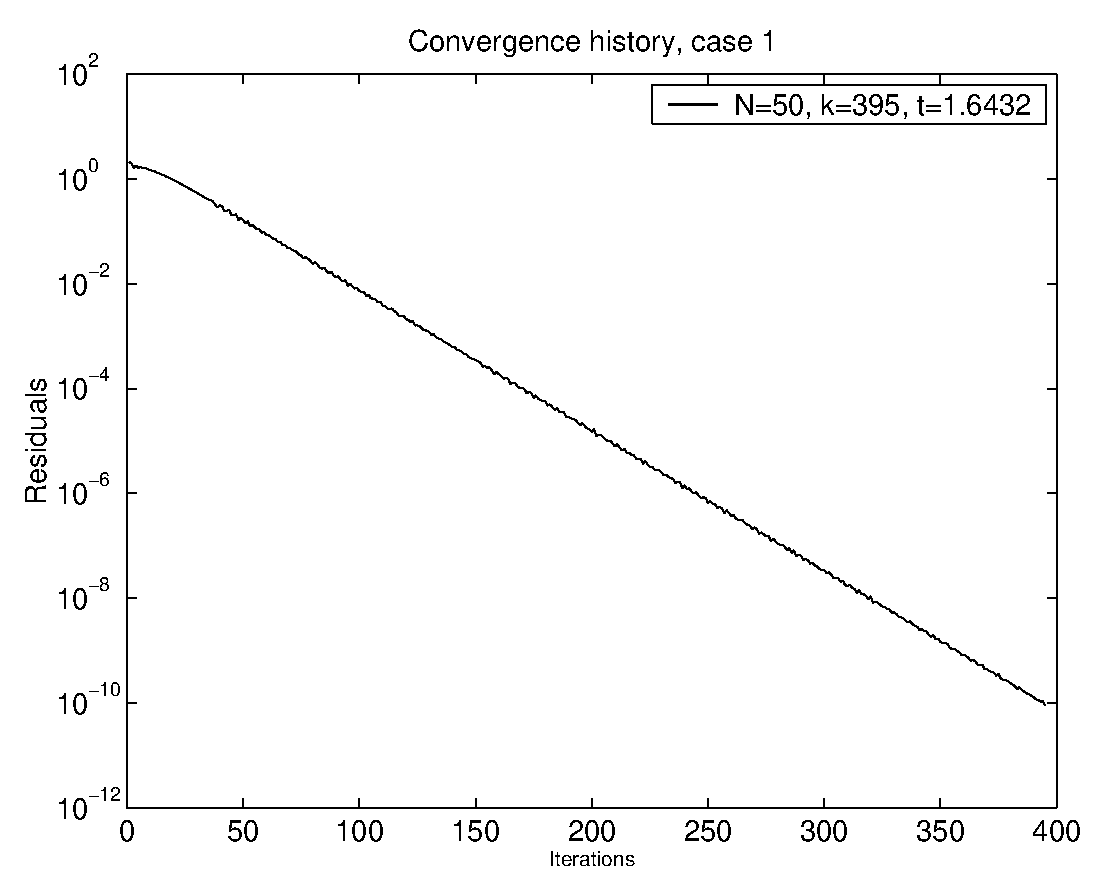
\includegraphics[scale=0.35]{eps/tscheb1.eps}\hfill\includegraphics[scale=0.35]{eps/tscheb2.eps} \\
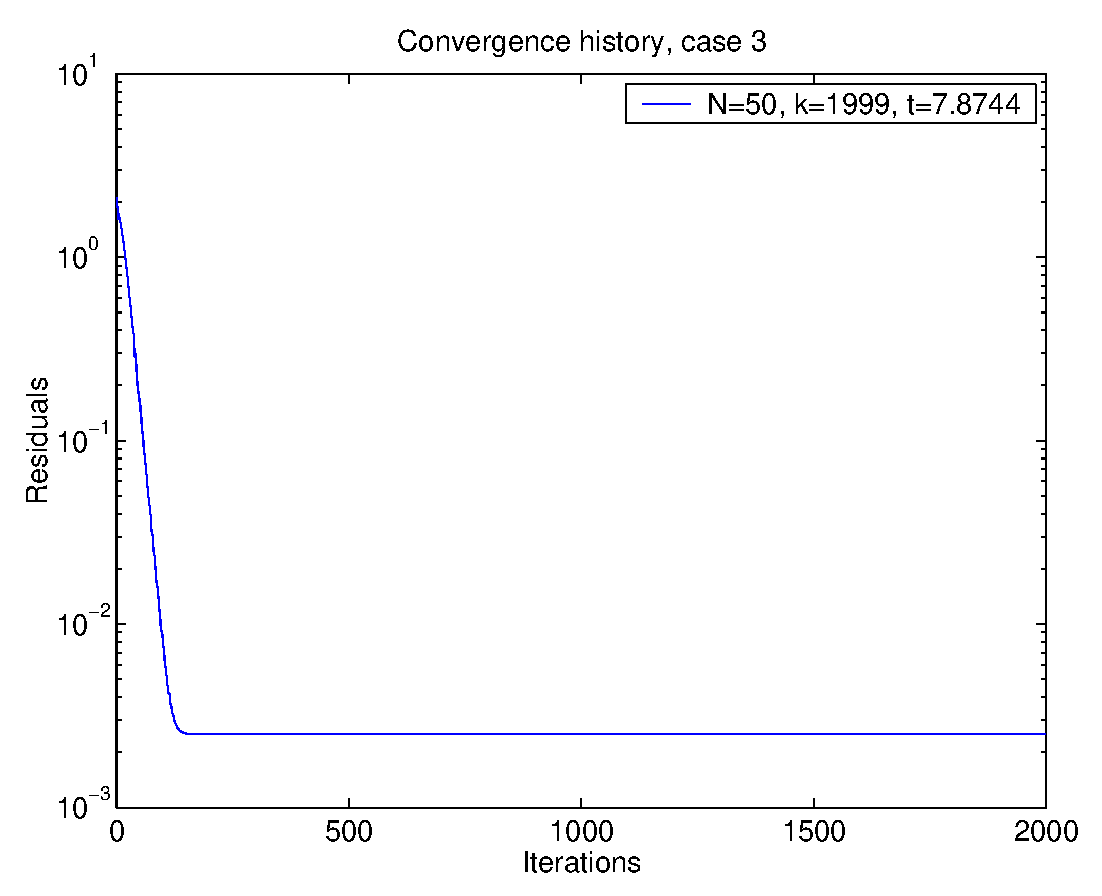
\includegraphics[scale=0.35]{eps/tscheb3.eps}\hfill\includegraphics[scale=0.35]{eps/tscheb4.eps} \\
\includegraphics[scale=0.35]{eps/tscheb5.eps}\hfill {}
\caption{Numerische Resultate f"ur das Modellproblem auf einem $50 \times 50$-Gitter}
\end{figure}

\section[Analyse von Tschebyscheff- und...]{Analyse von Tschebyscheff- und Ri\-chard\-son-Ver\-fahren}

\begin{sa} \label{Tscheb_analyse_sa}
  Sei $p_m$ das Polynom des Tschebyscheff-Verfahrens
  bzgl.\ $E(f_1,f_2,\rho)\not\ni 0$ mit $\spek(A)\subseteq E(f_1,f_2,\rho)$.
  Dann gilt
  \begin{equation*}
    r^m=p_m(A)r^0
  \end{equation*}
  und damit f�r jede Norm $\norm{\cdot}$
  \begin{equation*}
    \norm{r^m}\leq\norm{p_m(A)}\cdot\norm{r^0}.
  \end{equation*}
  \begin{enumerate}
  \item
    \label{TschVerf-analyse-satz1}
    Es sei $A$ diagonalisierbar mit $A=SDS^{-1}$ (siehe \ref{Konvergenzdiag_kor})
    und $\norm{}$ sei die Norm $\norm{}_S$.
    Dann gilt
    \begin{equation*}
      \norm{p_m(A)}
      \leq
      \frac{\rho^m+\rho^{-m}}{\,\abs{w_\gamma^m+w_\gamma^{-m}}\,},
    \end{equation*}
    wobei $w_\gamma$ (betragsgr��te)
    L�sung von $\frac{1}{2}(w+w^{-1})=-b/a$.
  \item Ist in \ref{TschVerf-analyse-satz1}. sogar $S$ orthogonal
    (z.B. weil $A$ normal ist), so gilt sogar
    \begin{equation*}
      \norm{p_m(A)}_2
      \leq
      \frac{\rho^m+\rho^{-m}}{\,\abs{w_\gamma^m+w_\gamma^{-m}}\,}.
    \end{equation*}
  \end{enumerate}
\end{sa}

\begin{proof}
  Ist $q_m$ die approximative Optimall�sung f"ur die Ellipse $E(-1,1,\rho)$ mit
  $q_m(\gamma) = 1$, dann gilt nach Satz~\ref{cmschranke_sa}
  \begin{equation*}
    \max_{t\in E(-1,1,\bar{\rho})}\abs{q_m(t)}
    =
    \frac{\bar{\rho}^m+\bar{\rho}^{-m}}{\,\abs{w_\gamma^m+w_\gamma^{-m}}\,}.
  \end{equation*}
  Mit der affinen Transformation $z\mapsto az+b$ aus Lemma~\ref{ellipsentransf_lem},
  welche $E(-1,1,\rho)$ auf
  $E(f_1,f_2,\rho)$ abbildet, ergibt sich der Satz.
\end{proof}
\medskip

Besonders wichtig ist der Fall $\spek(A)\subseteq[\xi,\Xi]\subseteq(0,+\infty)$
und $A$ symmetrisch und positiv definit:

\begin{cor} \label{Tscheb_pos_def_cor}
  Ist $\spek(A)\subseteq[\xi,\Xi]\subseteq(0,+\infty)$
  und $A$ spd, dann gilt f�r die Residuen des Tschebyscheff-Verfahrens
  \begin{equation*}
    \norm{r^m}_2\leq\norm{p_m(A)}_2\cdot\norm{r^0}_2
  \end{equation*}
  mit
  \begin{equation*}
    \norm{p_m(A)}_2
    \leq
     \frac{2c^m}{1+c^{2m}} \enspace
     \mbox{ mit } c = \frac{\sqrt{\kappa}-1}{\sqrt{\kappa}+1}, \,
    \kappa = \frac{\Xi}{\xi}.
  \end{equation*}
\end{cor}

\begin{proof}
  Hier ist $f_1=\xi$, $f_2=\Xi$, $\rho = 1$, $a= \frac{1}{2}(\Xi - \xi), b = \frac{1}{2}(\Xi+\xi)$ und $\gamma = -b/a$. Aus
Satz~\ref{Tscheb_analyse_sa} folgt so
\[
   \norm{p_m(A)}_2 \leq \frac{2}{\,\abs{w_\gamma^m+w_\gamma^{-m}}\,} 
\]
mit
\begin{equation*}
\frac{1}{2}(w_\gamma+w_\gamma^{-1})=-\frac{b}{a}=- \frac{\Xi+\xi}{\Xi-\xi}=
    -\frac{\kappa+1}{\kappa-1}.
\end{equation*}
Auf\/l�sen der quadratischen Gleichung ergibt
\begin{eqnarray*}
  w_\gamma &=& - \frac{\kappa+1}{\kappa-1} -          \sqrt{\left(\frac{\kappa+1}{\kappa-1}\right)^2-1} \\
   &=& - \frac{\kappa+1}{\kappa-1} - \sqrt{\frac{4\kappa}{(\kappa-1)^2}} \\
   &=& - \frac{\kappa+1}{\kappa-1} - \frac{2\sqrt{\kappa}}{\kappa-1} \\
   &=& - \frac{\left(\sqrt{\kappa}+1\right)^2}{(\sqrt{\kappa}-1)(\sqrt{\kappa}+1)} \\
   &=& -\frac{\sqrt{\kappa}+1}{\sqrt{\kappa}-1}.
\end{eqnarray*}

\end{proof}


Zum Abschluss (und Vergleich) analysieren wir noch das Richardson-Ver\-fahr\-en
2.~Ordnung. Dazu sei $A$ spd mit $\spek(A)\subseteq[\xi,\Xi]$.

\begin{aufg}
  F�r das relaxierte Richardson-Verfahren 1.~Ordnung
  \begin{equation*}
    x^{m+1} = x^m+\alpha r^m
  \end{equation*}
  wird f�r die zugeh�rigen Polynome $p_m(z)=(1-\alpha z)^m$ die Gr��e
  \begin{equation*}
    \max_{z\in[\xi,\Xi]}\abs{p_m(z)}
  \end{equation*}
  minimal, wenn $\alpha=2/(\xi+\Xi)$.
\end{aufg}

\begin{bem}
  Das relaxierte Richardson Verfahren 1.~Ordnung $Ax=b$ ist �quivalent zum
  gew�hnlichen Richardson-Verfahren 1.~Ordnung f"ur
  \begin{equation*}
    (\alpha A)x = \alpha b,
  \end{equation*}
  also
  \begin{equation*}
    x^{m+1} = x^m+(\alpha b-\alpha A x^m).
  \end{equation*}
  Wir gehen ab jetzt davon aus, dass diese "`Skalierung"' des
  LGS (mit $\alpha=\frac{2}{\xi+\Xi})$ bereits erfolgte, d.h.\ es gilt ab jetzt
  \begin{equation*}
    \spek(A) \subseteq [1-\gamma, 1+\gamma]
    \text{ mit }
    \gamma = \frac{\Xi-\xi}{\Xi+\xi} \in [0,1).
  \end{equation*}
\end{bem}

F�r das System
\begin{equation*}
  Ax=b
\end{equation*}
betrachten wir jetzt das Richardson-Verfahren 2.~Ordnung

%%$$\norm{p_m(A)}_{s/2}\leq \max_{\lambda\in
%%E(f_1,f_2,\rho)}\abs{p_m(\lambda)}
%%=\frac{\rho^m+\pfrac{1}{s}^m}{\abs{w_\gamma^m+\pfrac{1}{w_\gamma}^m}}$$
%%
%%\begin{equation*}
%%  \frac{1}{2}(w_\gamma+w_\gamma^{-1})=-\frac{b}{a}
%%  \text{ mit }
%%  \abs{w_\gamma} >\rho.
%%\end{equation*}
%%Diskussion der oberen Schranke:
%%
%%-----------------------------
%%
%%BILD 1
%%
%%Experimente mit falschem Intervall liefern: Es kann immer noch
%%konvergieren. Die Konvergenz ist aber am schnellsten, wenn das
%%richtige Intervall gew�hlt wird.
%%
%%
%%
%%\textbf{Richardson 1.~Ordnung}
%%
%%$$Ax=b$$
%%
%%$$(\alpha A)x=\alpha b$$
%%
%%$$\spek(A)\subseteq[1-\gamma,1+\gamma]$$
%%$$x=(I-A)x+b$$
%%%%$$x=Bx+b,\qquad \spek(B)\subseteq[-\gamma,+\gamma]$$

\begin{align*}
  x^{m+1}
  &=
  \omega\bigl((I-A)x^m+b\bigr)+(1-\omega)x^{m-1}\\
  &=
  \omega(x^m+r^m)+(1-\omega)x^{m-1}
\end{align*}
mit
\begin{align*}
  r^{m+1} &= \omega r^m-\omega Ar^m+(1-\omega)r^{m-1}, \\
  p_{m+1} &= \omega(1-t)p_m(t)+(1-\omega)p_{m-1}(t).
\end{align*}
Daraus folgt

\begin{equation*}
  \begin{pmatrix}
    p_{m+1}(t) \\ p_m(t)
  \end{pmatrix}
  =
  \underbrace{
    \begin{pmatrix}
      \omega(1-t) & 1-\omega\\
      1 & 0
    \end{pmatrix}
  }_{B_\omega(t)}
  \begin{pmatrix}
    p_{m}(t) \\ p_{m-1}(t)
  \end{pmatrix} .
\end{equation*}
Wir wollen nun das \glqq{}optimale\grqq{} $\omega$ ermitteln,
d.h.\ wir suchen die L�sung  $\omega$ von
\begin{equation}
  \label{Richardsonmin_eq}
  \min_{\omega\in\rr\mathstrut}\,
  \max_{t\in[1-\gamma,1+\gamma]}
  \rho\bigl(B_\omega(t)\bigr).
\end{equation}

Zur besseren Darstellung machen wir den �bergang $t \to 1-t$, also
\begin{eqnarray*}
  1-t &\lr& t \in [-\gamma,\gamma],
  \\
  B_\omega(t)
  &=&
  \begin{pmatrix}
    \omega(1-t) & 1-\omega\\
    1 & 0
  \end{pmatrix}
  \lr
  \begin{pmatrix}
    \omega t & 1-\omega\\
    1 & 0
  \end{pmatrix}.
\end{eqnarray*}
Wir suchen damit die L�sung $\omega$ der Minimierungsaufgabe
\begin{equation*}
  \min_{\omega\in\rr\mathstrut}\,
  \max_{t\in[-\gamma,\gamma]}
    \rho\bigl(B_\omega(t)\bigr).
\end{equation*}

Nun bestimmen wir die Eigenwerte $\lambda$ von $B_\omega(t)$. Es gilt n�mlich
\begin{align*}
  (\lambda-\omega t)\lambda-(1-\omega) &= 0 \\
  \iff
  \lambda^2-(\omega t)\lambda-(1-\omega) &= 0,
\end{align*}
d.h.\ wir erhalten
\begin{align*}
  \lambda_{1,2}
  &=
  \frac{\omega t}{2}
  \pm
  \sqrt{
    \frac {\omega^2t^2} {4} + (1-\omega)
  }
  \,.
\end{align*}

Wir machen zun�chst eine
Fallunterscheidung zur Berechnung von $\rho\bigl(B_\omega(t)\bigr)$.

\textit{Fall I}: $\dfrac{\omega^2t^2}{4}+(1-\omega) < 0$.
Dann gilt
\begin{align*}
  \abs{\lambda_{1,2}}^2
  &=
  \frac{(\omega t)^2}{4}+\frac{(\omega t)^2}{4}+(1-\omega) \\
  &=
  \frac{(\omega t)^2}{2}+(1-\omega). \\
\end{align*}
Also gilt
\begin{equation}
  \label{Richardson:FallI_eq}
  \rho\bigl(B_\omega(t)\bigr)
  =
  \biggl(
  \frac {(\omega t)^2} {2} + (1-\omega)
  \biggr)^{\!\! 1/2}.
\end{equation}

\textit{Fall II}: $\dfrac{\omega^2t^2}{4}+(1-\omega)\geq0$.

(a) $\omega t\geq 0$: In diesem Fall haben wir
\begin{equation*}
  \rho\bigl(B_\omega(t)\bigr)
  =
  \frac{\omega t}{2}+\sqrt{\frac{\omega^2t^2}{4}+(1-\omega)}.
\end{equation*}

(b) $\omega t\leq 0$: Dann gilt
\begin{equation*}
  \rho\bigl(B_\omega(t)\bigr)
  =
  \abs{\frac{\omega t}{2}-\sqrt{\frac{\omega^2t^2}{4}+(1-\omega)}}.
\end{equation*}

In beiden F�llen (a) und (b) erhalten wir aber
\begin{equation}
  \label{Richardson:FallII_eq}
  \rho\bigl(B_\omega(t)\bigr)
  =
  \frac {\abs{\omega t}} {2} + \sqrt{\frac{\omega^2t^2}{4}+(1-\omega)}.
\end{equation}


Sei nun $\omega$ fest. Wir bestimmen
$\max\limits_{t\in[-\gamma,\gamma]}\rho\bigl(B_\omega(t)\bigr)=:\beta_\omega$.

\textit{1.~Fall}: $\omega \leq 1$. Es kommt nur Fall~II vor.  Aus
\eqref{Richardson:FallII_eq} erhalten wir, da $\rho\left(B_\omega(t)\right)$ eine
gerade Funktion ist und monoton wachsend f�r $t\in[0,\gamma]$
\begin{equation*}
  \beta_\omega
  =
  \frac {\abs{\omega}\gamma} {2}
  + \sqrt { \frac {\omega^2\gamma^2} {4} + (1-\omega) }.
\end{equation*}

\textit{2.~Fall}: $\omega>1$. Jetzt kommen Fall~I und Fall~II beide vor.
Es gilt
\begin{equation*}
  \frac {\omega^2t^2} {4} + (1-\omega)
  \geq 0
  \iff
  \abs{t} \geq \frac {2\sqrt{\omega-1}} {\omega}.
\end{equation*}
Dann ist
\begin{equation*}
  \rho\bigl(B_\omega(t)\bigr)
  =
  \frac {\omega \abs{t}} {2}
  + \sqrt { \frac {\omega^2t^2} {4} + (1-\omega) }.
\end{equation*}

Im Fall $\abs{t}\leq \dfrac{2\sqrt{\omega-1}}{\omega}$ ist
\begin{equation*}
  \rho\bigl(B_\omega(t)\bigr)
  =
  \left(
    \frac {(\omega t)^2} {2} + (1-\omega)
  \right)^{\!\!\! 1/2}\negthickspace,
\end{equation*}
also ist
\begin{multline*}
  \beta_\omega
  =
  \max
  \Biggl\{
    \max_{\abs{t}\leq\frac{2\sqrt{\omega-1}}{\omega}}
    \left(
      \frac {(\omega t)^2} {2} + (1-\omega)
    \right)^{\!\!\! 1/2}
    \negthickspace,
    \\
    \max_{\frac{2\sqrt{\omega-1}}{\omega}\leq\abs{t}\leq\gamma}
    \left(
      \frac {\omega\abs{t}} {2}
      + \sqrt { \frac {(\omega t)^2} {4} + (1-\omega) \! } \:
    \right)
  \Biggr\}.
\end{multline*}

Hierin kommt der erste Term nur vor, wenn $\gamma\geq
\frac{2\sqrt{\omega-1}}{\omega}$. Aus Monotoniegr�nden folgt
\begin{align*}
  \max_{\abs{t}\leq\frac{2\sqrt{\omega-1}}{\omega}}
  \left(\frac{(\omega t)^2}{2}+(1-\omega)\right)^{\!\!\! 1/2}
  &=
  \left(
    \frac {\bigl( \omega \frac {2\sqrt{\omega-1}} {\omega} \bigr)^2} {2}
    + (1-\omega)
  \right)^{\!\!\! 1/2}
  \\
  &=
  \sqrt{\omega-1}
  ,
  \\
  \max_{\frac{2\sqrt{\omega-1}}{\omega}\leq\abs{t}\leq\gamma}
  \left(
    \frac {\omega\abs{t}} {2}
    + \sqrt { \frac {(\omega t)^2} {4} + (1-\omega) \! } \:
  \right)
  &=
  \frac{\omega\gamma}{2}
  + \sqrt{ \frac {(\omega\gamma)^2} {4} + (1-\omega) }
  .
\end{align*}
F�r $\gamma\geq\frac{2\sqrt{\omega-1}}{\omega}$ gilt
\begin{align*}
  \frac{\omega\gamma}{2}
  + \sqrt{ \frac {(\omega\gamma)^2} {4} + (1-\omega) }
  &\geq
  \frac {\,\omega\frac{2\sqrt{\omega-1}}{\omega}\,} {2}
  +
  \sqrt {
    \frac {\bigl(\omega\frac{2\sqrt{\omega-1}}{\omega}\bigr)^2} {4}
    + (1-\omega)
  }
  \\
  &=
  \sqrt{\omega-1}
  .
\end{align*}
Damit gilt
\begin{equation*}
  \beta_\omega
  =
  \begin{cases}
    \sqrt{\omega-1}
    & \text{falls }
    \gamma<\frac{2\sqrt{\omega-1}}{\omega},
    \\
    \dfrac{\omega\gamma}{2}+\sqrt{\dfrac{(\omega\gamma)^2}4{}+(1-\omega)}
    & \text{falls }
    \gamma \geq \frac{2\sqrt{\omega-1}}{\omega}.
  \end{cases}
\end{equation*}
Unter Beachtung von
\begin{align*}
  &\gamma < \frac{2\sqrt{\omega-1}}{\omega} \\
  \iff&
  \omega^2\gamma^2 < 4(\omega-1) \\
  \iff&
  \frac{2-2\sqrt{1-\gamma^2}}{\gamma^2}
  < \omega <
  \frac{2+2\sqrt{1-\gamma^2}}{\gamma^2} \\
  \iff&
  \frac{2}{1+\sqrt{1-\gamma^2}}
  < \omega <
  \frac{2}{1-\sqrt{1-\gamma^2}}
\end{align*}
erhalten wir durch Zusammenfassen von "`1.~Fall"' und "`2.~Fall"'

\begin{equation*}
  \beta_\omega
  =
  \begin{cases}
    \sqrt{\omega-1}
    & \text{falls }
    \frac {2} {1+\sqrt{1-\gamma^2}} < \omega < \frac {2} {1-\sqrt{1-\gamma^2}}
    ,
    \\
    \frac{\omega\gamma}{2}+\sqrt{\frac{(\omega \gamma)^2}{4}+(1-\omega)}
    & \text{sonst.}
  \end{cases}
\end{equation*}

F�r $\omega\geq 2/\bigl(1-\sqrt{1-\gamma^2\!}\:\bigr)\;(\geq2)$
ist $\frac{\omega\gamma}{2}\geq \sqrt{\omega-1}\geq 1$, also
$\beta_\omega\geq 1$.
F�r $\omega < 2/\bigl(1+\sqrt{1-\gamma^2\!}\:\bigr)$ ist
\begin{equation*}
  \beta_\omega
  =
  \frac{\omega\gamma}{2}
  + \sqrt{\frac{(\omega\gamma)^2}{4}+(1-\omega)}
\end{equation*}
monoton fallend. Die Gr��e $\beta_\omega$ wird also minimal f�r
$\omega=\omega_0=\frac{2}{1+\sqrt{1-\gamma^2}}$ und hat dann den Wert
$\sqrt{\omega_0-1}$.

Zusammenfassend erhalten wir also:
\begin{sa}
  Der optimale Parameter $\omega$ f�r das Richardson-Verfahren
  2.~Ordnung, welcher die Minimierungsaufgabe \eqref{Richardsonmin_eq}
  l�st, ist
  \begin{equation*}
    \omega_0
    =
    \frac {2} {1+ \sqrt{1-\gamma^2}}
    \,.
  \end{equation*}
\end{sa}

Jetzt kann man f\"ur $ w = w_0 $ die Gr\"o\ss{}e

\[
\underset{t \in \left[ 1-\gamma , 1 + \gamma \right] }{\max} \left| p_m(t) \right|
\]

diskutieren unter Beachtung von $p_0 = 1$, $p_1(t) = 1-t$.

\begin{aufg} Bestimme f\"ur alle $t \in \left[ 1 - \gamma, 1 + \gamma \right] $ die L\"osung der
Differenzengleichung 2.~Ordnung
\[
p_{m+1}(t) = w_0 \cdot (1-t) p_m(t) + (1-w_0) p_{m-1}(t)
\]
unter den Anfangsbedingungen $ p_0 = 0$ und $ p_1(t) = 1-t $ und zeige damit
\begin{enumerate}
\item
$
\underset{t \in \left[ 1-\gamma , 1 + \gamma \right] }{\max} \left| p_m(t) \right| =
\left( \sqrt{w_0 - 1} \right)^m (1+m\sqrt{1-\gamma^2}) =: \rho_m,
$
(Dies ist sehr aufwendig!\footnote{Man liest also besser bei den Meistern nach:
G. Golub, R. Varga: Chebyshev semi-iterative methods, successive overrelaxation iterative
methods and second-order Richardson iterative methods, Part I and II, Numer. Math. {\bf 3},
 147-168 (1961).})
\item $ \rho_m $ f\"allt monoton in $m$,
\item $ \rho_m > c_m $,  $c_m = \frac{2c^{m}}{1+c^{2m}}$
aus dem Tschebyscheff Verfahren mit $c = \frac{\sqrt{\kappa} - 1}{\sqrt{\kappa}+1}$, $\kappa = \frac{1+\gamma}{1-\gamma} $,
\item es gilt $ \limn \frac{\rho_m}{c_m} = 1 $.
\end{enumerate}
\end{aufg}

\begin{bem}
Aus $ r^m = p_m(A) r^0$ folgt $e^m =  p_m(A) e^0$ mit $e^m = A^{-1}b - x^m$ und damit
\[
\|e^m\| \leq \| p_m(A) \| \|e^0\|.
\]
\end{bem}
Tschebyscheff- und Richardson-Verfahren machen eine Schranke
f"ur $\|p_m(A)\|$ klein. Dies wirkt sich demnach in den  Absch"atzungen
nicht nur f\"ur das Residuum, sondern auch
f"ur den {\em Fehler} aus.

%%% Local Variables:
%%% mode: latex
%%% TeX-master: "Iterationsverfahren03"
%%% End:

\section{Basen f\"ur Krylov-Unterr\"aume}

Gegeben: $A \in \cnn$ nicht notwendigerweise hermitesch, $A$ regul�r,
\[
K_m = \langle r, Ar,...,A^{m-1}r \rangle.
\]

Gesucht: $v^1,...,v^m$ mit "`sch\"onen Eigenschaften"' und
\[
K_m = \langle v^1,...,v^m \rangle.
\]

{\bf Erinnerung:} Gram-Schmidt-Orthogonalisierung

Gegeben: $y_1,...,y_m \in \cnn$.

\begin{alg}[Gram-Schmidt-Orthogonalisierung, klassisch] \label{Gram-Schmidt-Verfahren instabil}
~\vspace*{-2\baselineskip}
\begin{algorithm}
  \begin{algorithmic}
    \STATE $v^i = y^i, \; i=1,\ldots,m$
    \FOR{$i = 1, \dots,m$}
      \FOR{$j = 1, \dots ,i-1$}
        \STATE $v^i = v^i - \langle y^i,v^j\rangle v^j$
      \ENDFOR
      \STATE $v^i = \frac{1}{\|v^i\|} \cdot v^i$
    \ENDFOR
  \end{algorithmic}
\end{algorithm}
\end{alg}

Es ist bekannt, dass diese Variante aber numerisch nicht stabil ist.
G"unstiger ist es, wenn man bei der Berechnung der Innenprodukte statt $y_i$
den aktuellen Vektor $v^i$ verwendet. Dies ist m"oglich, da zu jedem
Zeitpunkt der $j$-Schleife der Vektor $y^i-v^i \in \langle v^1,
\ldots,v^{j-1} \rangle$  senkrecht auf $v^j$ steht.

\begin{alg}[modifizierte Gram-Schmidt-Orthogonalisierung] \label{modifizieres Gram-Schmidt-Verfahren}
~                               % um "x.x Algorithmus" aus dem Kasten rauszubekommen
\vspace*{-2\baselineskip}       % um den Leeraum zu entfernen
\begin{algorithm}
  %\caption{modifiziertes Gram-Schmidt-Verfahren. }
  \begin{algorithmic}
    \STATE $v^i = y^i\; i=1,\ldots,m$
    \FOR{$i = 1, \dots,m$}
      \FOR{$j = 1, \dots ,i-1$}
        \STATE $v^i = v^i - \langle v^i,v^j\rangle v^j$
      \ENDFOR
      \STATE $v^i = \frac{1}{\|v^i\|} \cdot v^i$
    \ENDFOR
  \end{algorithmic}
\end{algorithm}
\end{alg}

Unser Ziel ist es, sukzessive eine ONB von $K_m(A,r)$ aufzubauen.

\medskip

{\bf Idee:}

$\langle v^1,...,v^m\rangle$ sei eine ONB in $K_m(A,r)$ mit $v^m \notin K_{m-1}(A,r)$. Dann
gilt insbesondere $A v^m \in K_{m+1}(A,r)\setminus K_m(A,r)$. Orthogonalisiere also $Av^m$ gegen $v^1,...,v^m$.

Durch Anwendung des modifizierten Gram-Schmidt-Verfahrens resultiert
das {\em Arnoldi-Verfahren}.

\begin{alg}[Arnoldi-Verfahren] \label{Arnoldi-Verfahren}
~  				% um "3.3 Algorithmus" aus dem Kasten rauszubekommen
\vspace*{-2\baselineskip}	% um den Leeraum zu entfernen
\begin{algorithm}
  %\caption{Arnoldi-Verfahren}
  \begin{algorithmic}
    \STATE $v^1 = r$, $h_{1,0} = \|r\|$, $v^1 = \frac{1}{h_{1,0}}r$
    \FOR{$i = 2, 3, \dots$}
      \STATE $v^i = Av^{i-1}$
      \FOR{$j = 1, \dots ,i-1$}
        \STATE $h_{j,i-1} = \langle v^i,v^j\rangle$
        \STATE $v^i = v^i - h_{j,i-1} v^j$
      \ENDFOR
      \STATE $h_{i,i-1} = \| v^i \|$
      \STATE $v^i = \frac{1}{h_{i,i-1}} \cdot v^i$
    \ENDFOR
  \end{algorithmic}
\end{algorithm}
\end{alg}

Wir f\"uhren folgende Kurznotation ein

\begin{equation}
\label{obereHessenbergmatrix} A V_m = V_{m+1} H_{m+1,m}
\end{equation}

mit

\[
V_m = \left[ v^1,...,v^m \right] \in \co^{n \times m}
\]

\[
H_{m+1,m}=\left(\begin{array}{cccc}
h_{1,1} & h_{1,2}& \cdots & h_{1,m}\\
h_{2,1} & h_{2,2} &\ddots & h_{2,m}\\
&\ddots&\ddots&\vdots \\
&&\ddots& h_{m,m}\\
&&& h_{m+1,m}
\end{array}\right) \in \co^{(m+1)\times m}.
\]

Im Falle $ A = A^H $ vereinfacht sich der Arnoldi-Prozess, da
die meisten Eintr"age in $H_{m+1,m}$ verschwinden. Es bezeichne
dazu $H_m$ die Matrix
\[
H_m = \left(\begin{array}{cccc}
h_{1,1} & h_{1,2}& \cdots & h_{1,m}\\
h_{2,1} & h_{2,2} &\ddots & h_{2,m}\\
&\ddots&\ddots&\vdots \\
&& h_{m-1,m} & h_{m,m}
\end{array}\right) \in \co^{m\times m}.
\]

\begin{lem}
Falls $A$ hermitesch ist, ist  $H_m$ eine reelle, symmetrische Tridiagonalmatrix.
Es gilt also $h_{i+1,i} = h_{i,i+1}$ f"ur alle $i$ und $h_{i,j} = 0 $ f"ur $i > j+1$.
\end{lem}

\begin{proof}
Aus \eqnref{obereHessenbergmatrix} folgt

\begin{align*}
V_m^H A V_m &= V_m^H V_{m+1} H_{m+1,m} \\
            &= \left(\begin{array}{cc}
                        & 0\\
                        & \vdots\\
\quad                        \raisebox{12pt}[-12pt]{\Large $I_m$} \quad& 0 \\
               \end{array}\right) H_{m+1,m} \\
            &= H_m.
\end{align*}
Mit $V_m^HAV_m$ ist auch $H_m$ hermitesch, besitzt also Tridiagonalgestalt.
Au"serdem sind dann die Diagonalelemente reell (und positiv). Die Elemente
$h_{i,i-1}$ der ersten Nebendiagonalen ergeben sich nach
Algorithmus~\ref{Arnoldi-Verfahren}  als $\|v^i\|$, sind also auch reell.
\end{proof}

Damit erhalten wir aus dem Arnoldi-Verfahren das Lanczos-Verfahren zur Bestimmung einer ONB von
$K_m(A,r)$ im Falle $A = A^H$.

\begin{alg}[Lanczos-Verfahren] \label{Lanczos-Verfahren0}
~  				% um "3.3 Algorithmus" aus dem Kasten rauszubekommen
\vspace*{-2\baselineskip}	% um den Leeraum zu entfernen
\begin{algorithm}
  %\caption{Lanczos-Verfahren}
  \begin{algorithmic}
    \STATE $v^1 = \frac{r}{\|r\|}, \; v^0 = 0,\; h_{1,0} = 0$
    \FOR{$i = 2,3, \dots$}
      \STATE $v^i = Av^{i-1}$
      \STATE $v^i = v^i - h_{i-1,i-2}v^{i-2}$
      \STATE $h_{i-1,i-1} = \langle v^i,v^{i-1}\rangle$
      \STATE $v^i = v^i - h_{i-1,i-1}v^{i-1}$
      \STATE $h_{i,i-1} = \|v_i\|$
      \STATE $v^i = \frac{1}{h_{i,i-1}}\cdot v^i$
    \ENDFOR
  \end{algorithmic}
\end{algorithm}
\end{alg}

Eine alternative Bezeichnung f"ur die Koeffizienten im Lanczos-Verfahren ist

\[
h_{i-1,i-2} = \beta_{i-1}, \enspace
h_{i-1,i-1} = \alpha_{i-1}.
\]

Damit l�sst sich der Algorithmus wie folgt formulieren:

\begin{alg}[Lanczos-Verfahren] \label{Lanczos-Verfahren}
~               % um "3.3 Algorithmus" aus dem Kasten rauszubekommen
\vspace*{-2\baselineskip}   % um den Leeraum zu entfernen
\begin{algorithm}
  %\caption{Lanczos-Verfahren}
  \begin{algorithmic}
    \STATE $v^1 = \frac{r}{\|r\|}, \; v^0 = 0,\; \beta_1 = 0$
    \FOR{$i = 2,3, \dots$}
      \STATE $q^i = Av^{i-1} - \beta_{i-1} v^{i-2}$
      \STATE $\alpha_{i-1} = \langle q^i,v^{i-1} \rangle$
      \STATE $q^i = q^i - \alpha_{i-1} v^{i-1}$
      \STATE $\beta_{i} = \|q^i\|$
      \STATE $v^i = \frac{q^i}{\beta_{i}}$
    \ENDFOR
  \end{algorithmic}
\end{algorithm}
\end{alg}

Hierin gilt:
\begin{equation}
\label{betamalalpha} \beta_{i} v^i = A v^{i-1} - \alpha_{i-1} v^{i-1} - \beta_{i-1} v^{i-2}.
\end{equation}

\begin{defn}
Zwei Folgen $v^1,\cdots ,v^m$ und $w^1,\cdots ,w^m \in \cn $ hei�en {\em bi-orthogonal},
falls gilt
\[
\langle v^i,w^j \rangle  = \delta_{i,j}.
\]
\end{defn}

\begin{bem}
$v^i,w^j$ sind nur bis auf reziproke Vielfache eindeutig bestimmt.
\end{bem}

Im Falle $A \neq A^H$ konstruieren wir nun eine bi-orthogonale Basis $v^1,\cdots ,v^m$ von $K_m(A,r)$ und
$w^1,\cdots ,w^m$ von $K_m(A^H,\tilde{r})$.

\bigskip

Man berechnet $v^1,w^1$ mit dem {\em unsymmetrischen} Lanczos-Verfahren.

\bigskip

{\bf Situation:}
\begin{quote}
$v^1,\ldots, v^m$ sei eine Basis von $K_m(A,r)$

$w^1,\ldots, w^m$ sei eine Basis von $K_m(A^H,\tilde{r})$

die beiden Basen sind bi-orthogonal
\end{quote}
und
\begin{quote}
$v^m \notin K_{m-1}(A,r)$

$w^m \notin K_{m-1}(A^H,\tilde{r})$.
\end{quote}

{\bf Ansatz:}
\begin{align*}
q^{m+1} &= Av^m,\\
p^{m+1} &= A^Hw^m.
\end{align*}
Wir setzen an:
\begin{align}
\tilde{v}^{m+1} &= q^{m+1} - \sum_{i=1}^m \alpha_i v^i,\\
\tilde{w}^{m+1} &= p^{m+1} - \sum_{i=1}^m \beta_i w^i.
\end{align}

{\bf Bedingung f"ur Bi-Orthogonalit"at:}
\begin{align*}
\langle \tilde v^{m+1},w^j \rangle =& \langle q^{m+1},w^j \rangle -\alpha_j \overset{!}{=} 0,\\
\langle v^{j}, \tilde w^{m+1} \rangle =& \langle v^j,p^{m+1} \rangle -\overline{\beta}_j \overset{!}{=} 0.
\end{align*}

Damit erhalten wir
\begin{align*}
\alpha_j =&\langle q^{m+1},w^j \rangle,\\
\beta_j =&\langle p^{m+1},v^j \rangle.
\end{align*}

F�r $ j \leq m-2$ gilt allerdings weiter
\begin{align*}
\alpha_j =\langle q^{m+1},w^j \rangle
                       &=\langle Av^m,w^j \rangle \\
                       &=\langle v^m,A^Hw^j \rangle \\
                       &=0,
\end{align*}
da $A^Hw^j \in K_{m-1}(A^H,\tilde{r})$. Analoges gilt f"ur die $\beta_j$, d.h.\ es
 gilt
\[
\alpha_j = \beta_j = 0 \mbox{ f"ur } j=1,\ldots,m-2.
\]

Zur Normierung sei
\begin{align*}
\delta_{m+1} &= \left( \langle \tilde{v}^{m+1},\tilde{w}^{m+1} \rangle \right) ^{\frac 12}\\
v^{m+1} &= \frac{1}{\delta_{m+1}}\tilde{v}^{m+1} \\
w^{m+1} &= \frac{1}{\overline{\delta}_{m+1}}\tilde{w}^{m+1}
\end{align*}
Schlie"slich weisen wir noch nach, dass die Koeffizienten $\alpha_{m-1}$ und
$\beta_{m-1}$ vom vorherigen Schritt schon bekannt sind (daf"ur verwenden wir
kurzfristig einen zus"atzlichen oberen Index):
\begin{align*}
\alpha_{m-1} &= \langle Av^m,w^{m-1}\rangle\\
 &= \langle v^m,A^Hw^{m-1} \rangle\\
 &= \langle v^m,\tilde{w}^m + \beta_{m-1}^{(m-1)} w^{m-1} + \beta_{m-2}^{(m-1)} w^{m-2} \rangle\\
 &= \langle v^m,\tilde{w}^m \rangle = \delta_{m}
\intertext{ }
\beta_{m-1} &= \langle A^Hw^m,v^{m-1} \rangle\\
 &= \langle w^m,Av^{m-1} \rangle \\
 &= ...\\
 &= \langle w^m,\tilde{v}^m\rangle = \overline{\delta}_{m}
\end{align*}

Insgesamt erhalten wir damit folgendes Verfahren:

\begin{alg}[unsymmetrisches Lanczos-Verfahren] \label{unsymmetrisches Lanczos-Verfahren}
~               % um "3.3 Algorithmus" aus dem Kasten rauszubekommen
\vspace*{-2\baselineskip}   % um den Leeraum zu entfernen
\begin{algorithm}
  %\caption{Lanczos-Verfahren}
  \begin{algorithmic}
    \STATE $v^0 = w^0 = 0$\\
    \STATE $\delta_1 = \left( \langle r, \tilde{r} \rangle \right)^{\frac 12} $
    \STATE $v^1 = \frac{1}{\delta_1} \cdot r$
    \STATE $w^1 = \frac{1}{\delta_1} \cdot \tilde{r}$
    \FOR{$m = 1,2, \dots$}
      \STATE $\alpha_m = \langle Av^m,w^m\rangle $
      \STATE $\tilde{v}^{m+1} = Av^m - \alpha_m v^m - {\delta}_m v^{m-1}$
      \STATE $\tilde{w}^{m+1} = A^Hw^m - \overline{\alpha}_m w^m - \overline{\delta_m} w^{m-1}$
      \STATE $\delta_{m+1} = \left( \langle \tilde{v}^{m+1},\tilde{w}^{m+1} \rangle \right )^{\frac 12} $
      \STATE $v^{m+1} = \frac{1}{\delta_{m+1}} \cdot \tilde{v}^{m+1}$
      \STATE $w^{m+1} = \frac{1}{\overline{\delta}_{m+1}} \cdot \tilde{w}^{m+1}$
    \ENDFOR
  \end{algorithmic}
\end{algorithm}
\end{alg}

\begin{bem}
Im unsymmetrischen Lanczos kann Folgendes passieren
\[
\delta_m = 0,
\]
obwohl $\tilde{v}^m \neq 0$ und $\tilde{w}^m \neq 0$.

\medskip

Das nennt man {\em serious breakdown}, da das Verfahren abbricht, ohne dass eine Basis f�r
den maximalen Krylov-Unterraum $K_{m^*}(A,r)$ oder $K_{m^{**}}(A^H,\tilde{r})$ berechnet
wurde.
\end{bem}

\section[KUV mit minimalem Residuum]{Krylov-Unterraum-Verfahren mit minimalem Residuum}

{\bf Gegeben: }
\begin{quote}
$A \in \cnn$ mit $A \neq A^H$,  $A$ regul\"ar.
\end{quote}
{\bf Ziel: }
\begin{quote}
L\"ose $Ax = b$ mit Startvektor $x^0$ und $r^0 = b-Ax^0$.
\end{quote}
{\bf Idee:}
\begin{quote}
Bestimme ONB von $K_m(A,r^0)$ mit Arnoldi-Prozess und errechne $x^m \in x^0 + K_m(A,r^0)$, so dass
\end{quote}
\[
\|b-Ax^m\|_2 = \underset{x \in x^0 + K_m(A,r^0)}{\min} \|b-Ax\|_2.
\]

{\bf Ansatz:}
\begin{quote}
$x = x^0 + V_m z^m$ mit $z^m = \left(z_1,\cdots,z_m\right)^T \in \co^m$ sowie
$V_m = \left[ v^1,\cdots,v^m \right]$.
\end{quote}

Damit erhalten wir
\[
b - Ax = r^0 - AV_m z^m = r^0 - V_{m+1}H_{m+1,m}z^m.
\]

Mit $r^0 = h_{1,0} v^1$ und $h_{1,0} = \|r^0\|$ gilt nun
\[
b-Ax = V_{m+1} \left[
\left(%
\begin{array}{c}
  h_{1,0} \\
  0 \\
  \vdots \\
  0 \\
\end{array}%
\right) - H_{m+1,m} z^m \right]
\]
und somit
\[
\|b-Ax\|_2 = \|h_{1,0}e^1 - H_{m+1,m}z^m\|_2.
\]
Hierbei ist $e^1$ der erste Einheitsvektor in $\co^{m+1}$,
$H_{m+1,m} \in \mathbb{C}^{(m+1)\times m}$
aber $z \in \mathbb{C}^m$.

\clearpage

{\bf Exkurs:}

\begin{quote}
Zu l\"osen ist also ein "uberbestimmtes Least Squares Problem $Bx = c$ mit
$B\in \mathbb{C}^{k \times l}, \; k > l$. Gesucht ist
ein $x$, welches $\| Bx-c \|_2^2$ minimiert. Dies findet man unter Verwendung der
QR-Faktorisierung.

{\bf Ansatz:}
\begin{quote}
Faktorisiere $ B = QR$ mittels QR-Zerlegung. Dann folgt
\end{quote}
\begin{align*}
\|Bx-c\|_2^2 &= \|Q^H(Bx-c)\|_2^2\\
&= \|Rx - Q^Hc\|_2^2.
\end{align*}
Das Minimum wird erreicht f\"ur
\[
x = R_1^{-1}( (Q^Hc)(1:l) ),
\]
wobei
\[
R = \left(\begin{array}{ccc} & R_1 & \\
    0 & \cdots & 0 \end{array}
    \right), \enspace R_1 \in \co^{l\times l} \mbox{ obere Dreiecksmatrix }.
\]
\end{quote}

In unserem Falle ist $H_{m+1,m}$ eine obere Hessenberg Matrix. Ihre QR-Fak\-to\-ri\-sierung
kann mittels Jacobi Rotationen bestimmt werden. Es kann sogar $Q$ in der
QR-Faktorisierung von $H_{m+1,m}$ auf die f"ur $H_{m+2,m+1}$ aufdatiert werden.

\bigskip

{\bf Notation:}
\[
Q_{m+1} H_{m+1,m} = R_{m+1,m} \enspace \mbox{QR-Faktorisierung}
\]
mit
\[
Q_{m+1} = J_m^{(m+1)}\cdots J_1^{(m+1)},
\]
wobei $J_j^{(m+1)}$ eine Jacobi Rotation in $\co^{m+1}$ auf den Zeilen $j$
und $j+1$ ist, welche das `untere Nebendiagonalelement' $h_{j+1,j}$ eliminiert,
\[
J_j^{(m+1)} = \left(%
\begin{array}{cccc}
  I &  &  &  \\
   & \bar{c}_j & \bar{s}_j &  \\
   & -s_j & c_j &  \\
   &  &  & I \\
\end{array}%
\right).
\]
Um anzugeben, wie man $J_m^{(m+1)}$ bestimmt, beobachten wir zun\"achst
\begin{eqnarray*}
J_{m-1}^{(m+1)} \cdots J_1^{(m+1)} H_{m+1,m} &=& J_{m-1}^{(m+1)} \cdots J_1^{(m+1)}
    \left(\begin{array}{c|c} 
  H_{m,m-1}& \begin{array}{c}
           h_{1,m} \\
  \vdots \\
h_{m,m}
  \end{array}\\
\hline
  0         & h_{m+1,m}
  \end{array}
 \right) \\
&=&
    \left( \begin{array}{cc}
  R_{m,m-1} & \eta^{(m)} \\
  0         & h_{m+1,m}
  \end{array}
 \right)
\end{eqnarray*}
mit
\[
\eta^{(m)} = (r_{1,m},\ldots,r_{m-1,m},\eta_{m,m})^T,
\]
wobei
\begin{eqnarray*}
r_{1,m} &=& \bar{c}_1h_{1,m} + \bar{s}_1h_{2,m}, \\
\eta_{1,m} &=& -s_1h_{1,m} + c_1h_{2,m}, \\
r_{2,m} &=& \bar{c}_2\eta_{2,m} + \bar{s}_2h_{3,m}, \\
\eta_{2,m} &=& -s_2\eta_{1,m} + c_2h_{3,m}, \\
& \vdots & \\
\eta_{m,m} &=& -s_{m-1}\eta_{m-1,m} + c_{m-1}h_{m,m} .
\end{eqnarray*}
Damit erhalten wir f"ur die Parameter $c_m,s_m$ der Jacobi Rotation
$J^{(m+1)}_m$, welche $(0,\ldots,0,\eta_{m,m},h_{m+1,m})^T$ abbildet auf
$(0,\ldots,0,r_{m,m},0)^T$ die Werte 
\begin{equation} \label{rotparam_eq}
  c_m = \eta_{m,m}/\sqrt{|\eta_{m,m}|^2 + |h_{m+1,m}|^2}, \
s_m = h_{m+1,m}/\sqrt{|\eta_{m,m}|^2 + |h_{m+1,m}|^2}  \hspace*{-0.6cm}
\end{equation}
und
\[
r_{m,m} = \bar{c}_m\eta_{m,m} + \bar{s}_mh_{m+1,m} = \sqrt{|\eta_{m,m}|^2 + |h_{m+1,m}|^2} .
\]

% Vorlesung vom 20.05.03

Die L"osung des LS-Problems
\[\min \|h_{1,0} e^1 - H_{m+1,m} z^m \|_2 \]
lautet damit
$$ z^m = h_{1,0} R_m^{-1} ((Q_{m+1} e^1)(1:m)), \enspace \mbox{ wobei }
 R_{m+1,m} = \left( \begin{array}{c} R_m \\
                    0 \cdots 0
                    \end{array}
             \right),
$$
und der Wert des Minimums ist
$$ h_{1,0} ( Q_{m+1} e^1)_{m+1}. $$
Dieser Wert kann ohne Kenntnis von $z^m$ wie folgt bestimmt werden:
Setze 
$$ Q_m e^1=h_{1,0} \left(\begin{array}{c}
                        \epsilon_1\\
                        \vdots\\
                        \epsilon_{m-1} \\
                        \tilde{\epsilon}_{m}
               \end{array}\right). $$
Dann ist
\[
Q_{m+1}e^1 = J_m^{(m+1)} \left( \begin{array}{cc} Q_m & 0 \\
                                               0 & 1 
                                  \end{array}
                         \right) e^1
 = J_m^{(m+1)} \cdot
      \left(\begin{array}{c}
                        \epsilon_1\\
                        \vdots\\
                        \epsilon_{m-1} \\
                        \tilde{\epsilon}_{m} \\
                          0
               \end{array}\right)
 =
\left(\begin{array}{c}
                        \epsilon_1\\
                        \vdots\\
                        \epsilon_{m} \\
                        \tilde{\epsilon}_{m+1}
               \end{array}\right),
\]
mit
\begin{align*}
  \epsilon_m & =  \tilde{\epsilon}_m\overline{c}_m, \\
  \tilde{\epsilon}_{m+1} & =  \tilde{\epsilon}_m\overline{s}_m. \\
\end{align*}
Insbesondere gilt
$$ \tilde{\epsilon}_{m+1} = \prod \limits_{j=1}^{m} \overline{s}_j ,$$
so dass wir f"ur den Wert des Minimums den Ausdruck
\[
  h_{1,0}\tilde{\epsilon}_{m+1} = \|r^0\| \cdot \tilde{\epsilon}_{m+1}
\]
erhalten.

Wir haben jetzt alle Zutaten f"ur das Verfahren
GMRES (Generalized Minimal Residual):

\clearpage


\begin{alg}[GMRES (Saad, Schultz, 1986)] \label{GMRES_alg}
~               % um "3.3 Algorithmus" aus dem Kasten rauszubekommen
\vspace*{-2\baselineskip}       % um den Leeraum zu entfernen
\begin{algorithm}
  \begin{algorithmic}
    \STATE w\"ahle $x^0$, setze $r^0 = b-Ax^0,\ \rho_0=h_{1,0}=\|r^0\|_2 $
    \FOR{$m = 1,2, \dots$, bis $\rho_m$ klein genug}
      \STATE bestimme n\"achsten Vektor $v^m$ und Koeffizienten
    $h_1^m, \ldots ,h_{m+1}^m$ aus Arnoldi-Prozess
      \STATE bestimme $s_m,c_m$ nach \eqnref{rotparam_eq}
      \STATE datiere $\epsilon_m$ und $\tilde{\epsilon}_{m+1}$ auf
      \STATE setze $\rho^m = \rho_{m-1}\cdot \overline{s}_m $
             \enspace \COMMENT{ $\rho_m = \|r^m\|$} 
      \IF{$\rho_m$ klein genug}
          \STATE l\"ose $R_{m} z^{m} =  \left( \epsilon_1, \ldots, \epsilon_m \right)^T$
          \STATE setze $x^{m} = x^0 + V_{m} z^{m}$
      \ENDIF
    \ENDFOR
  \end{algorithmic}
\end{algorithm}
\end{alg}

\begin{bem}
 Speicher- und Rechenaufwand (ohne MVMs) verh\"alt sich wie $\mathcal{O}(mn + m^2)$
 $\curvearrowright$ Verfahren wird schnell impraktikabel.
\end{bem}
Es bezeichne $x^m$ die GMRES-Iterierte nach jedem Schritt, also die L\"osung
von $$\min\limits_{x \in x^0+K_m(A,r^0)} \|b-Ax\|_2. $$
Dann gilt nat"urlich $$ \|r^0\|\geq\|r^1\|\geq \ldots .$$
Das folgende Beispiel zeigt, dass hier lange Gleichheit herrschen kann.

\begin{bsp} \label{stagnation_bsp}
Sei
\[
 A = \left(\begin{array}{cccc}
                        0 &        & & 1\\
                        1 & \ddots & & 0\\
                          & \ddots & \ddots & \vdots \\
                          & & 1 & 0
               \end{array}\right),\enspace x^0=0,\;  b=e^1=r^0.
\]
Dann ist $K_m(A,r^0)=  \spann\{e^1,\ldots,e^m\}$, $e^i$ = $i$-ter Einheitsvektor.
L\"osung von  
$$\min\limits_{x \in K_m(A,r^0)} \|e^1-Ax\|_2, $$
ist f"ur $m=1,2,\ldots,n-1$ wegen
$Ax\in  \spann\{e^2,\ldots,e^{m+1}\}$ stets $x^m=0$.
Es gilt also f\"ur die GMRES-Iterierten
$$ x^0=x^1=\ldots=x^{n-1}=0,\; x^n=e^n = A^{-1}b $$ und 
$$ r^0=r^1=\ldots=r^{n-1}=e^1, $$
also
$$\|r^0\|=\ldots=\|r^{n-1}\|=1. $$
Beachte: $\spek(A)=\{ e^{\frac{2\pi ik}{n}} , \;  k=0,\ldots,n-1\} $. Ein so
um die 0 verteiltes Spektrum ist f"ur KUV prinzipiell schwierig, weil die
Verfahrenspolynome ja $p(0) = 1$ erf"ullen m"ussen.
\end{bsp}

Idee f\"ur "`praktikable"' GMRES-Variante: "`Restarted"'GMRES=GMRES($k$)
mit restart Wert $k$.
\begin{alg}[GMRES($k$)]
~               % um "3.3 Algorithmus" aus dem Kasten rauszubekommen
\vspace*{-2\baselineskip}       % um den Leeraum zu entfernen
\begin{algorithm}
  \begin{algorithmic}
    \STATE w\"ahle $x^0$
    \FOR{$m = 1,2,\dots$}
      \STATE f\"uhre $k$ Schritte von GMRES aus mit Startvektor $x^{m-1}$
      \STATE Ergebnis ist $x^m$
    \ENDFOR
  \end{algorithmic}
\end{algorithm}
\end{alg}
Es ist nun $$ x^m \in x^{m-1}+K_k(A,r^{m-1}), r^{m-1}=b-Ax^{m-1},$$
aber es gilt i.A. {\em nicht}
\[
x^m \in x^0 + K_{km}(A,r^0).
\]

\begin{bem}
Berechnung von $x^m$ aus $x^{m-1}$ kostet $k$ MVM. Speicheraufwand
ist $n\cdot k+\mathcal{O}(n+k^2)$, entsprechend f\"ur Rechenaufwand.
\end{bem}

Auch bei restarted GMRES gilt  $\|r^0\| \geq \|r^1\|\geq \ldots $.
Jetzt besteht allerdings die Gefahr der \emph{Stagnation}, d.h. 
$\lim\limits_{m\rightarrow\infty} \|r^m\|\not=0.$
\begin{bsp}
Seien $A,x^0,b$ wie in Beispiel \ref{stagnation_bsp}.
F\"ur alle $k<n$ stagniert GMRES($k$) mit $x^m=0$ f\"ur alle $m$.
\end{bsp}

{\bf Exkurs:} Ein Modellproblem (Modellproblem III) mit
unsymmetrischer Matrix.
\begin{equation} \label{conv_diff_eq}
\left\{ \quad
\begin{array}{rcl}
\Delta u + \epsilon u_x &=& f  \text{ f\"ur } (x,y)\in\Omega=(0,1)\times(0,1)\\
u &=& g   \text{ f\"ur } (x,y)\in \partial \Omega 
\end{array}
\quad
\right.
\end{equation}
Man nennt dies eine Konvektions-Diffusions-Gleichung mit Konvektionsterm
$\epsilon u_x$.
Ansatz mit Diskretisierung auf Gitterpunkten $(ih,jh),\ i,j=1,\ldots,N,$ $h=\frac{1}{N+1}$,
ergibt einen 5-Punkte-Stern:
\begin{eqnarray*}
\Delta u(ih,jh) & \approx & \frac{4u_{i,j}-u_{i-1,j}-u_{i,j-1}-u_{i+1,j}-u_{i,j+1}}{h^2}, \\
 u_x(ih,jh) & \approx & \frac{u_{i+1,j}-u_{i-1,j}}{2h}.
\end{eqnarray*}

\begin{figure}
\setlength{\unitlength}{0.02cm}
\begin{center}
 \begin{picture}(250,200)
   \multiput(0,0)(50,0){6}{%
    \multiput(0,0)(0,50){5}{
      \circle*{5}
    }
  }
\footnotesize
 \put(107,110){$+4$}
 \put(15,110){$-1-\epsilon\frac{h}{2}$}
 \put(150,110){$-1+\epsilon\frac{h}{2}$}
 \put(107,60){$-1$}
 \put(107,160){$-1$}
\normalsize
 \drawline(54,100)(154,100)
 \drawline(104,50)(104,150)
 \end{picture}
\end{center}
\caption{5-Punkte-Stern f"ur die Konvektions-Diffusionsgleichung \eqnref{conv_diff_eq}}
\end{figure}

Wie fr\"uher nehmen wir $f=0$ und 
\begin{eqnarray*}
g_{0,j} &=& jh \\
g_{N+1,j} &=& 1-jh \\
g_{i,0} &=& ih \\
g_{i,N+1} &=& 1-ih.
\end{eqnarray*}
Die zugeh\"orige Matrix ist unsymmetrisch.

\begin{aufg} \label{GMRES_auf}
F\"ur $\epsilon=1,50$ und $N=10,20,40$ berechne man mit MATLAB Folgendes:
\begin{enumerate}
 \item Das vollst\"andige Spektrum der Matrix (Plot!) und
 \item die Konvergenzgeschichte von GMRES($k$) f\"ur verschiedene Werte von
  $k=1,2,4,8,16,32,64$.
\end{enumerate}
\end{aufg}

\begin{figure}
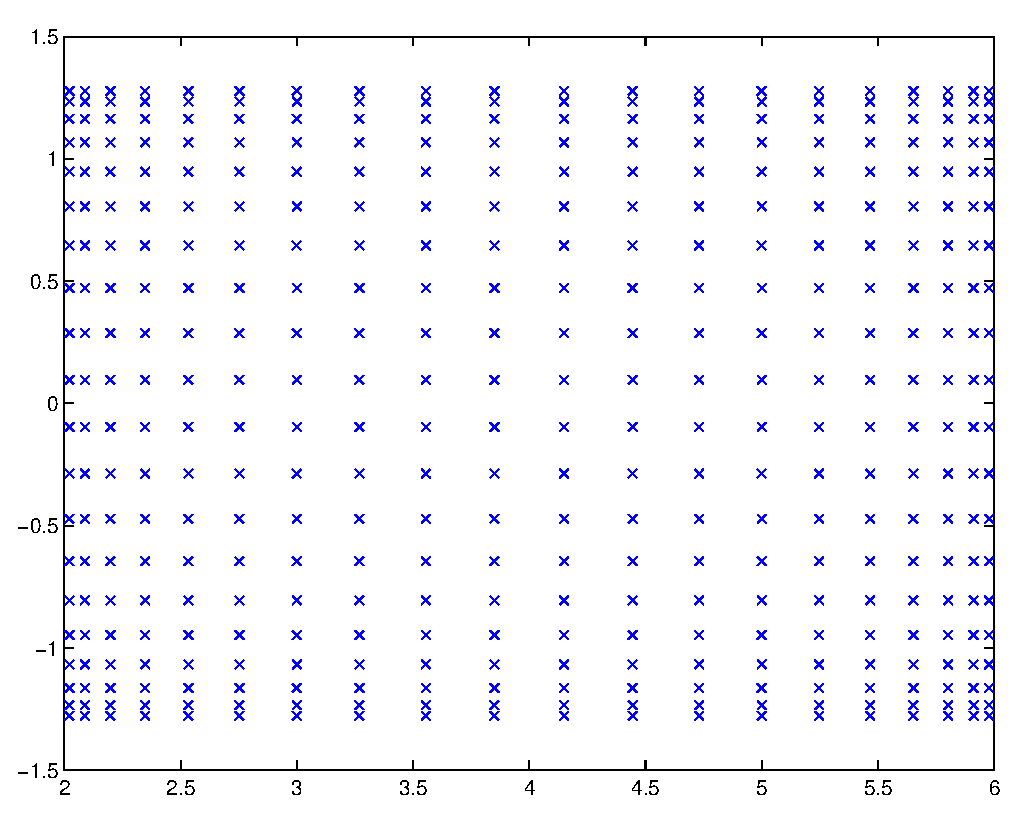
\includegraphics[scale=0.35]{eps/speke50n20.eps}
\hfill
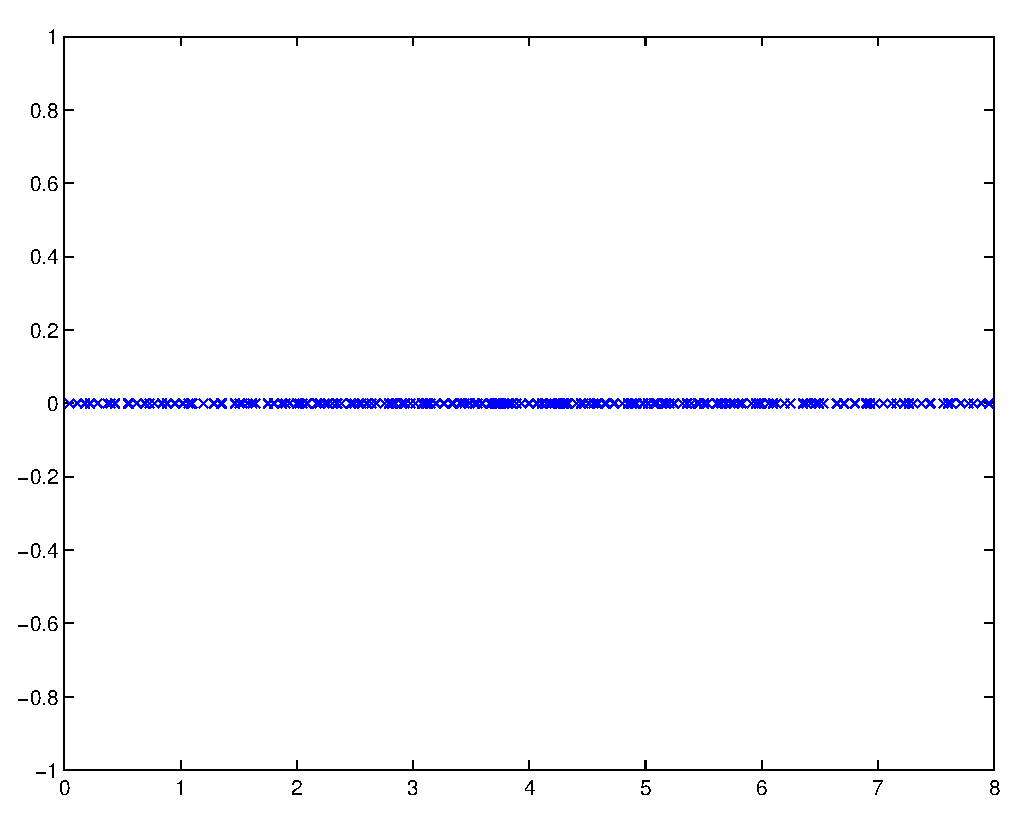
\includegraphics[scale=0.35]{eps/speke1n20.eps}
\caption{Spektrum von $A_{\epsilon}$ f"ur $N=20$ und $\epsilon = 50$ (links)
und $\epsilon = 1$ (rechts)}
\end{figure}

\begin{figure}
\includegraphics[scale=0.35]{eps/mp3e50n20k1.eps}
\hfill
\includegraphics[scale=0.35]{eps/mp3e1n20k1.eps}
\\
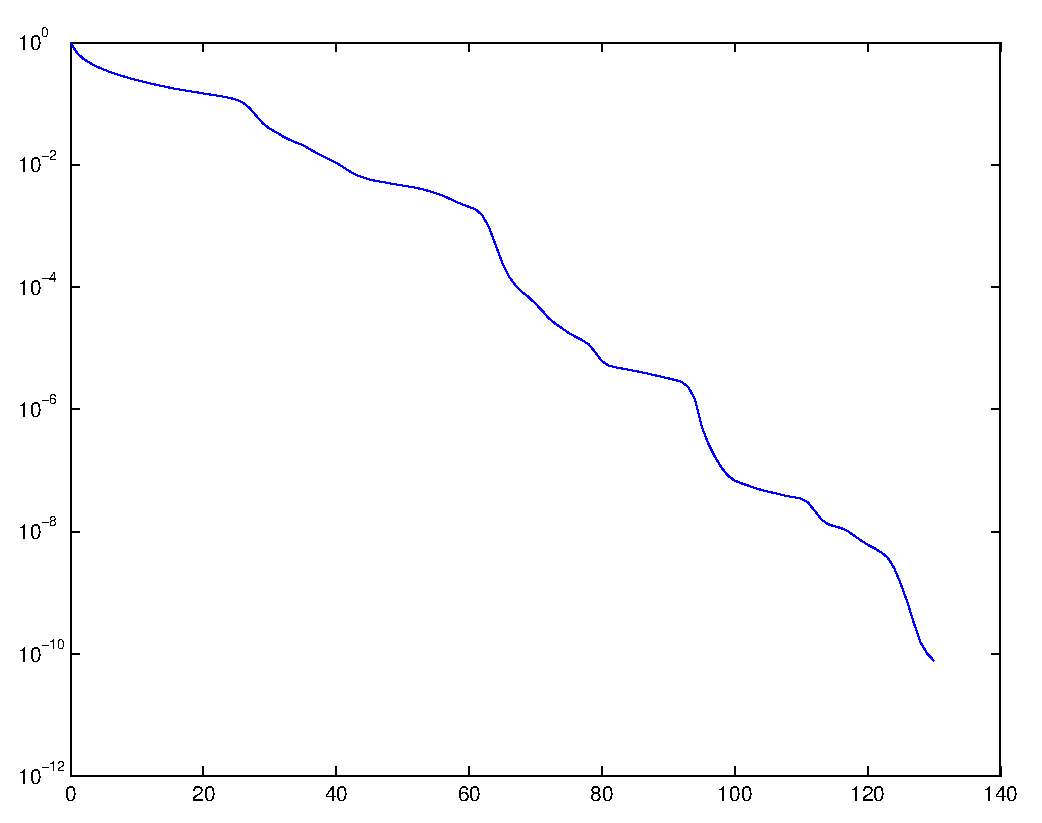
\includegraphics[scale=0.35]{eps/mp3e50n20k16.eps}
\hfill
\includegraphics[scale=0.35]{eps/mp3e1n20k16.eps}
\\
\includegraphics[scale=0.35]{eps/mp3e50n20k64.eps}
\hfill
\includegraphics[scale=0.35]{eps/mp3e1n20k64.eps}
\caption{Konvergenzgeschichte (Norm des Residuums als Funktion der 
Iterationszahl) f"ur GMRES($k$), $k=1,16,64$). Linke Spalte:
$N=20, \epsilon = 50$, rechte Spalte: $N=20, \epsilon = 1$}
\end{figure}


Spezialfall f\"ur GMRES: $A=A^H$, aber nicht notwendig hpd. 
Dann: Arnoldi- wird zum Lanczos-Prozess, d.h. kurze Rekursionen werden m\"oglich.
\begin{eqnarray*}
 H_{m+1,m} \rightarrow T_{m+1,m}=
 \left(\begin{array}{cccc}
                        \alpha_1  & \beta_2  & & \\
                        \beta_2   & \alpha_2 & \ddots  & \\
                                  & \ddots   & \ddots  & \beta_m \\
                                  &          & \beta_m & \alpha_{m} \\
					    &          &         & \beta_{m+1}
               \end{array}\right). 
\end{eqnarray*}
Die Berechnung der QR-Faktorisierung von $T_{m+1,m}$ vereinfacht sich:
\begin{eqnarray*}
 J_{m-1}^{(m+1)}\cdots J_{1}^{(m+1)} \cdot T_{m+1,m} & = &
 J_{m-1}^{(m+1)}\cdots J_{1}^{(m+1)} \cdot
               \left(\begin{array}{cc}
                        & 0\\
                        & \vdots\\
				& 0 \\
                        \raisebox{12pt}[-12pt]{\large $T_{m,m-1}$} & \beta_m \\
				& \alpha_m \\
				0 \ldots 0 & \beta_{m+1}
               \end{array}\right) \\
& = & \left(\begin{array}{cc}
                        & 0\\
                        & \vdots\\
				& 0 \\
				& \tilde \gamma_m \\
\quad                        \raisebox{12pt}[-12pt]{\large $R_{m,m-1}$} \quad& \tilde \beta_m \\
				& \tilde {\tilde \alpha}_m \\
				0 \cdots 0 & \beta_{m+1}
               \end{array}\right) 
\end{eqnarray*}
mit
\begin{eqnarray*}
 \tilde \gamma_m &=& \overline{s}_{m-2} \beta_m, \\
 \tilde{\tilde{\beta}}_m &=& c_{m-2} \beta_m, \\
 \tilde \beta_m &=& \overline{c}_{m-1} \tilde {\tilde{ \beta}}_m + \overline{s}_{m-1} \alpha_m, \\
 \tilde {\tilde \alpha}_m &=& -s_{m-1} \tilde {\tilde{ \beta}}_m + c_{m-1} \alpha_m.
\end{eqnarray*}
Setze nun
\begin{eqnarray*}
  {\tilde{ \alpha}}_m &=& \sqrt{|\tilde{ \tilde \alpha}_m|^2+|\beta_{m+1}|^2}, \\
 c_m &=&  \tilde {\tilde \alpha}_m /  {\tilde{ \alpha}}_m, \\
 s_m &=& \beta_{m+1} / {\tilde {\alpha}}_m.
\end{eqnarray*}
Mit
\begin{eqnarray*}
J_m^{(m+1)} = \left(\begin{array}{ccc}
                        & & \\
                        \raisebox{12pt}[-12pt]{\large I} & \raisebox{12pt}[-12pt]{\large 0}& \\
				& \overline{c}_m & \overline{s}_m \\
\raisebox{12pt}[-12pt]{\large 0}				& -s_m & c_m
               \end{array}\right) 
\end{eqnarray*}
gilt
\begin{eqnarray*}
 J_m^{(m+1)}\cdots J_1^{(m+1)} \cdot T_{m+1,m} &=&  
\left(\begin{array}{cc}
                        & 0\\
                        & \vdots\\
				& 0 \\
				& \tilde \gamma_m \\
\quad                        \raisebox{12pt}[-12pt]{\large $R_{m,m-1}$}\quad & \tilde \beta_m \\
				&  {\tilde {\alpha}}_m \\
				0 \cdots 0 & 0
               \end{array}\right) \; = \; R_{m+1,m}.
\end{eqnarray*}
$R_{m,m+1}$ hat nur drei besetzte Diagonalen.
Die GMRES-Iterierte $x^m$ erf\"ullt
$$ x^m = x^0 + V_m z^m \text{ mit } R_m z^m=\beta_1 (\epsilon_1,\ldots,\epsilon_m)^T .$$
Frage: Wie datiert man $x^m$ aus $x^{m-1}$ auf, wenn m"oglich mit kurzer Rekursion?

Es ist\begin{align*}
x^m&=x^0+V_mz^m\text{ mit }R_mz^m =\beta_1(\epsilon_1,\ldots,\epsilon_m)^T,
\intertext{also}
x^m&=x^0+\underbrace{V_mR_m^{-1}}_{=:W_m}\beta_1(\epsilon_1,\ldots,\epsilon_m)^T,
\end{align*}
mit $W_m=[w^1|\ldots|w^m]$. Wir setzen also
\begin{alignat*}{4}
&&W_m&=V_mR_m^{-1}\\
\iff&&W_mR_m&=V_m.
\end{alignat*}
Jetzt suchen wir eine Vorschrift zur Aufdatierung von $W_m$:\begin{alignat*}{4}
&&W_{m+1}R_{m+1}=V_{m+1}\\\\
\iff&&W_{m+1}
\left(\begin{array}{cc}
R_m&\begin{array}{c}
0\\\vdots\\0\\\tilde \gamma_{m+1}\\\tilde \beta_{m+1}
\end{array}\\
\begin{array}{ccc}
0&\ldots&0
\end{array}&\tilde\alpha_{m+1}
\end{array}\right)
&=[V_m|v^{m+1}]\\\\
\Longrightarrow\;&&W_{m+1}=[W_m|w^{m+1}]
\end{alignat*}
mit $\tilde\alpha_{m+1}w^{m+1}+\tilde\beta_{m+1}w^m+\tilde\gamma_{m+1}w^{m-1}=v^{m+1}$, also
\begin{equation}\label{wm+1_eq}
w^{m+1}=\frac{1}{\tilde \alpha_{m+1}}\left(v^{m+1}-\tilde\beta_{m+1}w^m-\tilde\gamma_{m+1}w^{m-1} \right).
\end{equation}
Damit erhalten wir
\begin{align*}
x^{m+1}&=x^0+W_{m+1}\beta_1(\epsilon_1,\ldots,\epsilon_{m+1})^T\\
&=x^0+W_{m}\beta_1(\epsilon_1,\ldots,\epsilon_m)^T+w^{m+1}\epsilon_{m+1}\beta_1\\
&=x^m+w^{m+1}\epsilon_{m+1}\beta_1.
\end{align*}
Somit ergibt sich die GMRES-Variante f\"ur hermitesche Matrizen.

\clearpage

\begin{alg}[MINRES, Paige\&Saunders, 1975]
~
\vspace*{-2\baselineskip}
\begin{algorithm}
\begin{algorithmic}
\STATE w\"ahle $x^0$, setze $r^0=b-Ax^0,\ \beta_1=\|r^0\|_2,\ v^1=\frac{1}{\beta_1}r^0$
\FOR{$m=1,2,\ldots$ bis $\|r^m\|$ klein genug}
\STATE bestimme $v^{m+1}$ aus dem Lanczos-Prozess
\STATE bestimme $\epsilon_{m+1},\tilde\gamma_{m+1},\tilde\beta_{m+1},\tilde\alpha_{m+1}$
\STATE bestimme $c_m,s_m$ gem\"a\ss \eqref{rotparam_eq}\hfill\COMMENT{alles kurze Rekursionen}
\STATE bestimme $w^{m+1}$ aus \eqref{wm+1_eq}
\STATE setze $x^{m+1}=x^m+\beta_1 \epsilon_{m+1}w^{m+1}$
\ENDFOR
\end{algorithmic}
\end{algorithm}
\end{alg}

\bigskip

Wie kann man die kurzen Rekursionen im Fall $A\ne A^H$ beibehalten?

\textbf{Idee:} Arbeite genau wie im MINRES-Verfahren, wobei diesmal $T_{m+1,m}$ durch den unsymmetrischen
Lanczos-Prozess geliefert wird (benutze dabei eine Variante, welche $\|v^j\|_2=1 $ liefert). Es gilt dann also
\[
x^m=x^0+V_mz^m
\]
mit $z^m$ l\"ost
\[
\min\|\beta_1e^1-T_{m+1,m}z^m\|_2,\; \beta_1=\|r^0\|_2.
\]

\begin{aufg}
Formuliere das unsymmetrische Lanczos-Verfahren \ref{unsymmetrisches Lanczos-Verfahren} so um, dass
$\|v^m\|_2=1$ f\"ur alle $m$ gilt.
\end{aufg}

Klar: $z^m$ und $x^m$ berechnen sich algorithmisch \emph{genau gleich} wie in MINRES. Wir verzichten deshalb auf ein explizites Aufschreiben. Was kann man jetzt "uber die Iterierte $x^m$ sagen?
\begin{align*}
\|b-Ax^m\|_2&=\|r^0-AV_mz^m\|_2\\
&=\|r^0-V_{m+1}T_{m+1,m}z^m\|_2\\
&=\|V_{m+1}(\beta_1e^1-T_{m+1,m}z^m)\|_2\\
&\le\underbrace{\|V_{m+1}\|_2}_{\le\sqrt{m+1}}\cdot\underbrace{\|\beta_1e^1-T_{m+1,m}z^m\|_2}_{\text{wird minimiert}}.
\end{align*}
Dieses Verfahren hei\ss t QMR ("`Quasi Minimal Residual"', Freund\& Nachtigal, 1990).

Eigenschaften sind:
\begin{itemize}
\item kurze Rekursionen
\item jeder Schritt erfordert zwei Matrix-Vektor-Multiplikationen (eine mit $A$, eine mit $A^H$; doppelter Aufwand wie bei GMRES)
\item Quasi-Minimierungseigenschaft:

Statt
\[
\|V_{m+1}(\beta_1e^1-T_{m+1,m}z^m)\|_2
\]
wird
\[
\|\beta_1e^1-T_{m+1,m}z^m\|_2
\]
minimiert.
\end{itemize}

\begin{aufg}
F\"uhre QMR aus f\"ur das lineare Gleichungssystem wie in Aufgabe \ref{GMRES_auf} und vergleiche mit
GMRES($k$) (Konvergenzgeschichte plotten).
\end{aufg}
\begin{figure}[h!]
\includegraphics[scale=0.35]{eps/mp3qmrN20e50.eps}\hfill\includegraphics[scale=0.35]{eps/mp3qmrN20e1.eps}
\caption{Konvergenzgeschichte f"ur QMR. Links:$N=20, \epsilon = 50$, rechts $N=20, \epsilon = 1$}
\end{figure}


\section{Konvergenzanalyse f�r GMRES/MINRES}

Gegeben sei $A\in\cnn,\ Ax=b,\ A$ regul�r.

\begin{defn}
Der \emph{numerische Wertebereich} von $A$ ("`fields of value"') ist definiert durch
\begin{align*}
F(A)&=\left\{\frac{\langle Ax,x\rangle}{\langle x,x\rangle}:\ x\in \cn,\ x\ne 0 \right\}\\
&=\left\{\langle Ax,x\rangle:\ \|x\|_2=1 \right\}.
\end{align*}
\end{defn}

Mit elementarer Rechnung ergeben sich die folgenden Eigeschaften des numerischen Wertebereichs:
\begin{lem}
\begin{enumerate}
\item Ist $A$ hermitesch mit spek$(A)=\{\lambda_1\le\ldots\le\lambda_n\}$, dann ist $F(A)=[\lambda_1,\lambda_n]$.
\item spek$(A)\subseteq F(A)$.
\item Ist $A$ normal, dann ist $F(A)=$co(spek$(A)$) (co$(M)$ = konvexe H�lle von $M$).
\end{enumerate}
\end{lem}

\begin{sa}
\begin{enumerate}
\item Der numerische Wertebereich $F(A)$ ist kompakt, also ist der \emph{numerische Radius}
\[
r(A):=\sup \{|\lambda|:\ \lambda\in F(A)\}
\]
endlich (und das $\sup$ ist ein $\max$).
\item $F(A)$ ist konvex.
\end{enumerate}
\end{sa}
\begin{proof}
\begin{enumerate}
\item Klar.
\item Das ist etwas weniger selbstverst\"andlich. Sei $\lambda, \mu \in F(A)$, $\lambda \neq \mu$. Wir zeigen, dass $\eta(t) =t\lambda +(1-t) \mu \in F(A)$ f�r alle $t \in [0,1]$. Man beachte, dass gilt
\[
\eta(t) \in F(A) \Leftrightarrow t \in F(\underbrace{\alpha I+\beta A}_{ =: S}) \text{ mit } \alpha = -\frac{\mu}{\lambda-\mu}, \beta = \frac{1}{\lambda-\mu}.
\]
Wir zeigen deshalb, dass $[0,1] \in F(S)$.
Sei nun $\lambda = \langle Ax, x \rangle, \mu = \langle Ay, y \rangle$ with $\|x\|= \|y\|=1$.
Eine einfache Rechnung ergibt
\[
\langle Sx, x \rangle =1, \langle Sy, y \rangle=0.
\]
Definiere $g:\mathbb{R} \to \mathbb{C}$ mit $\theta \mapsto g(\theta)= \langle Sy,x\rangle e^{-i\theta}+ \langle Sx,y \rangle e^{i\theta}$. Offensichtlich ist $\Im(g(0))= -\Im(g(\pi))$. Weil $g$ und damit $\Im(g)$ stetig ist, existiert $\theta_0 \in [0,\pi]$ mit $\Im(g(\theta_0))=0$.

Wegen $\lambda \neq \mu$ sind die Vektoren $y$ und $\hat x = e^{i\theta_0}x$ linear unabh\"angig. Also gilt $z(t) = t \hat x + (1-t)y \neq 0$ f\"ur alle $t$ und wir bezeichnen mit $\hat z(t)$ ihre auf 1 normierte Versionen. Die Funktion $f(t) = \langle S \hat z(t), \hat z(t)$ is stetig und reellwertig (!) auf $[0,1]$ mit $f(0) = 0, f(1) =1$. Also gilt $[0,1] \in F(S)$. Dies war zu zeigen.
\end{enumerate}
\end{proof}
\begin{bsp}Die Matrix $A$ aus Beispiel~\ref{stagnation_bsp} ist normal. Deshalb ist $F(A)$ die konvexe H"ulle der Eigenwerte, also hier ein (ausgef"ulltes) regelm"a"siges $n$-Eck im Einheitskreis.  \end{bsp}

\begin{aufg}Zeigen Sie, dass f"ur die Matrix \[A=\left(\begin{array}{cc}0&2\\0&0\end{array}\right)\] der numerische Wertebereich gegeben ist durch $F(A)=\{z\in\co:\ |z|\le 1\}$.\end{aufg}
\begin{lem}Sei $V_m\in\co^{n\times m},\ V_m^HV_m=I$. Dann gilt
\[
F(V_m^HAV_m)\subseteq F(A).
\]
\end{lem}
Der Beweis ist wieder trivial.
 
\begin{sa}\label{GMRES_NST_sa}
Sei $p_m^{\text{GMRES}}$ das Residuen-Polynom aus dem GMRES-Verfahren, d.h. 
\[
r^m=p_m^{\text{GMRES}}(A)r^0, \quad p_m^{\text{GMRES}}\in\overline{\Pi} _m.
\]
Dann gilt 
\[
p_m^{\text{GMRES}}(\xi)=0\Rightarrow\frac{1}{\xi}\in F(W_m^HA^{-1}W_m)\subseteq F(A^{-1}).
\]
Dabei ist $W_m\in\co^{n\times m}$ eine Matrix, deren Spalten eine Orthonormalbasis von $A\cdot K_m(A,r^0)$ bilden.
\end{sa}
\begin{proof}
Setze $p_m:=p_m^{\text{GMRES}}$. Es ist
\begin{align*}
p_m(t)&=\prod\limits_{j=1}^m\left(1-\frac{t}{\xi_j} \right).
\intertext{Betrachte $\xi=\xi_m$:}
p_m(t)&=\left(1-\frac{t}{\xi} \right)\cdot q_{m-1}(t)\text{ mit } q_{m-1}(t)=\prod\limits_{j=1}^{m-1}\left(1-\frac{t}{\xi_j} \right).
\intertext{Damit ist}
\|p_m(A)r^0\|_2&=\|(I-\frac{1}{\xi}A)\cdot \underbrace{q_{m-1}(A)\cdot r^0}_{w}\|_2
\end{align*}
minimal. Also ist $\xi$ so, dass $\|(I-\frac{1}{\xi}A)w\|_2$ minimal ist.
Nach Lemma~\ref{minimierungs_lem} (s. unten) gilt deshalb
\[
\frac{1}{\xi}=\frac{\langle w,Aw\rangle}{\langle Aw,Aw\rangle}=\frac{\langle A^{-1}y ,y\rangle}{\langle y,y\rangle}
\]
mit $y=Aw\in A\cdot K_m(A,r^0)$.
\end{proof}

\begin{lem} \label{minimierungs_lem}
Die L"osung von $\underset{\gamma}{\min}\|w-\gamma y\|_2$ ist
\[
\gamma^*=\frac{\langle w,y\rangle}{\langle y,y\rangle}
\]
\end{lem}
%{\bf Beweis:}
\begin{proof}
Es ist
\begin{align*}
\langle w-\gamma y,w-\gamma y\rangle&=\langle w,w\rangle-\gamma \langle y,w\rangle
						-\bar \gamma \langle w,y\rangle+\gamma\bar \gamma\langle y,y\rangle\\
&=\langle w,w\rangle+\langle y,y\rangle\left(\gamma\bar\gamma-\frac{\langle y,w\rangle}{\langle y,y\rangle}\gamma 
						-\frac{\langle w,y\rangle}{\langle y,y\rangle}\bar \gamma\right.\\
&\hspace*{4cm}\left.				+\frac{\langle y,w\rangle\langle w,y\rangle}{\langle y,y\rangle^2}\right)
						-\frac{\langle y,w\rangle\langle w,y\rangle}{\langle y,y\rangle}\\
&=\langle w,w\rangle+\langle y,y\rangle\left(\gamma-\frac{\langle w,y\rangle}{\langle y,y\rangle} \right)
					    \left(\bar \gamma-\frac{\langle y,w\rangle}{\langle y,y\rangle} \right)\\
&\hspace*{7cm}	-\frac{\langle y,w\rangle\langle w,y\rangle}{\langle y,y\rangle}.
\end{align*}
Das Minimum wird also f�r
\[
\gamma ^*=\frac{\langle w,y\rangle}{\langle y,y\rangle}
\]
erreicht.
%}
\end{proof}

Schr�nken wir $A\in\co^{n\times n}$ auf einen Unterraum $V \subseteq \co^n$ ein, so ist nicht
notwendig $AV \subseteq V$. M�chte man einen Homomorphismus auf $V$, muss man $AV$ geeignet
projizieren.

\begin{defn}Die {\em orthogonale Projektion} von $A \in \co^{n \times n}$ auf den Unterraum
 $V \subseteq \co^n$ entsteht durch
orthogonale Projektion von $AV$ auf $V$. Bilden die Spalten von
$ V_m\in\co^{m\times n}$ eine Orthonormalbasis von $V$  ($V_m^HV_m=I$), so ist
$V_m^HAV_m$ die Darstellung der orthogonalen Projektion von $A$ auf $V$
in der Basis "`Spalten von $V_m$"'.
\end{defn}

\begin{sa}\label{GMRESabschaetz_sa}
Es sei $0\notin F(A)$ und $c:=\min\{|\lambda|:\ \lambda\in F(A)\}>0$. Dann ist $c \leq \|A\|_2$
und es gilt
\begin{equation} \label{gmres_konv_sa}
\|p_m^{\text{GMRES}}(A)r^0\|_2\le \left(1-\textstyle\frac{c^2}{\|A\|_2^2} \right)^{\textstyle\frac{m}{2}}\cdot \|r^0\|_2.
\end{equation}
\end{sa}
\begin{proof} Es ist
\[
c \le \frac{| \langle Aw,w\rangle|}{\langle w,w \rangle} \leq
 \frac{ \|Aw\|_2 \cdot \|w\|_2}{\langle w,w \rangle} \leq
\frac{ \|A\|_2  \cdot \|w\|_2^2}{\langle w,w \rangle} = \|A\|_2.
\]

Zum Beweis von \eqnref{gmres_konv_sa} starten wir mit einer
Vor�berlegung.
Nach Lemma~\ref{minimierungs_lem} gilt f�r $\frac{1}{\xi} =
\frac{\langle w, Aw\rangle}{\langle Aw,Aw \rangle}$
\[
\langle w-\textstyle\frac{1}{\xi}Aw,w-\textstyle\frac{1}{\xi}Aw\rangle
=\langle w,w\rangle-\textstyle\frac{\langle Aw,w\rangle\langle w,Aw\rangle}{\langle Aw,Aw\rangle} .
\]
F�r $w\ne 0$ gilt au�erdem
\begin{align*}
\langle Aw,Aw\rangle&=\|Aw\|_2^2\le \|A\|_2^2\cdot \langle w,w\rangle,\\
|\langle Aw,w\rangle|^2&\ge \left|\textstyle\frac{\langle Aw,w\rangle}{\langle w,w\rangle} \right|^2\cdot \langle w,w\rangle^2\\
&\ge c^2\cdot \langle w,w\rangle^2.
\end{align*}
Also ist f�r die angegebene Wahl von $\xi$
\begin{equation} \label{absch1_eq}
\langle w-\textstyle\frac{1}{\xi}Aw,w-\textstyle\frac{1}{\xi}Aw\rangle\le  \left(1-\textstyle\frac{c^2}{\|A\|_2^2} \right)\cdot \langle w,w\rangle,
\end{equation}
mit $ \left(1-\textstyle\frac{c^2}{\|A\|_2^2} \right)\in[0,1)$.

\medskip
Wir schreiben wieder $p_m$ statt $p_m^{\text{GMRES}}$
und zeigen \eqnref{gmres_konv_sa} per Induktion.
\begin{Blist}{$m-1\to m$}
\item[\hfill $m=0$] klar.
\item[$m-1\to m$] F�r $w=p_{m-1}(A)r^0$ ist nach Induktionsvoraussetzung
\[
\|w\|_2\le \left(1-\textstyle\frac{c^2}{\|A\|_2^2} \right)^{\textstyle\frac{m-1}{2}}\cdot \|r^0\|_2.
\]
Auf Grund der Minimalit�tseigenschaft ist f�r alle $\xi\in\co\backslash\{0\}$
\[
\|p_m(A)r^0\|_2\le \|(I-\textstyle\frac{1}{\xi}A) p_{m-1}(A)r^0\|_2 = \|(I-\textstyle\frac{1}{\xi}A)w\|_2.
\]
Speziell f�r die Wahl $\textstyle\frac{1}{\xi}=\textstyle\frac{\langle w,Aw\rangle}{\langle Aw,Aw\rangle}$ ergibt sich nach \eqnref{absch1_eq}
\[
\left \|\left(I-\textstyle\frac{1}{\xi}A\right)w \right\|_2^2\le \left(1-\textstyle\frac{c^2}{\|A\|^2} \right) \cdot \|w\|_2^2.
\]
\end{Blist}
\end{proof}

\begin{bem}Der Beweis hat gezeigt, dass unter den Voraussetzungen von Satz \ref{GMRESabschaetz_sa} sogar gilt, dass GMRES($k$) f�r alle Restartwerte
$k$  mit der selben Absch�tzung \eqnref{gmres_konv_sa} konvergiert.
\end{bem}

Wir diskutieren die Nullstellen der GMRES-Polynome jetzt noch genauer.

\begin{lem}\label{GMRES_res_lem}
F�r die GMRES-Residuen
\[
r^m=p_m^{\text{GMRES}}(A)r^0
\]
gilt
\[
r^m\bot A\cdot K_m(A,r^0).
\]
(Zum Vergleich: Beim cg-Verfahren gilt $r^m \bot K_m(A,r^0)$.)
\end{lem}
\begin{proof}
Es gilt
\[
r^m=b-Ax^m=r^0-AV_mz^m, \quad z^m\in\co^m\text{ mit } \|r^0-AV_mz^m\|_2\text{ minimal.}
\]
Also erf�llt $z^m$ die Normalengleichung (s.\ Numerik I)
\[
\underbrace{V_m^HA^HAV_m}_{M_m}z^m=V_m^HA_m^Hr^0
\]
mit $M_m$ hpd, da $V_m$ vollen Rang besitzt. Also ist
\[
z^m=M_m^{-1}V_m^HAr^0
\]
und es gilt f�r alle $y\in\co^{m}$
\begin{align*}
\langle r^m,AV_my\rangle
&=\langle r^0-AV_mM_m^{-1}V_m^HA^Hr^0, AV_my\rangle\\
&=\langle r^0,AV_my\rangle-\langle r^0,AV_m\underbrace{M_m^{-1}V_m^HA^HAV_m}_{=I} y\rangle\\
&=0.
\end{align*}
\end{proof}

\begin{sa}
Die Nullstellen $\xi_i$ der GMRES-Polynome $p_m^{\text{GMRES}}$ sind Eigenwerte des verallgemeinerten
Eigenwertproblems
\begin{equation}
(H_{m+1,m}^HH_{m+1,m})\cdot z=\xi H_m^H \cdot z,\label{verallg_ewprob_eq}
\end{equation}
wobei $H_m$ aus $H_{m+1,m}$ durch Streichen der letzten Zeile entsteht.
\end{sa}
\begin{proof}
Man beachte, dass das Produkt $H_{m+1,m}^HH_{m+1,m}$  hpd ist, $H_m$ jedoch singul�r sein kann.
Sei 
\[
r^m=p_m(A)r^0=\left(I-\textstyle\frac{1}{\xi}A \right)\underbrace{q_{m-1}(A)r^0}_{= V_mz},\ p_m(\xi)=0.
\]
Nach Lemma \ref{GMRES_res_lem} gilt mit $AV_m = V_{m+1}H_{m+1,m}$
\begin{align*}
&r^m \bot AK_m(A,r^0)\\
\iff&\langle r^m,AV_my\rangle=0 \quad \forall\ y,\\
\iff&\langle (I-\xi^{-1}A)V_mz,AV_my\rangle =0 \quad \forall\ y, \\
\iff&\langle V_mz-\xi^{-1}V_{m+1}H_{m+1,m}z,V_{m+1}H_{m+1,m}y\rangle=0 \quad \forall\ y, \\
\iff&\langle V_mz,V_{m+1}H_{m+1,m}y\rangle-\xi^{-1}\langle V_{m+1}H_{m+1,m}z,V_{m+1}H_{m+1,m}y\rangle=0 \quad \forall\ y, \\
\iff&y^HH_{m+1,m}^HV_{m+1}^HV_mz-\xi^{-1}y^HH_{m+1,m}^H\underbrace{V_{m+1}^HV_{m+1}}_{=I}H_{m+1,m}z=0 \quad \forall\ y. \\
\intertext{Dabei ist $V_{m+1}^HV_m=\left(\begin{array}{c}
I_m\\
\begin{array}{ccc}
0&\ldots&0
\end{array}
\end{array}\right)$ und damit $H_{m+1,m}^HV_{m+1}^HV_m=H_m^H$. Wir erhalten also}
&r^m \bot AK_m(A,r^0)\\
\iff&y^H(H_m^Hz-\xi^{-1}H_{m+1,m}^HH_{m+1,m}z)=0\\
\iff&H_m^Hz-\xi^{-1}H_{m+1,m}^HH_{m+1,m}z=0.
\end{align*}
\end{proof}

\textbf{Bedeutung von \eqnref{verallg_ewprob_eq}:} Betrachte die orthogonale Projektion von $A^{-1}$ auf
$A\cdot K_m(A,r^0)$.
Eine ONB von $AK_m(A,r^0)$ sind die Spalten von
\[
AV_mM_m^{-\textstyle\frac{1}{2}} \quad \text{mit } M_m=V_m^HA^HAV_m,
\]
denn (Basis ist klar)
\[
M_m^{-\textstyle\frac{1}{2}}\underbrace{V_m^HA^HAV_m}_{M_m}M_m^{-\textstyle\frac{1}{2}}=I.
\]
Die orthogonale Projektion von $A^{-1}$ auf $AK_m(A,r^0)$ wird repr�sentiert durch
\begin{align*}
M_m^{-\textstyle\frac{1}{2}}V_m^H(A^HA^{-1}A)V_mM_m^{-\textstyle\frac{1}{2}}
&=M_m^{-\textstyle\frac{1}{2}}(AV_m)^HV_mM_m^{-\textstyle\frac{1}{2}}\\
&=M_m^{-\textstyle\frac{1}{2}}(V_{m+1}H_{m+1,m})^HV_mM_m^{-\textstyle\frac{1}{2}}\\
&=M_m^{-\textstyle\frac{1}{2}}H_m^HM_m^{-\textstyle\frac{1}{2}}.
\end{align*}
Damit ist $\xi^{-1}$ Eigenwert dieser orthogonalen Projektion, wenn
\begin{alignat*}{6}
&&M_m^{-\textstyle\frac{1}{2}}H_m^HM_m^{-\textstyle\frac{1}{2}}z&=\xi^{-1} z &&\quad \text{mit } z\ne 0\\
\iff&&H_m^Hy&=\xi^{-1}M_my &&\quad\text{mit } y=M_m^{-\textstyle\frac{1}{2}}z.
\end{alignat*}

\bigskip

Wir halten fest
\begin{sa}
$\xi$ ist Nullstelle von $p_m^{\text{GMRES}}$ genau dann, wenn $\xi^{-1}$ Eigenwert der orthogonalen Projektion von
$A^{-1}$ auf $A\cdot K_m(A,r^0)$ ist.
\end{sa}

Spezialfall: $A$ normal
\begin{eqnarray*} \begin{array}{lcl}
  \Rightarrow  A &=& Q^H \Lambda Q, \quad Q^H Q=I, \quad \Lambda =\diag(\lambda_1,\ldots,\lambda_n) \\
  \Rightarrow  A^{-1} &=& Q^H \Lambda^{-1} Q
\end{array} \end{eqnarray*}
Damit ist die orthogonale Projektion von $A^{-1}$ auf $AK_m(A,r^0)$ die Matrix
\begin{align*}
W_m^H A^{-1} W_m = W_m^H Q^H \Lambda^{-1}\underbrace{QW_m}_{\text{orthonormal}} =:B \in \cmm
\end{align*}
mit $W_m^HW_m=I,W_m\in\cnm$.
$B$ ist selbst normal, $B=P^HD_mP, P\in\cmm$ orthonormal, $D_m=\diag(d_1,\ldots,d_m)$. \\ Also
\begin{eqnarray*}
 & P^HD_mP &= W_m^HQ_m^H\Lambda^{-1}QW_m \\
\Leftrightarrow & D_m &= (PW_m^HQ_m^H)\Lambda^{-1}(\underbrace{QW_mP^H}_{=:Y}) \\
\Rightarrow & d_i &= \sum\limits_{j=1}^n \frac{1}{\lambda_i} |y_{ji}|^2  \quad \text{mit}
\sum\limits_{j=1}^n |y_{ji}|^2 =1.\end{eqnarray*}
$\frac{1}{\xi}$ ist einer der Eigenwerte $d_i$ von $B$. Also haben wir
\begin{sa}
Ist $A$ normal (z.B. $A=A^H$), so sind die Nullstellen der GMRES-Polynome gewichtete harmonische Mittel
der Eigenwerte von $A$, d.h.
$$ p_m^{\text{GMRES}}(\xi)=0 \Rightarrow \frac{1}{\xi}=\sum\limits_{j=1}^n\alpha_j \frac{1}{\lambda_j} $$
mit $\alpha_j>0,\sum\alpha_j=1,\lambda_j$ Eigenwerte von A.
\end{sa}
Man nennt die $\xi$ deshalb auch {\em harmonische Ritz-Werte}.
\begin{bem}
$A$ sei hermitesch, $spek(A)\cap[-b,a]=\emptyset,a,b>0$. Dann folgt $\xi\notin[-b,a]$.
\end{bem}
Spezielle Resultate f"ur MINRES:
\begin{sa}
Sei $A=A^H \in\cnn$ regul"ar, $\lambda_1 \leq \lambda_2 \leq \ldots \leq \lambda_{n^*}$ seien die
verschiedenen Eigenwerte von $A$, $n^*\leq n$.
\begin{enumerate}
\item Es gelte $\lambda_1 \leq \ldots \leq \lambda_k < 0$ und $\lambda_{k+1}>0$.
      Dann gilt f"ur das Verfahren MINRES
	\begin{eqnarray*}
	\|r^{m+k}\|_2 \leq \frac{2c^m}{1+c^{2m}}\prod_{i=1}^k           \left(1-\frac{\lambda_{n^*}}{\lambda_i}\right)\|r^0\|_2
      \end{eqnarray*}
	mit $c=\frac{\sqrt{\kappa}-1}{\sqrt{\kappa}+1} \text{ und } \kappa=\frac{\lambda_{n^*}}{\lambda_{k+1}}$
\item Es gelte $\spek(A)\subseteq[-b,-a]\cup[a,b],0<a\leq b$. Dann gilt f"ur das Verfahren MINRES
	\begin{eqnarray*}
	\|r^{2m}\|_2 \leq \frac{2\tilde c^m}{1+\tilde c^{2m}}\|r^0\|_2
	\end{eqnarray*}
	mit $\tilde c=\frac{\tilde \kappa-1}{\tilde \kappa+1} \text{ und } \tilde \kappa=\frac{b}{a}$
\end{enumerate}
\end{sa}
\begin{proof}
Zu 1.: Nehme
\begin{eqnarray*}
p_{m+k}(t)=\prod_{i=1}^k \left(1-\frac{t}{\lambda_i}\right) \cdot T_m^{[\lambda_{k+1},\lambda_{n^*}]}(t)
\end{eqnarray*}
mit $T_m^{[\lambda_{k+1},\lambda_{n^*}]}$ Tschebyscheff-Polynom f"ur $[\lambda_{k+1},\lambda_{n^*}]$.
Dann gilt mit Korollar~\ref{Tscheb_pos_def_cor}
\begin{eqnarray*}
\max_{t\in \spek(A)}|p_{m+k}(t)| &=& \max\limits_{t\in[\lambda_{k+1},\lambda_{n^*}]}|p_{m+k}(t)| \\
 &\leq& \frac{2c^m}{1+c^{2m}}\prod\limits_{i=1}^k\left(1-\frac{\lambda_{n^*}}{\lambda_i}\right). \\
\end{eqnarray*}
Damit gilt
\begin{eqnarray*}
\|r^{m+k}\|_2 &=& \|p_{m+k}^{\text{MINRES}}(A)r^0\|_2 \\              & \leq & \|p_{m+k}(A)r^0\|_2 \\
 &\leq& \|p_{m+k}(A)\|_2\cdot\|r^0\|_2 \\
 &=& \max_{t\in \spek(A)}|p_{m+k}(t)|\cdot\|r^0\|_2 \\
 &\leq&  \frac{2c^m}{1+c^{2m}}\cdot\prod_{i=1}^k\left(1-\frac{\lambda_{n^*}}{\lambda_i}\right)\cdot\|r^0\|_2.
\end{eqnarray*}

Zu 2.: Nehme $p_{2m}(t)=T_m^{[a^2,b^2]}(t^2)$. Dann gilt
\begin{eqnarray*}
\|r^{2m}\|_2 &\leq& \|T_m^{[a^2,b^2]}(A^2)\|_2\cdot\|r^0\|_2 \\
 &\leq& \max_{s\in \spek(A^2)}|T_m^{[a^2,b^2]}(s)|\cdot\|r^0\|_2 \\
 &\leq& \max_{s\in [a^2,b^2]}|T_m^{[a^2,b^2]}(s)|\cdot\|r^0\|_2 \\
 &=& \frac{2 \tilde c^m}{1+\tilde c^{2m}}\cdot\|r^0\|_2
\end{eqnarray*}
\end{proof}
\begin{bem}
Im 1. Fall ist f"ur kleines $k$ die Konvergenz von MINRES also vergleichbar mit CG
(auf $[\lambda_{k+1},\lambda_{n^*}]$). CG f"ur $A^HAx=A^Hb$ mit $A^HA$ hpd ben"otigt:
2 MVM pro Schritt (A und $A^H$) und $$\kappa(A^HA)=
\frac{\max\{\lambda_1^2,\lambda_{n^*}^2\}}{\min\{\lambda_k^2,\lambda_{k+1}^2\}}\geq \kappa^2.$$
Wenn $k$ klein ist, ist CG f"ur $A^HA$ also 4-mal so aufwendig. \medskip

Vergleich mit CG im 2. Fall, wobei $a$ und $b$ jetzt beide Eigenwerte von $A$ seien. \\
Wegen $\kappa(A^HA)=\frac{b^2}{a^2}$ folgt dann: CG f"ur $A^HA$ ist gleich schnell wie MINRES.
\end{bem}
Der Fall $\spek(A)\subseteq[-b,-a]\cup[c,d]$ kann allgemein mit Orthogonalpolynomen bzgl.
zueinander disjunkter Intervalle behandelt werden.\\
Siehe dazu: Bernd Fischer - Polynomial Based Iteration Methods for Symmetric
Linear Systems, Wiley (1995).
\section[FOM und CG]{FOM und CG}
{\bf Gegeben: }
\begin{quote}
$Ax=b$, $A \in \cnn$, $A$ regul"ar.
\end{quote}
{\bf Gesucht: }
\begin{quote}
$r^m\in K_m(A,r^0)$, s.d.
\begin{equation} \label{galbed}
r^m \perp K_m(A, r^0).
\end{equation}
\end{quote}
\eqref{galbed} hei"st \textsl{Galerkin}-Bedingung. \\
Erinnerung an Arnoldi-Verfahren:
\begin{equation} \label{arnoldi_relation}
\begin{array}{rcl}
AV_m &=& V_{m+1}H_{m+1,m} 
\end{array} 
\end{equation}
mit
\begin{eqnarray*}
 H_{m+1,m}=
 \left(\begin{array}{c} 
                H_m \\
                h_{m+1,m}e_m^T
               \end{array}\right), \quad H_m \in \mathbb{C}^{m \times m}.
\end{eqnarray*}

\begin{sa} \label{sa:FOM_ber} $x \in x_0 + K_m(A,r^0)$ ef�llt die Galerkin-Bedingung \eqref{galbed} genau dann, wenn $x = x^m = x^0 + V_mz^m$ mit 
\begin{equation} \label{eq:z_fuer_Galerkin}
H_mz^m = \beta_0 e_1, \enspace \beta_ 0 = \|r^0\|.
\end{equation}
Das zugeh"orige Residuum $r^m$ ist ein skalares Vielfaches von $v^{m+1}$.
\end{sa}
\begin{proof} F"ur $x = x^0 + V_mz$ mit $z \in \mathbb{C}^m$ gilt
\begin{eqnarray*}
& & b-Ax \perp K_m(A,r^0) \\
&\Leftrightarrow & r^0 - AV_m^ \perp K_m(A,r^0)\\
&\Leftrightarrow & V_m^H(r^0-AV_mz) = 0 \\
&\Leftrightarrow & \beta_0e_1 - H_m z = 0 \\
&\Leftrightarrow & z = z_m \text{ aus \eqref{eq:z_fuer_Galerkin}} 
\end{eqnarray*}
Weiterhin ist $r^m = b-Ax^m = r^0 - AV_mz^m \in K_{m+1}(A,r^0)$ und $r^m \perp K_m(A,r^0)$. Das orthogonale Komplement von $K_m(A,r^0)$ in $K_{m+1}(A,r^0)$ wird nach Konstruktion der Arnoldi-Vektoren aber gerade von $v^{m+1}$ aufgespannt. 
\end{proof}

\subsection{FOM}

\begin{defn} Die Full Orthogonalization Method (FOM) ist das Krylov-Unteraumverfahren, dessen Iterierte \eqref{galbed} erf"ullen, die sich also gem"a� Satz~\ref{sa:FOM_ber} berechnen.
\end{defn}


\begin{alg}[FOM]
~               % um "Algorithmus" aus dem Kasten rauszubekommen
\vspace*{-2\baselineskip}       % um den Leeraum zu entfernen
\begin{algorithm}
  \begin{algorithmic}
    \STATE w\"ahle $x^0$, setze $r^0 = b-Ax^0$, $\beta_0 = \|r^0\|$, $v^1 = \frac{1}{\beta_0}r^0$
    \FOR{$m = 1,2 \dots$ }
      \STATE bestimme den n"achsten Arnoldi-Vektor, dies ergibt die Arnoldi-Relation auf Stufe $m$: $AV_m = V_{m+1}H_{m+1,m}$ 
      \STATE setze $x^m = x^0 + \beta_0 H_m^{-1}e_1 $
    \ENDFOR
  \end{algorithmic}
\end{algorithm}
\end{alg}

\begin{bem} Die FOM Iterierten brauchen nicht alle zu existieren, weil $H_m$ singul"ar werden kann. 
\end{bem}

\begin{bsp} Sei
\[
A = \left( \begin{array}{cc} 1 & 0 \\ 0 & -1 \end{array} \right) \text{ und } r^0 = \left( \begin{array}{c} 1 \\ 1 \end{array} \right).
\]
Dann ist $v_1 = \frac{1}{\sqrt{2}}r^0$ und $H_1 = 0 \in \mathbb{C}^{1 \times 1}$. Die FOM-Iterierte $x^1$ existiert also nicht. \\
Beachte: $A$ in diesem Beispiel ist sogar symmetrisch.
\end{bsp}




\begin{aufg} \label{aufg:fom_existenz}  Zeige: Falls $0 \not \in F(A)$, so ist $H_m$ nicht-singul"ar f"ur alle $m$. 
\end{aufg}

FOM f"ur allgemeines $A$ erfordert wie GMRES die Speicherung alle Arnoldi-Vektoren und der Aufwand pro Schritt erh"oht sich mit $m$. Im Gegensatz zu GMRES ist die Galerkin-Bedingung keine Minimalit"atsbedingung $\Longleftrightarrow$ das Verhalten von Fehler und Residuum ist nicht monoton, es kann starke Ausschl"age geben.  

Wenn $A$ aber hpd ist, so kann die Galerkin-Bedingung als Minimalit"atsbedingung interpretiert werden. Weil dann Arnoldi zu Lanczos wird, kann ein Verfahren mit kurzer Rekursion formuliert werden: CG.

\subsection{CG}
\begin{lem} \label{lem:min} Sei $B \in \mathbb{C}^{m \times m}$ hpd, $a \in \mathbb{C}^m$. Dann wird
\[
f(x) = \langle Bx,x\rangle - 2 \Re \langle x,a \rangle 
\]
minimal auf $\mathbb{C}^m$ f"ur $x = x^*=B^{-1}a$. 
\end{lem}
\begin{proof} Es ist
\[
f(x = \underbrace{\langle B(x-B^{-1}a), x- B^{-1}a \rangle}_{ \geq 0, \, =0 \text{ f"ur } x = x^*} - \langle B^{-1}a,B^{-1}a \rangle.
\]
\end{proof}



\begin{sa} $A$ sei hpd. Dann erf"ullt $x^m \in x^0 + K_m(A,r^0)$ die Galerkin-Bedingung \eqref{galbed} genau dann, wenn $x^m$ den Fehler in der $A$-Norm minimiert,
\[
x^m = \mbox{argmin}_{x \in x^0 + K_m(A,r^0)} \|A^{-1}b - x \|_A,
\]
wobei $\| y \|_A := \langle Ay,y\rangle^{1/2}$.
\end{sa}
\begin{proof} Sei $x = x^0 + V_m z$. Wir bezeichnen $e^0 = A^{-1}r^0 = A^{-1}b-x^0$. Dann ist
\begin{eqnarray*}
\|A^{-1}b -x \|_A^2 &=& \langle b-Ax, A^{-1}b-x \rangle \\
& = & \langle r^0 -AV_mz, e^0-V_mz \rangle \\
&=& \langle AV_mz,V_mz \rangle - \langle AV_mz,e^0 \rangle - \langle r^0,V_mz\rangle + \langle r^0,e^0 \rangle \\
&=& \langle V_m^HAV_mz,z \rangle - \langle V_mz,Ae^0 \rangle - \langle r^0,V_mz\rangle + \langle r^0,e^0 \rangle \\
&=& \langle V_m^HAV_mz,z \rangle - 2 \Re \langle z,V_m^HAr^0 \rangle + c,
\end{eqnarray*}
mit $c = \langle r^0,e^0 \rangle = \langle Ae^0,e^0 \rangle \geq 0$. Nach Lemma~\ref{lem:min} (mit hpd-Matrix $H_m = V_m^HAV_m$ und Vektor $a = V_m^Hr^0 = \beta_0 e_1$) wird dies minimiert f"ur $z = H_m^{-1} \beta_0e_1$.
\end{proof}

Da wir $A$ hpd voraussetzen, reduziert sich Arnoldi auf Lanczos. Wir schreiben deshalb ab jetzt $T_m$ statt $H_m$ mit der "ublichen Tridiagonalmatrix $T_m$ . 

\textbf{Vorsicht:} Der Rest dieses Kapitels ist aus einem anderen Skript "ubernommen (Stilbruch!). Die Bezeichnungen sind nicht alle konsistent. Z.B. hei�t der Iterationsindex ab jetzt $k$ statt $m$ und $\beta_0$ hei�t $\beta_1$. 
Ziel ist die Herleitung einer kurzen Rekursion als Alternative zu FOM im Fall $A$ hpd.


Weil $T_m=V_m^TAV_m$ spd ist, existiert die (wurzelfreie) Cholesky-Zerlegung von $T_m$, d.h.
\[T_m=L_m\cdot D_m\cdot L_m^T\]
mit
\[D_m=\text{diag}(\delta_1,...,\delta_m), \quad  L_m=\left(\begin{array}{cccc}
1&&&\\
\zeta_2&\ddots\\
&\ddots&\ddots\\
&&\zeta_m&1
\end{array}\right) .\]
Durch Gleichsetzen erh"alt man
\begin{eqnarray*}
L_mD_mL_m^T&=&\left(\begin{array}{cccc}
1&&&\\
\zeta_2&\ddots\\
&\ddots&\ddots\\
&&\zeta_m&1
\end{array}\right)\cdot \left(\begin{array}{cccc}
\delta_1&\delta_1\zeta_2&&0\\
&\ddots&\ddots\\
&&\ddots&\delta_{m-1}\zeta_m\\
&&&\delta_m
\end{array}\right)\\\\\\
&=&\left(\begin{array}{cccccccc}
\delta_1&\delta_1\zeta_2\\\\
\delta_1\zeta_2&\delta_2+\delta_1\zeta_2^2&\ddots\\\\
&\ddots&\ddots&\ddots\\\\
&&\ddots&\ddots&\delta_{m-1}\zeta_m\\\\
&&&\delta_{m-1}\zeta_m&\delta_m+\delta_{m-1}\zeta_m^2
\end{array}\right)\\\\\\
&=&\left(\begin{array}{ccccc}
\alpha_1&\beta_2&&\\
\beta_2&\ddots&\ddots\\
&\ddots&\ddots&\ddots\\
&&\ddots&\ddots&\beta_m\\
&&&\beta_m&\alpha_m\\
\end{array}\right)
\end{eqnarray*}
also
\begin{equation*} 
\begin{cases}
\,\,\, \delta_1=\alpha_1\\
\left.\begin{array}{l}
\zeta_k=\beta_k/\delta_{k-1}\\
\delta_k=\alpha_k-\delta_{k-1}\zeta_k^2
\end{array}\right\}\ k=2,3,...,m.
\end{cases}\label{G439}
\end{equation*}
Damit erhalten wir aus $x^{(k)} = x^{(0)} + V_m T_m^{-1}\beta_1 e_1$
\begin{eqnarray*}
x^{(k)}&=&x^{(0)}+V_k(L_kD_kL_k^T)^{-1}\beta_1e_1\\
&=&x^{(0)}+\underbrace{\left(V_k(L_k^T)^{-1} \right)}_{=:W_k}\cdot\underbrace{\left(D_k^{-1}L_k^{-1}\beta_1e_1 
\right)}_{=:z^{(k)}}.
\end{eqnarray*}


\noindent Beachte nun
\begin{eqnarray*}
W_{k+1}L_{k+1}^T=V_{k+1}&=&[V_k|v_{k+1}]\\
\|\phantom{L_{k+1}^T=V_{k+1}}  \\
W_{k+1}\left(\begin{array}{c|c}
L_k^T&\begin{array}{c}
0\\\vdots\\0\\\zeta_{k+1}
\end{array}\\
\hline
\begin{array}{ccc}
0&\hdots&0
\end{array}&1
\end{array}\right).
\end{eqnarray*}
Also gilt
\[W_{k+1}=[W_k|w_{k+1}]\text{ mit }\zeta_{k+1}w_k+w_{k+1}=v_{k+1}.\]
Au�erdem gilt
\[
\begin{array}{ccl}
L_{k+1}D_{k+1}z^{(k+1)}&=&\beta_1e_1.
\end{array}
\]
Setze 
\[\begin{array}{ccl}
(z^{(k+1)})_{k+1}&=&\mu_{k+1},
\end{array}\]
woraus sich
\[\begin{array}{ccl}
\left(\begin{array}{c|c}
L_k &\begin{array}{c}
0\\\vdots\\0\\ 0
\end{array}\\
\hline
\begin{array}{cccc}
0&\hdots&0 &\zeta_{k+1}
\end{array}&1
\end{array}\right)\cdot\left(\begin{array}{c|c}
D_k&0\\
\hline
0&\delta_{k+1}
\end{array}\right)z^{(k+1)}&=&\beta_1e_1
\end{array}\]
ergibt. Es folgt
\[z^{(k+1)}=\left(\begin{array}{c}z^{(k)}\\\mu_{k+1}\end{array}\right).\]
Dabei gilt
\[\zeta_{k+1}\delta_k\mu_k+\mu_{k+1}\delta_{k+1}=0\]
und somit
\begin{eqnarray*}
\mu_{k+1}&=&\dfrac{1}{\delta_{k+1}}\left(-\delta_k\zeta_{k+1}\mu_k \right)\\
&=&-\dfrac{\beta_{k+1}}{\delta_{k+1}}\mu_k.
\end{eqnarray*}
Fassen wir nun alles zusammen, so ergibt sich damit
\begin{eqnarray*}
x^{(k+1)}&=&x^{(0)}+W_{k+1}z^{(k+1)}\\
&=&x^{(0)}+[W_k|w_{k+1}]\left(\begin{array}{c}
z^{(k)}\\\mu_{k+1}
\end{array}\right)\\
&=&\underbrace{x^{(0)}+W_kz^{(k)}}_{=x^{(k)}}+\mu_{k+1}w_{k+1}\\
&=&x^{(k)}+\mu_{k+1}w_{k+1}.
\end{eqnarray*}
Hiermit erhalten wir mit den richtigen Initialisierungen (f"ur $k=1$) den folgenden
Algorithmus.



\begin{alg}[CG-Verfahren, Variante I]\label{A439}\label{S439}\label{alg:CG_variante_I}
~\vspace*{-2\baselineskip}
\begin{algorithm}
\begin{algorithmic}
\STATE W"ahle $x^{(0)}$, setze $r^{(0)}=b-Ax^{(0)}, \beta_1=\|r^{(0)}\|, v_1=r^{(0)}/\beta_1$
\STATE setze $w^{(0)}=0,\delta_0=1,\mu_0=1,v^{(0)}=0$
\FOR{$k=1,2,..$}
\STATE $\begin{array}{lrcl}
&q^{(k)}&=&Av^{(k)}\\
&\alpha_k&=&\left\langle q^{(k)},v^{(k)}\right\rangle \\
&\zeta_k&=&\begin{cases}
0& \mbox{ falls} k=1\\
\beta_k/\delta_{k-1} & \mbox{ falls } k > 1
\end{cases}\\
&\delta_k&=&\alpha_k-\delta_{k-1}\zeta_k^2\\
&w^{(k)}&=&v^{(k)}-\zeta_kw^{(k-1)}\\
&\mu_k&=&-\dfrac{\beta_k}{\delta_k}\mu_{k-1}\\
&x^{(k)}&=&x^{(k-1)}+\mu_kw^{(k)}\\
&\widetilde{v}^{(k+1)}&=&q^{(k)}-\alpha_kv^{(k)}-\beta_kv^{(k-1)}\label{G4310}\\\stepcounter{equation}
&\beta_{k+1}&=&\|\widetilde{v}^{(k+1)}\|\\
&v^{(k+1)}&=&\widetilde{v}^{(k+1)}/\beta_{k+1}
\end{array}$
\ENDFOR
\end{algorithmic}
\end{algorithm}
\end{alg}

\begin{bem}Eine Implementierung dieses Verfahrens ben"otigt nur f"unf Vektoren (einen f"ur $x$,
einen f"ur $w$, zwei f"ur die $v's$, sowie einen Hilfsvektor f"ur $w$ bzw. $\widetilde{v}$).\label{S4310}
\end{bem}

\noindent Wir bringen jetzt in zwei weiteren Schritten das CG-Verfahren auf eine Standard-Gestalt.

\paragraph{1. Schritt}{\ }

Wir eliminieren zun"achst $v^{(k-1)}$ in der Berechnungsvorschrift f"ur $\tilde{v}^{(k+1)}$ aus Alg.~\ref{alg:CG_variante_I}  (ein Vektor weniger wird ben"otigt).
Verwende
\[V_k=[v^{(1)}|...|v^{(k)}],\ W_k=[w^{(1)}|...|w^{(k)}].\]
Die Arnoldi-Relation lautet
\[AV_k=V_{k+1}\left(\begin{array}{c}
T_k\\
\begin{array}{cccc}
0&\hdots&0&\beta_{k+1}
\end{array}
\end{array}\right)=
\left(\begin{array}{c}
L_kD_kL_k^T\\
\begin{array}{cccc}
0&\hdots&0&\beta_{k+1}
\end{array}
\end{array}\right).\]
Mit $V_k=W_kL_k^T$ folgt nun
\[
\begin{array}{rrcl}
&AW_kL_k^T&=&V_{k+1}\left(\begin{array}{c}
L_kD_kL_k^T\\
\begin{array}{cccc}
0&\hdots&0&\beta_{k+1}
\end{array}
\end{array}\right)\\
\Rightarrow&AW_k&=&V_{k+1}\left(\begin{array}{c}
L_kD_k\\
\begin{array}{cccc}
0&\hdots&0&\beta_{k+1}
\end{array}
\end{array}\right)
\end{array}\]
\noindent denn
\[L_k\left(\begin{array}{c}
0\\\vdots\\0\\\beta_{k+1}
\end{array}\right)=\left(\begin{array}{c}
0\\\vdots\\0\\\beta_{k+1}
\end{array}\right),\]
also
\[\left(\begin{array}{c}
0\\\vdots\\0\\\beta_{k+1}
\end{array}\right)=L_k^{-1}\left(\begin{array}{c}
0\\\vdots\\0\\\beta_{k+1}
\end{array}\right),\]
und damit
\[(0,...,0,\beta_{k+1})=(0,...,0,\beta_{k+1})(L_k^T)^{-1}.\]
Dies bedeutet f"ur die $k$-te Spalte
\[\begin{array}{rrcl}
&Aw^{(k)}&=&\beta_{k+1}v^{(k+1)}+\delta_kv^{(k)}\\
\Leftrightarrow&v^{(k+1)}&=&\dfrac{1}{\beta_{k+1}}\cdot (Aw^{(k)}-\delta_kv^{(k)})\\
\Leftrightarrow&\widetilde{v}^{(k+1)}&=&Aw^{(k)}-\delta_kv^{(k)}.
\end{array}\]
Dies kann man nun f"ur die Aufdatierung von $\tilde{v}^{(k+1)}$ in Alg.~\ref{alg:CG_variante_I} verwenden. Allerdings ben"otigt man immer noch $q=Av^{(k)}$ zur Bestimmung von $\alpha_k$.
Auf $\alpha_k$ kann aber ganz verzichtet werden, denn $\delta_k$ (einzige Stelle, wo bisher $\alpha_k$ noch ben"otigt
wird) kann alternativ auch folgenderma�en berechnet werden:
\[\begin{array}{rrcl}
&L_kD_kL_k^T=T_k=V_k^TAV_k&=&V_k^TAW_kL_k^T\\
&&=&V_k^T(AW_k)L_k^T\\
\Rightarrow&L_kD_k&=&V_k^T(AW_k)
\end{array}.\]
Vergleichen wir nun das Element an der Stelle $(k,k)$ in beiden Matrizen, so ergibt sich
\[\delta_k=\left\langle v^{(k)},Aw^{(k)}\right\rangle .\]
Als Ergebnis des ersten Schrittes erhalten wir nun

\begin{alg}[CG-Verfahren, Variante II]\label{A4311}\label{S4311}\label{alg:CG_variante_II}
~\vspace*{-2\baselineskip}
\begin{algorithm}
\begin{algorithmic}
\STATE Initialisierung wie in Algorithmus \nref{A439}
\FOR{$k=1,2,...$}
\STATE $\begin{array}{rrcl}
&\zeta_k&=&\beta_k/\delta_{k-1}\\
\text{(4.3.11a)}&w^{(k)}&=&\zeta_kw^{(k-1)}\label{G4311a}\\
&q&=&Aw^{(k)}\\
&\delta_k&=&\left\langle v^{(k)},q\right\rangle \\
\text{(4.3.11b)}&\mu_k&=&-\dfrac{\beta_k}{\delta_k}\mu_{k-1}\label{G4311b}\\
\text{(4.3.12)}\label{G4311}&x^{(k)}&=&x^{(k-1)}+\mu_kw^{(k)}\\\stepcounter{equation}
&\widetilde{v}_{k+1}&=&q-\delta_kv^{(k)}\\
&\beta_{k+1}&=&\|w_{k+1}\|_2\\
&v^{(k+1)}&=&\dfrac{1}{\beta_{k+1}}\widetilde{v}_{k+1}
\end{array}$
\ENDFOR
\end{algorithmic}
\end{algorithm}
\end{alg}

\paragraph{2. Schritt}{\ }

Einbeziehung des Residuums $r^{(k)}=b-Ax^{(k)}$ (mit $\|r^{(k)}\|$ hat man ein vern"unftiges Abbruchkriterium
zur Hand):
\begin{eqnarray*}
r^{(k)}=b-Ax^{(k)}&=&b-A(x^{(0)}+V_kT_k^{-1}\left(\begin{array}{c}
\beta_k\\0\\\vdots\\0
\end{array}\right))\\
&=&(b-Ax^{(0)})-AV_kT_k^{-1}\left(\begin{array}{c}
\beta_k\\0\\\vdots\\0
\end{array}\right)\\
&=&r^{(0)}-V_{k+1} T_{k+1,k}T_k^{-1}\left(\begin{array}{c}
\beta_1\\0\vdots\\0
\end{array}\right)\\
&=&r^{(0)}-V_{k+1}\left(\begin{array}{c}
T_k\\\begin{array}{cccc}
0&\hdots&0&\beta_{k+1}
\end{array}
\end{array}\right)T_k^{-1}\left(\begin{array}{c}
\beta_1\\0\\ \vdots\\0
\end{array}\right)
\end{eqnarray*}
\begin{eqnarray*}
&=&r^{(0)}-V_{k+1}\left(\begin{array}{c}
I_k\\\left(\begin{array}{cccc}
0&\hdots&0&\beta_{k+1}
\end{array}\right)T_k^{-1}
\end{array}\right)\left(\begin{array}{c}
\beta_1\\0\\\vdots\\0
\end{array}\right)\\
&=&r^{(0)}-V_{k+1}\left(\begin{array}{c}
\beta_1\\0\\\vdots\\0\\
\left(\begin{array}{cccc}
0,...,0,\beta_{k+1}
\end{array}\right)T_k^{-1}
\left(\begin{array}{c}
\beta_1\\0\\\vdots\\0
\end{array}\right)
\end{array}\right)\\
&=&r^{(0)}-\beta_1v^{(1)}-\left(\begin{array}{cccc}
0,...,0,\beta_{k+1}
\end{array}\right)T_k^{-1}
\left(\begin{array}{c}
\beta_1\\0\\\vdots\\0
\end{array}\right)v^{(k+1)}\\
&=&-\underbrace{\left(\begin{array}{cccc}
0,...,0,\beta_{k+1}
\end{array}\right)T_k^{-1}
\left(\begin{array}{c}
\beta_1\\0\\\vdots\\0
\end{array}\right)}_{*}v^{(k+1)}.
\end{eqnarray*}
Also ist $r^{(k)}$ ein skalares Vielfaches von $v^{(k+1)}$! Wie erh"alt man den Faktor $*$ einfach?

\medskip

Aus Algorithmus~\ref{alg:CG_variante_II} folgt:
\begin{equation}
r^{(k)}=b-Ax^{(k)}=b-Ax^{(k-1)}-\mu_kAw^{(k)}=r^{(k-1)}-\mu_kAw^{(k)}\label{G4312}.
\end{equation}
F"ur $v^{(k+1)}$ gilt
\[
\begin{array}{rrcl}
&\beta_{k+1}v^{(k+1)}&=&Aw^{(k)}-\delta_kv^{(k)}\\
\Rightarrow&-\mu_k\beta_{k+1}v^{(k+1)}&=&\mu_k\delta_kv^{(k)}-\mu_k Aw^{(k)}
\end{array}\]
Aus Algorithmus \nref{A439} wissen wir nun
\[\mu_k=-\dfrac{\beta_k}{\delta_k}\mu_{k-1},\]
also
\[\mu_k\delta_k=-\mu_{k-1}\beta_k\]
und damit
\[-\mu_k\beta_{k+1}v^{(k+1)}=-\mu_{k-1}\beta_kv^{(k)}-\mu_kAw^{(k)}.\]
Der Vergleich mit Gleichung \nref{G4312} ergibt also:
\[r^{(k)}=(-\mu_k\beta_{k+1})v^{(k+1)},\]
und wegen $\|v^{(k+1)}\|=1$, insbesondere
\begin{equation}
\label{G4313}|\mu_k\beta_{k+1}|=\|r^{(k)}\|.
\end{equation}
Wir stellen deshalb Algorithmus \nref{A4311} auf die Gr"o�en
\[\begin{array}{rcll}
r^{(k)}&=&(-\mu_k\beta_{k+1})v^{(k+1)}&(r^{(k)}\text{ statt }v^{(k+1)})\\
p^{(k)}&=&(-\mu_{k-1}\beta_{k})w^{(k)}&(p^{(k)}\text{ statt }w^{(k)})
\end{array}\]
um und erhalten so die Aufdatierungsvorschriften
\begin{eqnarray}\label{G4314}
p^{(k)}&=&r^{(k-1)}-\zeta_k\cdot\dfrac{-\mu_{k-1}\beta_k}{-\mu_{k-2}\beta_{k-1}}p^{(k-1)}  )\\
x^{(k)}&=&x^{(k-1)}+\mu_k\dfrac{-1}{\mu_{k-1}\beta_k}p^{(k)} )\label{G4315}\\
r^{(k)}&=&r^{(k-1)}-\mu_k\dfrac{-1}{\mu_{k-1}\beta_k}Ap^{(k)} \quad  (\text{aus \eqnref{G4315}} )\label{G4316}.
\end{eqnarray}
F"ur die vorkommenden Koeffizienten gilt
\begin{eqnarray}
\notag
\zeta_k\cdot\dfrac{-\mu_{k-1}\beta_k}{-\mu_{k-2}\beta_{k-1}}
&=&\dfrac{\beta_k}{\delta_{k-1}}\dfrac{\mu_{k-1}\beta_k}{\mu_{k-2}\beta_{k-1}}\\
\notag\label{G4317}
&\overset{Alg.~\ref{alg:CG_variante_II}}{=}&\dfrac{\beta_k}{\frac{-\beta_{k-1}}{\mu_{k-1}\mu_{k-2}}\mu_{k-2}\beta_{k-1}}
\dfrac{\mu_{k-1}\beta_k}{\mu_{k-2}\beta_{k-1}}\\
&=&\dfrac{\beta_k^2\mu_{k-1}^2}{\beta_{k-1}^2\mu_{k-2}^2}\overset{\sgref{G4313}}{=}
\dfrac{\left\langle r^{(k-1)},r^{(k-1)}\right\rangle }{\left\langle r^{(k-2)},r^{(k-2)}\right\rangle }=:\epsilon_{k-1}
\end{eqnarray}
und
\begin{eqnarray}
\notag-\dfrac{\mu_k}{\mu_{k-1}\beta_k}&\overset{Alg.~\ref{alg:CG_variante_II}}{=}&\dfrac{1}{\delta_k}=\dfrac{1}{\left\langle v^{(k)},Aw^{(k)}\right\rangle }\\
\notag&=&\dfrac{(\mu_{k-1}\beta_k)^2}{\left\langle r^{(k-1)},Ap^{(k)}\right\rangle }\\
&=&\dfrac{\left\langle r^{(k-1)},r^{(k-1)}\right\rangle }{\left\langle r^{(k-1)},Ap^{(k)}\right\rangle }=:\gamma_{k-1}\label{G4318}.
\end{eqnarray}
Verwendet man noch
\begin{equation}
\label{G4319}\gamma_{k-1}=\dfrac{\left\langle r^{(k-1)},r^{(k-1)}\right\rangle }{\left\langle p^{(k-1)},Ap^{(k)}\right\rangle }
\end{equation}
(siehe Lemma \nref{G4313}, unten), so erh"alt man die Standardform des CG-Verfahrens.


\begin{alg}[CG-Verfahren, Standardform]\label{S4312}\label{alg:CG_standard}
~\vspace*{-2\baselineskip}
\begin{algorithm}
\begin{algorithmic}
\STATE w"ahle $x^{(0)}$
\STATE setze $r^{(0)}=b-Ax^{(0)},\ p^{(0)}=r^{(0)}$
\FOR{$k=1,2,...$}
\STATE $\gamma_{k-1}=\dfrac{\left\langle r^{(k-1)},r^{(k-1)}\right\rangle }{\left\langle p^{(k-1)},Ap^{(k-1)}\right\rangle }$
\STATE $x^{(k)}=x^{(k-1)}+\gamma_{k-1}p^{(k-1)}$
\STATE $r^{(k)}=r^{(k-1)}-\gamma_{k-1}\cdot A\cdot p^{(k-1)}$
\STATE $\epsilon_{k}=\dfrac{\left\langle r^{(k)},r^{(k)}\right\rangle }{\left\langle r^{(k-1)},r^{(k-1)}\right\rangle }$
\STATE $p^{(k)}=r^{(k)}+\epsilon_kp^{(k-1)}$
\ENDFOR
\end{algorithmic}
\end{algorithm}
\end{alg}

\begin{lem} \label{S4313}  Es ist
\[\gamma_{k-1}=\dfrac{\left\langle r^{(k-1)},r^{(k-1)}\right\rangle }{\left\langle r^{(k-1)},Ap^{(k)}\right\rangle }=\dfrac{\left\langle r^{(k-1)},r^{(k-1)}\right\rangle }{\left\langle p^{(k-1)},Ap^{(k-1)}\right\rangle }.\]
\end{lem}
\begin{proof}
Aus Gleichung \eqref{G4314} folgt per Induktion
\[p^{(k)}\in K_k(A,r^{(0)}).\]
Die $r^{(k)}$ sind skalare Vielfache der Lanczos-Vektoren $v^{(k+1)}$ und $K_k(A,r^{(0)})$ wird von den $v^{(1)},...,v^{(k)}$
aufgespannt. Da $\left\langle v^{(k+1)},v^{(j)}\right\rangle =0,\ j=1,...,k$ gilt
\[\left\langle v^{(k+1)},p^{(k)}\right\rangle =\left\langle r^{(k)},p^{(k)}\right\rangle =0\]
und damit folgt aus \eqref{G4316} und \eqref{G4318}:
\[
\begin{array}{rrcl}
&0=\left\langle r^{(k)},p^{(k)}\right\rangle &=&\left\langle r^{(k-1)}-\gamma_{k-1}Ap^{(k)},p^{(k)}\right\rangle \\
\Rightarrow&\gamma_{k-1}&=&\dfrac{\left\langle r^{(k-1)},p^{(k)}\right\rangle }{\left\langle p^{(k)},Ap^{(k)}\right\rangle }\\
&&\overset{\sgref{G4314}}{=}&
\dfrac{\left\langle r^{(k-1)},r^{(k-1)}-\epsilon_{k-1}p^{(k-1)}\right\rangle }{\left\langle p^{(k)},Ap^{(k)}\right\rangle }\\
&&=&\dfrac{\left\langle r^{(k-1)},r^{(k-1)}\right\rangle }{\left\langle p^{(k)},Ap^{(k)}\right\rangle }.
\end{array}\]
\end{proof}

\subsection*{Analyse von FOM und CG}
F"ur FOM gibt es au�er Aufgabe~\ref{aufg:fom_existenz} nicht viel mehr zu sagen. Es gibt aber einen interessanten Zusammenhang mit GMRES. Dazu seien $r^m_{\gmres}$ und $r^m_{\fom}$ die jeweiligen Residuen.

\begin{sa} Es gilt mit $c_m,s_m$ die Parameter der Jacobi-Rotation $J_m^{(m1)}$ bei der Berechnung der QR-Faktorisierung von $H_{m+1,m}$, s.\ Beginn von Kapitel~\ref{kap:gmres}. Dann gilt
\begin{itemize}
\item[(i)] F"ur alle $m$ ist $x^m_{\gmres} = |s_m|^2x^{m-1}_{\gmres} + |c_m|^2x^m_{\fom}$ und 
           $r^m_{\gmres} = |s_m|^2 r^{m-1}_{\gmres} + |c_m|^2r^m_{\fom}$.
\item[(ii)] F"ur alle $m$ gilt 
\[
   \frac{1}{\|r^m_{\fom}\|^2} + \frac{1}{\|r^{m-1}_{\gmres}|^2} = \frac{1}{\|r^m_{\gmres}\|^2}.
\]
\end{itemize}
\end{sa}
\begin{proof} s. Vorlesung.
\end{proof}
\medskip

F"ur CG kann man mehr zeigen.

\begin{lem} $A$ sei hpd, $A = Q\Lambda Q^H$ mit $Q=[q_1 | \cdots | q_n]$ Matrix der Eigenvectoren, $Q^HQ = I$, $\Lambda = \diag(\lambda_1,\cdots,\lambda_n)$. Dann gilt f"ur jedes Polynom $p$
\[
\| p(A) \|_A = \max_{\lambda \in \spek(A)} |p(\lambda)|.
\]
Das bekannte Resultat f"ur die 2-Norm gilt also auch f"ur die $A$-Norm.
\end{lem}
\begin{proof} Sie $x =\sum_{i=1}^n \xi_i q_i$ ein beliebiger Vektor mit $\| x \|^2_A = \langle Ax,x\rangle =1$, also
\begin{equation}\label{eq:p_A-norm}
\sum_{i=1}^n \lambda_i | \xi_i|^2 = 1. 
\end{equation}
Dann ist $\|p(A)x\|_A^2 = \langle  Ap(A)x,x \rangle = \sum_{i=1}^n \lambda_i 
p(\lambda_i)|\xi_i|^2$. Unter der Nebenbedingung $\eqref{eq:p_A-norm}$ wird dieser Ausdruck am gr"o�ten, wenn f"ur das $i_0$ mit $|p(\lambda_{i_0})| = \max_{i=1}^n |p(\lambda_{i})|$ die $\xi_i$ so gew"ahlt sind, dass $\lambda_{i_0} |\xi_{i_0}|^2 =1$, $\xi_i = 0$ f"ur $i \neq 0$. Aus der Definition der Matrix-Norm
\[
\|p(A)\|_A = \max\{ \|p(A)x\|_A: \|x\|_A = 1\}
\]
ergibt sich so die Behauptung.
\end{proof}

\begin{sa} Sei $A$ hpd und $\kappa = \lambda_n/\lambda_1$ die Konditionszahl und $c = \frac{\sqrt{\kappa}-1}{\sqrt{\kappa}+1}$. Dann gilt f"ur die Iterierten $x^m$ von CG f"ur $Ax=b$ f"ur die Fehler $e^m = x^*-x^m$ mit $x^* = A^{-1}b$ die Absch"atzung
\[
\|e^m\|_A \leq \frac{2}{c^{-m}+c^m} \|e^0\|_A.
\]
\end{sa}
\begin{proof} Es ist $e_m = p_m(A)e^0$ mit dem Residuumspolynom $p_m \in \bar{\Pi}_m$. Weil CG den Fehler in der $A$-Norm minimiert gilt
\[
\|e^m\|_A = \|p_m(A)e^0\|_A \leq \| a_m T_m^{[\lambda_1,\lambda_n]}(A)e^0\|_A,
\]
wobei $a_m T_m^{[\lambda_1,\lambda_n]}$ das skalierte Tschebyscheffpolynom f"ur $[\lambda_1,\lambda_n]$ 
ist mit $|a_m| = 1/T_m^{[\lambda_1,\lambda_n]}(0) = \frac{2}{c^{-m}+c^m}$. Der Satz folgt, indem man die Absch"atzung f"ur $\|e^m\|_A$ weiter fortsetzt zu
\begin{eqnarray*}
\|e^m\|_A  \leq \| a_m T_m^{[\lambda_1,\lambda_n]}(A)e^0\|_A &\leq& |a_m| \max_{\lambda \in \spek(A)}\| |T_m^{[\lambda_1,\lambda_n]}(\lambda)| \cdot \|e^0\| \\
&\leq& |a_m| \max_{\lambda \in [\lambda_1,\lambda_n]}\| |T_m^{[\lambda_1,\lambda_n]}(\lambda)| \cdot \|e^0\| \\
&=& |a_m| \|e^0\|_A.
\end{eqnarray*}
\end{proof}

Die Residuen in CG fallen nicht notwendig monoton in der 2-Norm. Der Fehler schon:

\begin{sa} Bez.\ wie vorher. Es gilt f"ur alle $m$
\[
\|e^{m}\| \leq \|e^{m-1}\|.
\]
\end{sa}
\begin{proof}
Es ist
\begin{eqnarray*}
\|x^*-x^m\|^2 &=& \|x^*-x^{m-1}+x^{m-1}- x^m \|^2 \\
&=& \|x^*-x^{m-1}\|^2 + 2 \Re \langle x^*-x^m,x^m-x^{m-1} \rangle + \|x^m-x^{m-1}\|^2.
\end{eqnarray*}
Wir zeigen, dass der mittlere Term nicht-negativ ist. Es gibt ein $M\leq n$ mit $x^* = x^M$ und nach Algorithmus 
\ref{alg:CG_standard} ist $x^* = x^M = \sum_{k=0}^{M-1} \gamma_k p^k$ mit $\gamma_k \geq 0$. Damit ist
\[
\langle x^*-x^m,x^m-x^{m-1} \rangle = \sum_{k=m}^M \gamma_k \langle p_{m-1},p_k \rangle.
\]
Der Beweis ist erbracht, wenn wir $\langle p_{m-1},p_k \rangle \geq 0$ gezeigt haben f"ur $k=0,\ldots,m-1$ (und das $\Re$ 
wird sich dann als unn"otig erwiesen haben). Durch wiederholte Anwednung der Vorschrift f"ur  $p^k$ aus Algorithmus~\ref{alg:CG_standard} 
erhalten wir $p^k = r^k + \rho_{1}r^{k-1} + \cdots + \rho_{k-m}r^{m} + \sigma p^{m-1}$, wobei $\sigma$ ebenso wie 
die $\rho_j$ als Produkte der $\epsilon_\ell \geq 0$ aus dem Algorithmus nicht-negativ ist. Es ist $p^{m-1} \in K_{m-1}
(A,r^0)$ und $r^k \perp K_{m-1}(A,r^0)$ f"ur $k=m,\ldots,k$. Also ist  $\langle p_{m-1},p_k \rangle = \sigma \langle 
p^{m-1},p^{m-1} \rangle \geq 0$. 
\end{proof} 



Es gibt einen Zusammenhang zwischen den FOM- und GMRES-Iterierten $x^m$. Das Dreiecks-System 
\begin{equation*}
R_m y_m = g_m 
\end{equation*} kann durch wiederholte Anwendungen der bekannten Rotationen in der Hessenbergmartrix $\overline{H}_m$ erzeugt werden. Der einzige Unterschied zwischen den Vektoren $y_m$ in GMRES und in Arnoldi ist, dass die letzte Rotation f�r FOM weggelassen werden kann. Das hei�t, dass die Matrix $R_m$ in den jeweiligen Methoden nur im Eintrag an Position $m,m$ und die rechte Seite sich nur in der letzten Komponente unterscheidet. 
\begin{lem}
Sei $\tilde{R}_m$ die obere Dreicksmatrix $Q_{m-1} H \in \mathC^{m \times m}$ und $R_m$ der $m \times m$ obere Teil der Matrix $ Q_m H_{m+1,m}$ wie zuvor. Sei $\tilde{g}$ der Vektor $Q_{m-1} (\beta_0 e_1) \in \mathC^m$ und sei $g$ der Vektor aus den ersten $m$ Komponenten von $Q_m(\beta e_1) \in \mathC^{m+1}$. Die Vektoren $\tilde{y}_m = \tilde{R}_m^{-1} \tilde{g}_m$ und $y_m = R_m^{-1}g_m$ seien die Koeffizienten bzgl.\ der Arnoldi-Vekroren der $m$-ten Iterierten von FOM bzw. GMRES. \\
Dann ist
\begin{equation} \label{eq:FOM-GMRES_connection}
 y_m - \left(\begin{array}{c}
y_{m-1}\\
0
\end{array}\right) = |c_m|^2 \left( \tilde{y}_m - \left(\begin{array}{c}
y_{m-1}\\
0
\end{array}
\right)\right)
\end{equation}
mit $c_m$ als ``Cosinus-Term'' aus der $m$-ten Rotation wie zuvor.
\end{lem}
\begin{proof}
Per Konstruktion gilt:\\
\begin{equation*}
	R_m = \left( \begin{array}{cc} R_{m-1} & z_m \\
	0 & \xi_m \end{array} \right) \text{, } \tilde{R}_m = \left( \begin{array}{cc} R_{m-1} & z_m \\
	0 & \tilde{\xi}_m \end{array} \right) 
\end{equation*}
und f"ur die ``rechten Seiten'' $g_m$ und $\tilde{g}_m$:\\
\begin{equation*}
	g_m = \left( \begin{array}{c} g_{m-1} \\ \gamma_m \end{array} \right) \text{, } 
		\tilde{g}_m = \left( \begin{array}{c} g_{m-1} \\ \tilde{\gamma}_m \end{array} \right)
\end{equation*}
	mit $\gamma_m = c_m \tilde{\gamma}_m$. \\
	Unter Anwendung der Definitionen von $s_m$ und $c_m$, sowie der Notation $\lambda = \sqrt{|\tilde{\xi}_m|^2 + |h_{m+1,m}|^2}$ erhalten wir
	\begin{equation*}
		\xi_m = c_m \tilde{\xi}_m + s_m h_{m+1,m} = \frac{|\tilde{\xi}_m|^2}{\lambda} + \frac{|h_{m+1,m}|^2}{\lambda} = \lambda = \frac{\bar{\tilde{\xi}}_m}{c_m}
	\end{equation*}
	Damit ergibt sich aus
	\begin{equation*}
y_m = R_m^{-1} g_m = \left( \begin{array}{cc} R_{m-1}^{-1} & -\frac{1}{\xi_m} R_{m-1}^{-1}z_m \\ 0 & \frac{1}{\xi_m} \end{array} \right) \left(\begin{array}{c} g_{m-1} \\ \gamma_m \end{array} \right)
	\end{equation*}
 unter Anwendung von $R_{m-1}^{-1} g_{m-1} = y_{m-1}$:
	\begin{equation*}
		y_m - \left(\begin{array}{c} y_{m-1} \\ 0 \end{array} \right) = \frac{\gamma_m}{\xi_m} \left( \begin{array}{c} -R_{m-1}^{-1} z_m \\ 1 \end{array} \right).
	\end{equation*}
	F"uhrt man die gleiche Rechnung f"ur $\tilde{y}_m, \tilde{\xi}_m, \tilde{\gamma}_m$ statt f"ur $y_m, \xi_m, \gamma_m$ aus, erh"alt man den "Ausdruck
    \begin{equation*}
		\tilde{y}_m - \left(\begin{array}{c} y_{m-1} \\ 0 \end{array} \right) = \frac{\tilde{\gamma}_m}{\tilde{\xi}_m} \left( \begin{array}{c} -R_{m-1}^{-1} z_m \\ 1 \end{array} \right),
	\end{equation*}
	woraus sich wegen $	\frac{\gamma_m}{\xi_m} = |c_m|^2 \frac{\tilde{\gamma}_m}{\tilde{\xi}_m}$ die Beziehung \eqref{eq:FOM-GMRES_connection} ergibt.
\end{proof}

Multipliziert man \eqref{eq:FOM-GMRES_connection} von links mit $V_{m+1}$ uind addiert $x^0$ erh�lt man f�r die Iterierten $x^m_{\gmres} - (1-|c_m|^2)x^{m-1}_{\gmres} = |c_m|^2 x_{\fom}$ und damit


\begin{sa} Die FOM und GMRES-Residuen erf�llen (bei gleichem Startwert) die Beziehung
\[
r^k_{\gmres} = |c_m|^2 r_{\fom}^m + (1-|c_m|^2)r_{\gmres}^{m-1}.
\]
\end{sa}

\begin{aufg} Zeige, dass auch gilt
\[
|r^m_{\gmres}\| = |c_m| \cdot \|r^m_{\fom}\| ,
\]
falls $c_m \neq 0$.
\end{aufg}

%Saad p. 188

\section[BiCG]{BiCG}
{\bf Gegeben: }
\begin{quote}
$Ax=b$, $A \in \cnn$, $A$ regul�r.
\end{quote}
{\bf Gesucht: }
\begin{quote}
$r^m\in K_m(A,r^0)$, s.d.
\begin{equation} \label{petgalbed}
r^m \perp K_m(A^H,\tilde r^0).
\end{equation}
\end{quote}
\eqref{petgalbed} hei"st \textsl{Petrov-Galerkin}-Bedingung. \\
Erinnerung an unsymmetrischen Lanczos:
\begin{equation} \label{unsymm_lanc}
\left\{ \quad
\begin{array}{rcl}
AV_m &=& V_{m+1}T_{m+1,m} \\ A^HW_m &=& W_{m+1}\overline{T}_{m+1,m}
\end{array} \right.
\end{equation}
mit
\begin{eqnarray*}
 T_{m+1,m}=
 \left(\begin{array}{cccc}
                        \alpha_1  & \delta_2  & & \\
                        \delta_2  & \alpha_2 & \ddots  & \\
                                  & \ddots   & \ddots  & \delta_m \\
                                  &          & \ddots  & \alpha_{m} \\
					    &          &         & \delta_{m+1}
               \end{array}\right)
\end{eqnarray*}
mit $\alpha_i=\langle Av^i,w^i\rangle$ und $\delta_i^2=\langle \tilde v_i,\tilde w_i\rangle$ aus Algorithmus~\ref{unsymmetrisches Lanczos-Verfahren}.
Setze
\begin{eqnarray*}
 T_m=
 \left(\begin{array}{cccc}
                        \alpha_1  & {\delta}_2  & & \\
                        {\delta}_2  & \alpha_2 & \ddots  & \\
                                  & \ddots   & \ddots  & {\delta}_m \\
                                  &          & {\delta}_m  & \alpha_m
               \end{array}\right) \in \cmm.
\end{eqnarray*}
\begin{lem}
Sei $x^m=x^0+V_mz^m$, $r^m=b-Ax^m$. Dann erf"ullt $r^m$ die Bedingung \eqref{petgalbed} genau dann, wenn
\begin{equation} \label{eigT}
T_mz^m=\delta_1e^1
\end{equation}
gilt.
\end{lem}
\begin{proof}
$r^m = r^0-AV_mz^m$
\begin{eqnarray*} \begin{array}{rcl}
r^m \perp K_m(A,\tilde r^0) & \Leftrightarrow & \langle r^m,W_my \rangle = 0 \qquad \forall y \in \cn \\
& \Leftrightarrow & \langle r^0-AV_mz^m,W_my \rangle = 0 \\
& \Leftrightarrow & \langle r^0-V_{m+1}T_{m+1,m}z^m,W_my \rangle = 0 \\
& \Leftrightarrow & \langle V_{m+1}(\delta_1e^1-T_{m+1,m}z^m),W_my\rangle =0 \\
& \Leftrightarrow & \langle W_m^HV_{m+1}(\delta_1e^1-T_{m+1,m}z^m),y \rangle =0 \\
& \Leftrightarrow & W_m^HV_{m+1}(\delta_1e^1-T_{m+1,m}z^m)=0 \\
& \Leftrightarrow &  \left(\begin{array}{c|c} & 0 \\  \quad  \text{\Large $I_m$} \quad   & \vdots \\ & 0 \end{array}\right)\cdot (\delta_1e^1-T_{m+1,m}z^m)=0 \\
& \Leftrightarrow & \delta_1e^1-T_mz^m=0 \\
& \Leftrightarrow & T_mz^m = \delta_1e^1.\end{array} \end{eqnarray*} 
\end{proof}
\begin{bem}
Im allgemeinen Fall besitzt \eqref{eigT} nicht unbedingt eine L"osung, da $T_m$ singul"ar werden kann.
Ist aber $A=A^H$ hpd und $\tilde r^0=r^0$ im unsymmetrischen Lanczos, so wird der Prozess zum symmetrischen
Lanczos und $T_m=V_m^HAV_m$ hpd.
\end{bem}
\begin{defn}
Das KUV, welches Iterierte $x^m$ bestimmt mit \eqref{petgalbed}, hei"st \emph{BiCG-Verfahren}
(bi-konjugierte Gradienten). Im Spezialfall $A=A^H$ hpd, $\tilde r^0=r^0$ hei"st es CG-Verfahren.
\end{defn}

\begin{lem}
Sei $\xi \not = 0$ eine Nullstelle des BiCG-Polynoms, $r^m=p_m^{\text{BiCG}}(A)r^0$. 
Dann gilt: $\xi$ ist Eigenwert von $T_m$.
\end{lem}
\begin{proof}
Sei $p_m^{\text{BiCG}}(t)=(1-\frac{t}{\xi})q_{m-1}(t)$. Wegen \eqref{petgalbed} gilt
\begin{eqnarray*} \begin{array}{cl}
& \langle (I-\frac{1}{\xi}A)\underbrace{q_{m-1}(A)r^0}_{=V_mz^m},W_my\rangle =0 \qquad \forall y \in \cm \\
\Leftrightarrow & \langle (I-\frac{1}{\xi}A)V_mz^m,W_my\rangle =0 \\
\Leftrightarrow & \langle V_mz^m,W_my \rangle - \frac{1}{\xi}\langle AV_mz^m,W_my \rangle =0 \\
\Leftrightarrow & \langle z^m,y \rangle - \frac{1}{\xi}\langle V_{m+1}T_{m+1,m}z^m, W_my\rangle =0 \\
\Leftrightarrow & \langle z^m,y \rangle - \frac{1}{\xi}\langle T_mz^m,y\rangle =0 \\
\Leftrightarrow & z^m - \frac{1}{\xi}T_mz^m =0 \\
\Leftrightarrow & T_mz^m=\xi z^m.
\end{array} \end{eqnarray*} 
\end{proof}


Betrachte den Spezialfall $A=A^H$, $r^0=\tilde r^0$. Dann ist 
\begin{eqnarray*} \begin{array}{rcl}
T_m&=&V_m^HAV_m \quad \text{hermitesch}, \\
T_m&=&P^HD_mP, \quad P^HP=I, \quad D_m=\diag(d_1,\ldots,d_m).
\end{array} \end{eqnarray*} 
Andererseits
$$A=Q^H\Lambda Q, \quad Q^HQ=I,\quad \Lambda=\diag(\lambda_1,\ldots,\lambda_n).$$
Also
\begin{eqnarray*} \begin{array}{rcccl}
D_m&=&P^HT_mP&=&P^HV_m^HAV_mP \\
&&&=&P^HV_m^HQ^H\Lambda \underbrace{QV_mP}_{=:Y}.
\end{array} \end{eqnarray*}
Insbesondere gilt
\begin{eqnarray*}
d_i=\sum\limits_{j=1}^n\lambda_j |y_{ji}| \quad \text{mit } \sum|y_{ji}|^2=1.
\end{eqnarray*}
Die Eigenwerte von $T_m$ sind also gewichtete arithmetische Mittel der Eigenwerte von $A$, die sog. 
{\em Ritz-Werte}.
 
Wie bei CG kann man aus dem unsymmetrischen Lanzcos-Verfahren
eine Standardform des BiCG-Verfahrens herleiten. Wir geben hier lediglich das Resultat an:

\begin{alg}[BiCG, Fletcher 1973] \label{alg:bicg}
~               % um "Algorithmus" aus dem Kasten rauszubekommen
\vspace*{-2\baselineskip}       % um den Leeraum zu entfernen
\begin{algorithm}
  \begin{algorithmic}
    \STATE w\"ahle $x^0$, setze $r^0 = b-Ax^0$, w�hle $\tilde{r}^0,\ p^0=r^0,\ \tilde{p}^0=\tilde{r}^0$
    \FOR{$k = 0,1, \dots$ }
      \STATE $\gamma_k = \dfrac{\langle r^k, \tilde{r}^k \rangle}{\langle Ap^k, \tilde{p}^k \rangle}$
	\STATE $x^{k+1} = x^k + \gamma_k p^k$
	\STATE $r^{k+1} = r^k - \gamma_k Ap^k$
	\STATE $\rho_k= \dfrac{\langle r^{k+1},\tilde{r}^{k+1} \rangle}{\langle r^k, \tilde{r}^k \rangle}$
	\STATE $p^{k+1}=r^{k+1} + \rho_k p^k$
	\STATE $\tilde{r}^{k+1}=\tilde{r}^k - \overline{\gamma}_k A^H \tilde{p}^k$
	\STATE $\tilde{p}^{k+1}=\tilde{r}^{k+1} + \overline{\rho}_k \tilde{p}^k$
    \ENDFOR
  \end{algorithmic}
\end{algorithm}
\end{alg}

\begin{bem}
\begin{enumerate}
\item Man kann per vollst�ndiger Induktion aus Algorithmus~\ref{alg:bicg} direkt herleiten, dass f�r alle $k$ gilt
\[
r^k \perp K_k(A^H,\tilde{r}^0), \tilde{r}^k \perp K_k(A,r^0), Ap^k \perp \tilde{p}^i, A^H\tilde{p}^k \perp p^i, i=1,\ldots,k-1,
\]
und daraus dann, dass die Iterierten die Petrov-Galerkin Bedingung erf�llen.
\item 2 MVM pro Schritt ($Ap^k$ und $A^H \tilde{p}^k$)
\item Breakdowns: Lanczos Breakdown (erkennbar durch $\langle r^k, \tilde{r}^k \rangle=0$) und BiCG-Breakdown
			($T_k$ ist singul�r, d.h. es existiert keine Iterierte mit $r^k \bot K_k(A^H,\tilde{r}^0)$,
			erkennbar durch $\langle Ap^k, \tilde{p}^k \rangle =0$).
\end{enumerate}
\end{bem}

\begin{aufg}
F�hre BiCG f�r das Modellproblem III durch.
\end{aufg}

\begin{figure}[h!]
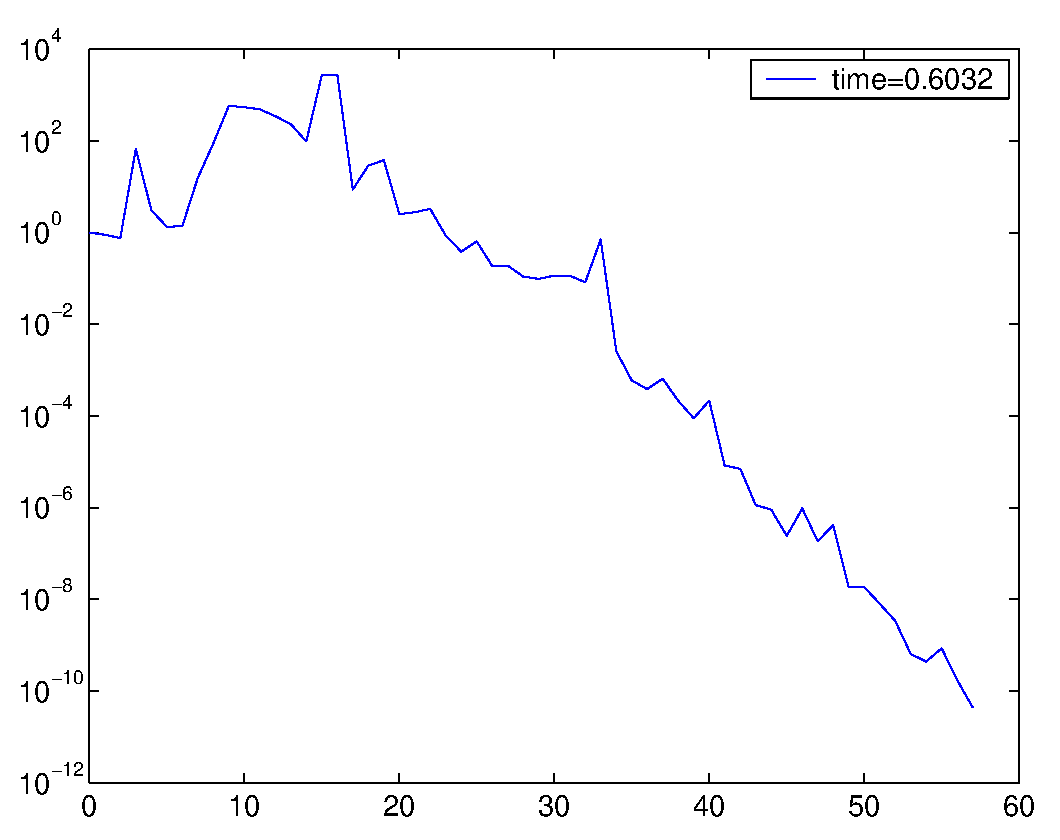
\includegraphics[scale=0.35]{eps/mp3bicgN20e50.eps}\hfill\includegraphics[scale=0.35]{eps/mp3bicgN20e1.eps}
\caption{Konvergenzgeschichte f"ur BiCG, Modellproblem III. Links:$N=20,
\epsilon = 50$, rechts $N=20, \epsilon = 1$}
\end{figure}


\begin{aufg}
Sei $A \neq A^H$, aber mit einer der folgenden speziellen Eigenschaften:
\begin{enumerate}
\item $A^H = \overline{A} \in \cnn$ (z.B. bei der Diskretisierung der Maxwell-Gleichungen in der Elektrodynamik)
\item $A^HJ = J^HA,\ J \in \cnn,\ J=J^H$ (man nennt $A$ dann auch {\em
$J$-hermitesch})
\item $A^TJ = J^TA,\ J \in \cnn$ (man nennt $A$ dann auch {\em $J$-symmetrisch})
\end{enumerate}
Zeige jeweils: F�r geeignete Wahl von $\tilde{r}^0$ (bzw. $w^0$) kann man den unsymmetrischen Lanczos-Prozess mit nur einer MVM mit $A$
(und eventuell einer zus�tzlichen mit $J$) durchf�hren
(dies �bertr�gt sich dann auch auf BiCG).
\end{aufg}
% Dieses Kapitel habe ich im Sommer 2007 neu geschrieben,
% weil mit dem Paper von Liessen, Faber und Tichy nun ein besserer
% Beweis fr den Faber-Manteuffel-Satz vorliegt
%
% Andreas Frommer, 22.6.2007


\newcommand{\kernel}{\mbox{Kern}}
\section{Minimales Residuum vs kurze Rekursion}

Das zentrale Resultat dieses Kapitels ist der Satz von Faber und Manteuffel,
Satz~\ref{faber:sa}. Zur Vorbereitung wiederholen wir ein paar 
Tatsachen "uber lineare Operatoren auf endlich-dimensionalen R"aumen, wie man sie aus
den Anf"angervorlesungen zur Linearen Algebra kennt. $A$ bezeichnet einen 
linearen Operator auf einem solchen Raum $V$ "uber $\MathC$, der mit einem Innenprodukt
$\langle \cdot, \cdot \rangle$ ausgestattet ist.

\begin{defn} 
 Die Adjungierte $A^*$ zu $A$ bez"uglich $\langle \cdot , \cdot \rangle$ ist die Matrix mit
\[
 \langle Ax , y  \rangle = \langle x, A^*y\rangle \quad \forall \; x,y \in V.
\]
\end{defn}

\begin{lem} \label{normal_eq:lem}
Die folgenden Bedingungen sind "aquivalent:
\begin{itemize}
 \item[(i)] $AA^* =  A^*A $,
 \item[(ii)] $V$ besitzt eine Orthonormalbasis aus Eigenvektoren $q_i$ von $A$ (zu Eigenwerten $\lambda_i$),
 \item[(iii)] $A^*=p(A), \quad p \in \Pi_{n-1}$, wobei $n = \dim(V)$.
\end{itemize}
\end{lem}
\begin{proof}
 (i) $\Leftrightarrow$ (ii) ist bekannt aus LA.

 (ii) $\Longrightarrow$ (iii): Aus $\langle q_j, A^*q_i \rangle = \langle Aq_j, q_i \rangle 
  = \lambda_j \delta_{ij}$ folgt $A^*q_i = \overline{\lambda}_i q_i$.
 Daraus folgt $A^* = p(A)$, wobei $p$ das Polynom aus
$\Pi_k$ ist mit $p(\lambda_i)=\overline{\lambda_i}, \quad i=1, \dots,k$. Dabei sind  $\lambda_1,\dots,\lambda_k$ die {\em verschiedenen}
Eigenwerte von $A$.

 (iii) $\Longrightarrow$ (i): trivial.
\end{proof}
%

\begin{defn} 
Ein linearer Operator, der eine der drei Bedingungen aus Lemma~\ref{normal_eq:lem}
erf"ullt, hei"st {\em normal}. $A$ hei"st {\em $s$-normal} ($s \in \mathbb{N}, s < \dim(V)$), falls 
$s$ der kleinste Grad von allen Polynomen ist, die 
Lemma~\ref{normal_eq:lem} (iii) erf"ullen.
\end{defn}
\medskip

Beispiel: $A$ selbstadjungiert $\Rightarrow$ $A$ ist 1-normal.
\medskip

\begin{aufg} Charakterisiere alle 1-normalen Operatoren.
\end{aufg}

\begin{defn}
$\mu_A$ und $d_A$ bezeichnen das Minimalpolynom von $A$ und dessen Grad. 
\\
F"ur $v \in V$ bezeichnen $\mu_v$ und $d_v$ das Minimalpolynom von $v$ bzgl.\ $A$
und dessen Grad. D.h., $\mu_v$ ist das Polynom kleinsten Grades mit 
$\mu_v(A)v = 0$, normiert auf H"ochstkoeffizient 1.
\end{defn}

\begin{lem} Gilt $p(A)v = 0$, so folgt $\mu_v \mid p$. Insbesondere
gilt $\mu_v \mid \mu_A$.
\end{lem}  
\begin{proof} Alle Polynome mit $p(A)v = 0$ bilden ein Ideal. Weil
der Polynomring ein Hauptidealring ist, liegen sie alle in dem 
von $\mu_v$ erzeugten Hauptideal.
\end{proof}

\begin{defn} Der von $v \in V$ erzeugte {\em zyklische Unterraum} ist
\[
   K(A,v) = K_{d_v}(A,v).
\]
Beachte: $d_v$ ist der Stufenindex, ab dem $K_m(A,v)$ stagniert.
\end{defn}

\begin{lem} \label{normal_tat1:lem}
Tatsachen "uber zyklische Unterr"aume:
\begin{itemize}
\item[(i)] $\hat{A}: K(A,v) \to K(A,v), \, w \to Aw$ ist linearer Operator auf $K(A,v)$.
\item[(ii)] F"ur $ w \in K(A,v)$ ist $K(A,w) \subseteq K(A,v)$. Gleichheit gilt genau dann,
          wenn $w = p(A)v$ mit $p$ ist teilerfremd zu $\mu_v$. 
\item[(iii)] Eigenr"aume in $K(A,v)$ haben immer Dimension 1.
\end{itemize}
\end{lem}
\begin{proof}
(i) ist klar; ebenso der erste Teil von (ii). F"ur $w = p(A)v$ gilt wegen $K(A,w) \subseteq 
K(A,v)$  einerseits $\mu_w \mid \mu_v$. Andererseits gilt
 $\mu_v \mid p \cdot \mu_w$. Dies beweist den Rest von (ii). Ein Eigenvektor $p(A)v$ zum Eigenwert $\lambda$
erf"ullt $(Ap(A)-\lambda p(A))v = 0$ mit $\deg p \leq d_v-1$. Also ist sogar $\mu_v = \alpha \cdot (t-\lambda) \cdot p(t)$,
was den Eigenvektor bis auf skalare Vielfache eindeutig festlegt.
\end{proof}

\begin{lem} \label{normal_tat2:lem}
Weitere Tatsachen:
\begin{itemize}
\item[(i)] Mit $\mu_A(t) = \prod_{i=1}^\ell (t-\lambda_i)^{e_i}$ gilt
\[
V = \oplus_{i=1}^\ell \kernel(A-\lambda_i I)^{e_i}
\]
\item[(ii)] Zu jedem $p \in \Pi$ mit $p \mid \mu_A$ existiert $u \in V$ mit $\mu_u = p$.
\end{itemize}
\end{lem}
\begin{proof} (i) ist bekannt. In (ii) nimmt man f"ur $p = \prod_{i=1}^\ell (t-\lambda_i)^{f_i}$ mit $f_i 
\leq e_i$ den Vektor $u = \sum_{f_i > 0} u_i$ mit $u_i \in \kernel(A-\lambda_i I)^{f_i} -
 \kernel(A-\lambda_i I)^{f_i-1}$.
\end{proof}
\medskip

Wir ben"otigen zwei technische Lemmas. 

\begin{lem} \label{FMproof1:lem}
$A,B: V \to V$ seien linear, $A$ invertierbar. Weiter sei $s+2 \leq d_A$ und 
f"ur alle $v \in V$ mit $d_v = d_A$  gelte
\[
Bv \in \spann(v,A,\ldots,A^s v).
\]
\begin{itemize}
\item[(i)] Dann gilt $AB = BA$.
\item[(ii)] Im Fall $B = A^*$ folgt: $A$ ist $t$-normal mit $t \leq s$.
\end{itemize} 
%Im Fall $B = A^*$ gilt sogar, dass dann $A$ $t$-normal ist
%mit $t \leq s$.
\end{lem}
\begin{proof}
(i): Sei $d_v = d_A$. F"ur $\gamma \not \in \spek(A)$ folgt mit $w_\gamma = (A-\gamma I)v$
aus Lemma~\ref{normal_tat1:lem}, dass $K(A,v) = K(A,w_\gamma)$ und $d_v = d_{w_\gamma}$; insbesondere gilt das f"ur $w_0 = Av$. Nach Voraussetzung existieren Polynome $p_\gamma,
q,r \in \Pi_s$ mit
\begin{equation} \label{BAs:eq}
   Bw_\gamma = p_\gamma(A)w, \; B(Av) = q(A)(Av), \; Bv = r(A)v,
\end{equation}
also
\[
Bw_\gamma = (p_\gamma(A)\cdot(A -\gamma I))v = B(Av)-\gamma Bv = (q(A)\cdot A - \gamma r(A))v. 
\]
F"ur $\gamma \not \in \spek(A)$ erf"ullt das Polynom $\phi_\gamma(t) = t\cdot(p_\gamma(t)-q(t))-\gamma(p_\gamma(t)-r(t)) \in \Pi_{s+1}$ 
also $\phi_\gamma(A)v = 0$, ist also Vielfaches von $\mu_v$. Wegen $\leq s+1 \leq d_v$
folgt $\phi_\gamma \equiv 0$. Hieraus folgt 
\[
   \gamma(q-r) = (t-\gamma)(p_\gamma - q),
\]
d.h.\ jedes $0 \neq \gamma \not \in \spek(A)$ ist Nullstelle von $q-r$,
also $q=r$ und damit nach \eqnref{BAs:eq} $BAv = q(A)Av = ABv = Ar(A)v$. 

Die Operatoren
$A$ und $B$  kommutieren also auf allen Vektoren $v$ mit $d_v = d_A$. F"ur einen gegebenen solchen Vektor
ist $\mbox{dist}(A^{d_v-1}v,\spann(v,\ldots,A^{d_v-2}v)) >0$; aus Stetigkeitsgr"unden 
gilt das dann auch noch, wenn man $v$ durch ein beliebiges $w$ aus einer gen"ugend kleinen 
Kugel um $v$ ersetzt. F"ur alle solche $w$ ist also $d_w = d_v$; insbesondere gibt
es eine Basis $b_1,\ldots,b_n$ von $V$ mit $d_{b_i} = d_v$. Gezeigt wurde bereits
$ABb_i = BAb_i$, also gilt $AB = BA$. \smallskip \\
(ii): Nach (i) ist $A$ normal, also $A^* = p(A)$ mit $\deg p \leq d_A-1$. F"ur ein $v$ mit 
$d_v = d_A$ gilt aber $A^*v = p(A)v \in \spann(v,Av,\ldots,A^sv)$. Weil $v,Av,\ldots,A^{d_A-1}v$
l.u.\ sind, folgt daraus $\deg p \leq s$.
\end{proof}
\medskip

Jetzt betrachten wir das Arnoldi-Verfahren \ref{Arnoldi-Verfahren} in
Abh"angigkeit vom Startvektor $v = h_{1,0}v_1 $. Zur Erinnerung: Man berechnet
eine ONB $\{v_1,v_2,\ldots\}$ durch
\begin{equation} \label{Arnoldi_rek.eq}
h_{i+1,i} v_{i+1} = Av_i - \sum_{j=1}^{i} h_{j,i}v_j.
\end{equation}
F"ur gegebenen Startvektor $u,v,w,x,\ldots$ bezeichnen dann $u_i,v_i,w_i,x_i, \ldots$
die entsprechenden Arnoldi-Vektoren. 

\begin{lem} \label{FMproof2:lem}
$A: V \to V$ sei linear und invertierbar. Es sei $1 < i \leq m < n \leq d_A$.
F"ur alle $u \in V$ mit $d_u = n$ gelte $\langle u, Au_i \rangle =0$. Dann gilt
auch f"ur alle $v$ mit $i \leq d_v \leq n$ die Beziehung $\langle v, Av_i \rangle = 0$.
\end{lem}
\begin{proof}
Sei $v \in V$ mit $i \leq  d_v < n$. Sei $u \in V$ mit $d_u = n$ so, dass $\mu_v \mid \mu_u$. 
(Erg"anze $\mu_v$ um $d_u-d_v$ Linearfaktoren aus Eigenwerten und verwende Lemma \ref{normal_tat2:lem}(ii).)  Setze
\[
x_\gamma = v - \gamma u.
\]
Klar: $\mu_{x_\gamma} \mid \mu_u$. Angenommen, $\mu_{x_\gamma}$ ist echter Teiler
von $\mu_u$. Dann gilt
\begin{equation} \label{mugamma:eq}
  \mu_{x_\gamma}(A)v = \gamma \underbrace{\mu_{x_\gamma}(A)u}_{\neq 0}.
\end{equation}
Es gibt nur endlich viele Teiler von $\mu_u$. F"ur jeden solchen Teiler $\mu_{x_\gamma}$
wird \eqnref{mugamma:eq} f"ur nur ein $\gamma$ erf"ullt. F"ur alle bis auf endlich viele
$\gamma$ ist also $\mu_{x_\gamma} = \mu_u$. Sei jetzt $x = x_\gamma$ f"ur ein $\gamma$,
das keine Ausnahme ist. Dann ist im Arnoldi-Verfahren $x_i = p(A)x$ mit $p \in \Pi_{i-1}$
und es gilt f"ur $j=0,\ldots,i-2$
\[
  0 = \langle A^j x, x_i \rangle = \langle A^j x, p(A)x \rangle
\]
und, nach Voraussetzung,
\[
\langle x , Ax_i \rangle  = \langle x, Ap(A)x \rangle = 0.
\]
Dies sind $i$ Gleichungen eines homogenen LGS f"ur die $i$ Koeffizienten 
von $p \neq 0$, d.h. die Determinante
\[
\delta(x) = 
\left| 
\begin{array}{cccc}
   \langle x, x \rangle & \langle x, Ax \rangle & \ldots & \langle x, A^{i-1} x \rangle \\
  \langle Ax, x \rangle & \langle Ax, Ax \rangle & \ldots & \langle Ax, A^{i-1} x \rangle \\
    \vdots              &    \vdots              &    \ldots & \vdots \\
 \langle A^{i-2}x, x \rangle & \langle A^{i-2}x, Ax \rangle & \ldots & \langle A^{i-2}x, A^{i-1} x \rangle \\
 \langle x, Ax \rangle & \langle x, A^2x \rangle & \ldots & \langle x, A^{i} x \rangle 
\end{array}
              \right|
\]
verschwindet f"ur $x = x_\gamma$ f"ur alle bis auf endlich viele und damit f"ur alle
$\gamma$. Also existiert auch f"ur $\gamma = 0$, also $x=v$ eine nicht-triviale L"osung
des zugeh"origen LGS in Gestalt eines Polynoms $0 \neq q \in \Pi_{i-1}$. Die ersten
$i-1$ Gleichungen besagen, dass $0 \neq w = q(A)v$ orthogonal zu
$\spann(v,Av,\ldots,A^{i-2} v)$,
also Vielfaches von $v_{i}$ ist. Die letzte Gleichung besagt $\langle v, Aw \rangle = 0$,
also $\langle v, Av_i \rangle = 0$. 
\end{proof}


\begin{defn} $A$ {\em erlaubt eine $s$-stellige Rekursion}, wenn im
Arnoldi-Verfahren f"ur jeden Startvektor $v$ gilt $h_{j,i} = 0$ f"ur
$j < i-s$ und es einen Startvektor gibt, f"ur den f"ur wenigstens
ein $i$ die Zahl $h_{i-s,i} \neq 0$. 
\end{defn}


\begin{sa}[Faber, Manteuffel 1982] 
\label{faber:sa}
$A$ erlaubt eine $s$-stellige Rekursion mit $s+2 \leq d_A$
 $\Longleftrightarrow$ $A$ ist $s$-normal. 
\end{sa}
\begin{proof}
"`$\Leftarrow$"': Es ist $h_{i,j} = \langle Av_i,v_j \rangle = \langle v_i, A^*v_j \rangle$
mit $A^* = p(A), p \in \Pi_s$. Also
\[
\langle v_i, \underbrace{p(A)v_j}_{\in K_{j+s}} \rangle = 0 \mbox{ f"ur } j+s \leq i-1.
\]
"`$\Rightarrow$"' (der harte Teil!): \\
{\em Teil I: Einschr"ankung auf $K(A,v)$ mit $d_v = s+2$.}\\
Nach Voraussetzung gilt
\begin{equation} \label{FMproof:eq}
\langle v, Av_{s+2} \rangle = 0 \enspace \mbox{f"ur alle } v \in V \mbox{ mit } d_v = s+3.
\end{equation}
Sei $u \in V$ mit $d_u = s+2$. Sei $\hat{A}: K(A,u) \to K(A,u), \, u \to Au$. Es
ist $d_u = d_{\hat{A}} = \dim K(A,u)$. Sei $y \in K(A,u)$ mit $d_y = d_u$
(bzgl.\ $A$ wie $\hat{A}$). Wegen \eqnref{FMproof:eq} und Lemma~\ref{FMproof2:lem}
gilt
\[
0 = \langle y, Ay_{s+2} \rangle =  \langle y, \hat{A}y_{s+2} \rangle = 
\langle \hat{A}^*y, y_{s+2} \rangle .
\]
Also gilt $\hat{A}^*y \in \spann(y,\hat{A}y,\ldots,\hat{A}^s y)$. Nach Lemma~\ref{FMproof1:lem}(ii)
folgt: $\hat{A}$ ist $t$-normal mit $t \leq s = \dim K(A,u) -1$. Insbesondere gilt mit paarweise
verschiedenen $\lambda_i$
\[
  K(\hat{A},y) = \kernel(\hat{A}-\lambda_1 I) \oplus_\perp \kernel(\hat{A}-\lambda_2 I) \oplus_\perp 
         \ldots \oplus_\perp \kernel(\hat{A}-\lambda_{s+2} I).
\]
(Alle Eigenr"aume sind 1-dimensional nach Lemma~\ref{normal_tat1:lem}(iii).).
\smallskip

{\em Teil II: "Ubertragung auf ganz $V$.} \\
Sei $v \in V$ mit $d_v = d_A$. Dann ist
\[
K(A,v) = \oplus_{i=1}^\ell K(A,z_i) \mbox{ mit } \mu_{z_i}(t) = (t-\lambda_i)^{c_i}.
\]
Wieder sind die $\lambda_i$ paarweise verschieden. OBdA seien sie nach absteigenden
$c_i$ nummeriert. Wegen $\dim(K(A,w)) = d_A > s+2$ existiert $m \leq \ell$ und $\tilde{c}_m
\leq c_m$ mit $c_1+\ldots + c_{m-1} + \tilde{c}_m = s+2$. Der Vektor $w = z_1 + \ldots +z_{m-1}
+ z_{m-1} + \tilde{z}_m$ mit $\tilde{z}_m \in \kernel(A-\lambda_m I)^{\tilde{c}_m} - 
\kernel(A-\lambda_m I)^{\tilde{c}_m-1} $ hat $d_w = s+2$. Nach Teil~I besitzt $A$ 
demnach $s+2$
verschiedene Eigenwerte auf $K(A,w)$, weshalb $c_1 = \ldots = \tilde{c}_m=1$ und damit
sogar $m=\ell$ und $c_1 = \ldots = c_\ell = 1$. Damit ist
\[
\mu_A(t) = \mu_w(t)  = \prod_{i=1}^\ell (t-\lambda_i)^1
\]
und deshalb (LA I)
\[
V = \oplus_{i=1}^\ell \kernel (A - \lambda_i I).
\]
Setze $V_i = \spann(z_i,\ldots,z_{s+i+1}) = K(A,\sum_{j=i}^{s+i+1} z_j)$
mit $z_j \in \kernel(A-\lambda_j I)$. Nach Teil I ist
\[
V_i = \kernel(A-\lambda_i I) \oplus_\perp \kernel(A-\lambda_{i+1} I) \oplus_\perp 
         \ldots \oplus_\perp \kernel(A-\lambda_{s+i+1} I),
\]
und es existiert ein Polynom $p_i \in \Pi_{s}$ mit $p_i(\lambda_j) = \overline{\lambda_j},
\, j=i,\ldots,s+i+1$. Die Polynome $p_i$ und $p_{i+1} \in \Pi_s$ stimmen in den $s+1$ Stellen $\lambda_{i+1}, \ldots, \lambda_{s+i+1}$ "uberein, sind also (alle!) identisch, $p_1=p_2
= \ldots p_\ell = p$.
\\
Zusammengefasst: $A$ ist orthogonal diagonalisierbar und es existiert $p \in \Pi_s$ mit $p(\lambda) = 
\overline{\lambda}$ f"ur alle $\lambda \in \spek(A)$. Also ist $A$ $s$-normal.
\end{proof}
\medskip

Frage: Haben wir auch gezeigt, dass $s$ nicht kleiner sein kann?
\medskip

Im Falle des Standard-Innenproduktes und der Standardbasis 
besitzt $A^*$ als Matrix die Darstellung
\[
A^* = \overline{A}^T.
\]

Wie ist dies bei einem beliebigen Innenprodukt (der Satz legt sich ja
nicht fest)? \\
Wechsel in der Notation: $\langle \; , \; \rangle_*$ ist jetzt ein beliebiges
Innenprodukt, $\langle \; , \; \rangle$ das "ubliche euklidische Innnenprodukt.

%
\begin{lem}
 Sei $\langle \; , \; \rangle_*$ ein Innenprodukt auf  $\cn$.
 Dann existiert ein $B \in \cnn$, $B$ hpd mit
\[\langle x , y \rangle_* = \langle x,B y \rangle \enspace (\mbox{$\langle \; , \; \rangle$ "ubliches Skalarprodukt).} \]
\end{lem}
\begin{proof}
 "Ubung.
\end{proof}
%
\begin{sa}
 Sei $\langle \; , \; \rangle_*$ gegeben und $B$ hpd mit $\langle x, y \rangle_*$ = $\langle y, By\rangle$. Dann gilt:  $A$ ist normal bzgl.
$\langle \; , \; \rangle_* \Longleftrightarrow B^{\frac{1}{2}}AB^{-\frac{1}{2}} $ ist normal bzgl. $\langle \; , \; \rangle$.
\end{sa}
\begin{proof}
 \begin{align*}
  && \langle Ax, y\rangle_*  & = \langle x, A^*y\rangle_* \\
  & \Longleftrightarrow &  \langle Ax, By\rangle & =  \langle x, BA^*y\rangle \\
  & \Longleftrightarrow &  \langle BAx, y\rangle & =  \langle x, BA^*y\rangle \quad \forall \; x,y \\
  & \Longleftrightarrow  & (BA^*)^H   & =  BA   \\
  & \Longleftrightarrow  & BA^* & =  A^HB  \\
  & \Longleftrightarrow & A^* & = B^{-1}A^HB.
 \end{align*}
Es ist also
 \begin{align*}
  && A^*A & =AA^* \\
  & \Longleftrightarrow & B^{-1}A^HBA  & = AB^{-1} A^HB  \\
  & \Longleftrightarrow  & B^{-\frac{1}{2}}A^H B^{\frac{1}{2}}B^{\frac{1}{2}}AB^{-\frac{1}{2}}  & = B^{\frac{1}{2}}AB^{-\frac{1}{2}}B^{-\frac{1}{2}}A^HB^{\frac{1}{2}}   \\
  & \Longleftrightarrow  & \tilde{A}^H \tilde{A}  & = \tilde{A} \tilde{A}^H
 \end{align*}
mit $\tilde{A}=B^{\frac{1}{2}}AB^{-\frac{1}{2}}$.
\end{proof}
%

\medskip

\textbf{Bezeichnung:} Statt "`$A$ normal bzgl. $\langle \; , \; \rangle_*$"' sagt man auch: "`$A$ ist $B$-normal"' ($B$ ist die zu
$\langle \; , \; \rangle_*$ geh"orige hpd-Matrix).
%
\begin{cor}
 $A$ ist $B$-normal $\Longleftrightarrow \exists \; p \in \Pi_n$ mit $A^*=p(A)$.
\end{cor}
\begin{proof}
 \begin{align*}
 A \text{ ist $B$-normal} & \Longrightarrow    & \tilde{A}    &= B^{\frac{1}{2}}AB^{-\frac{1}{2}} \text{ normal} \\
 & \Longrightarrow        & \tilde{A}^H     &= p(\tilde{A}) = B^{\frac{1}{2}}p(A)B^{-\frac{1}{2}} \\
 & \Longrightarrow        & B^{\frac{1}{2}}\tilde{A}^HB^{-\frac{1}{2}} &=p(A) \\
 & \Longrightarrow        & A^*        & = p(A)
 \end{align*}
\end{proof}
%

%% Vorlesung 18
%% Freitag, 27.6.2003
%% David Fritzsche

\textbf{Beachte:} Satz~\ref{faber:sa} setzt eine bestimmte Form f\"ur kurze
Rekursion voraus.

Alternative: z.B.~gekoppelte kurze Rekursion. Dann k\"onnten doch weitere
Verfahren mit minimalem Residuum und kurzer Rekursion existieren.

\begin{bsp}
  Sei $A\in\cnn$ unit\"ar, also $AA^H=I$. Es exisitiert eine kurze Rekursion
  zur Berechnung der Arnoldi-Vektoren
  \begin{equation*}
    h_{k,k+1}v^{k+1} = Av^k-\sum_{j=1}^{k}h_{k,j}v^j
    \qquad
    \text{mit }
    \norm{v^k}_2=1
    \text{ und }
    v^0=\frac{1}{\norm{r^0}}r^0.
  \end{equation*}
Die Vektoren
  $v^0,\dots,v^k$ sind eine Orthonormalbasis von $K_{k+1}(A,r^0)$ und
  {$Av^0,\dots,Av^k$} ist Orthonormalbasis von $AK_{k+1}(A,r^0)$.

  Damit ist $w^k,Av^0,\dots,Av^{k-1}$ bei geeigneter Wahl von $w^k$ eine
  Orthonormalbasis von $K_{k+1}(A,r^0)$.
  Eine geeignete Wahl ergibt sich induktiv "uber
  \begin{align*}
    \tilde w^k
    &= w^{k-1} - \sum_{j=0}^{k-1}
    \frac {\langle w^{k-1},Av^j\rangle} {\langle Av^j,Av^j\rangle} Av^j
    && (\langle Av^j,Av^j\rangle = 1)
    \\
    &= w^{k-1} - \sum_{j=0}^{k-1} \langle w^{k-1},Av^j\rangle Av^j
    && (w^{k-1}\perp Av^j \text{ f\"ur } j=0,\dots,k-2)
    \\
    &= w^{k-1} - \langle w^{k-1},Av^{k-1}\rangle Av^{k-1}
    &&
    \\
    w^k
    &= \frac{1}{\norm{\tilde w^k}}\tilde w^k
    .
    &&
  \end{align*}

  Die Berechnung von $v^{k+1}$ geht jetzt so:
  \begin{equation*}
    \tilde v^{k+1} = Av^k -\Bigl(\sum_{j=1}^{k}\beta_{k,j}Av^{j-1}\Bigr)
    - \beta_{k,0}w^k
  \end{equation*}
  \begin{align*}
    \text{mit}\qquad
    \beta_{k,j}
    &= \langle Av^k, Av^{j-1}\rangle = 0
    &&\text{da } v^k\perp v^{j-1}
    \\
    \beta_{k,0}
    &=
    \langle Av^k, w^k\rangle
    &&
  \end{align*}
  Wir erhalten also folgenden Algorithmus~\ref{alg:unitaeres-arnoldi-verf}
  zur Berechnung der Arnoldi-Vektoren.

  \begin{alg}[Unit\"ares Arnoldi-Verfahren]\label{alg:unitaeres-arnoldi-verf}
    \begin{algorithm}
      \begin{algorithmic}
        \STATE $v^0 := \bigl(1/\norm[normal]{r^0}\bigr)r^0$
        \STATE $w^0 := v^0$
        \FOR{$k=0,1,2,\dots$}
          \STATE $\beta_k = \langle Av^k,w^k\rangle$
          \STATE $\tilde v^{k+1} := Av^k-\beta_k w^k$
          \STATE $v^{k+1}
            :=\bigl(1/\norm[normal]{\tilde v^{k+1}}\bigr)\tilde v^{k+1}$
          \STATE $\tilde w^{k+1} := w^k-\overline{\beta}_k Av^k$
          \STATE $w^{k+1}
            :=\bigl(1/\norm[normal]{\tilde w^{k+1}}\bigr)\tilde w^{k+1}$
        \ENDFOR
      \end{algorithmic}
    \end{algorithm}
  \end{alg}

  Jetzt ist $H_{k,k}$ und $H_{k+1,k}$ aus dem Arnoldi-Prozess nicht
  mehr explizit gegeben. Man kann aber zeigen (Jagels und Reichel, 1994)
  \begin{enumerate}
  \item $H_{k,k}$ wird durch Algorithmus~\ref{alg:unitaeres-arnoldi-verf}
    in faktorisierter Form (als Produkt von Rotationen) implizit gegeben.
  \item F\"ur Systeme der Form
    \begin{equation*}
      (\zeta I+\rho A)x=b
    \end{equation*}
    mit $A^HA=I$ und $\zeta,\rho\in\co$ ist
    $K_m(\zeta I+\rho A,r^0)=K_m(A,r^0)$ und es existiert auch eine
    kurze Rekursion zur Bestimmung der Iterierten $x^k$ mit
    \begin{equation*}
      \norm[big]{b-(\zeta I+\rho A)x^k}_2
      =
      \min_{p_k\in\bar \Pi_k}
      \norm[big]{p_k(\zeta I+\rho A)b}_2
      .
    \end{equation*}
    Die Herleitung erfolgt wie bei MINRES unter Ausnutzung der faktorisierten
    Form von $H_{k+1,k}$
  \end{enumerate}

\end{bsp}




%%% Local Variables:
%%% mode: latex
%%% TeX-master: "Iterationsverfahren03"
%%% End:


\include{kap12}
\section[Modellproblem IV]{Modellproblem IV: Overlap-Fermionen in der Gittereichtheorie}

Die Gittereichtheorie befasst sich mit der Diskretisierung der
Quantenchromodynamik (QCD). QCD ist die Theorie der starken
Wechselwirkung zwischen den Quarks.

\begin{defn}
  Die \emph{Wilson-Fermi-Matrix} $M$ beschreibt eine
  N\"achste-Nachbar-Kopplung auf einem \"aquidistanten
  $4$-dimensionalen Gitter
  \begin{equation*}
    G=\bigl\{ x\in\{1,\dots,N\}^4\bigr\}
    \qquad
    e_1=(1,0,0,0),\ e_2=(0,1,0,0),\ \dots
  \end{equation*}
  durch
  \begin{equation}
    \label{eq:wilson-fermi-matrix}
    \begin{aligned}
      (M\psi)_x
      =
      \psi_x-\kappa\biggl(
      & \sum_{\mu=1}^{4}
      \bigl(U_{x}^\mu\otimes (I-\gamma_\mu)\bigr)
      \psi_{x-e_\mu}
      \\
      +
      & \sum_{\mu=^1}^{4}
      \bigl(U_{x+e_\mu}^\mu\otimes(I+\gamma_\mu)\bigr)
      \psi_{x+e_\mu}
      \biggr)
    \end{aligned}
  \end{equation}
  mit $\psi_x\in\co^{12}$ (12 Unbekannte pro Gitterpunkt),
  $\gamma_\mu\in\co^{4\times 4}$,
  $U_x^\mu\in\mathord{\mathrm{SU}}(3)$ (unit\"are Matrizen mit Determinante +1).
   Dabei ist $\kappa\in(0,4)$ anpassbar und $U_x^\mu$
  zuf\"allig erzeugt. Gleichung \eqref{eq:wilson-fermi-matrix} ist an den
  R\"andern von $G$ periodisch zu verstehen.

  Es ist also $M\in\cnn$ mit $n=12\cdot N^4$.
  Heutzutage (Sommer 2024) liegt $N$ zwischen $32$ und $256$.
  \begin{center}
    \begin{tabular}{|r|l@{ }r|}\hline
      $N$   & \multicolumn{2}{c|}{$n$} \\ \hline
      $32$  & ca. & $1.2\cdot 10^7$ \\
      $64$  & ca. & $  2\cdot 10^8$ \\
      $128$ & ca. & $  3\cdot 10^9$ \\ \hline
    \end{tabular}
  \end{center}
\end{defn}


Beim sog.\ {\em Overlap-Fermionen-Modell} muss man
Systeme der Gestalt
\begin{equation}
  \label{eq:overlap-fermionen}
  \bigl(I+m\,\Gamma_{\!5} \sgn(Q)\bigr)\psi = \phi
\end{equation}
l�sen mit
\[
\Gamma_5 = I_{\frac{n}{4}} \otimes \gamma_5, \enspace \gamma_5 = \diag(1,1,-1-1),
\]
$Q=\Gamma_{\!5}M$ hermitesch, $Q=V\Lambda V^H$ und $m\lesssim 1$.

Dabei ist $\sgn(Q)$ definiert als $\sgn(Q)=V\sgn(\Lambda)V^H$ mit
\[
	\sgn(\Lambda)=\diag(\sgn(\lambda_i))
\]
f\"ur $\Lambda=\diag(\lambda_i)$.

\begin{bem}
  \begin{enumerate}
  \item Es gilt $\Gamma_{\!5}=\Gamma_{\!5}^H=\Gamma_{\!5}^{-1}$
    (siehe Physik) und $\sgn(Q)\cdot\sgn(Q)=I$ (falls $Q$ regul\"ar)
    mit $\sgn(Q)=(\sgn(Q))^H$. Also sind $\Gamma_{\!5}$ und
    $\sgn(Q)$ unit\"ar, also auch $\Gamma_{\!5}\cdot\sgn(Q)$.
    Auf \eqref{eq:overlap-fermionen} kann also das Verfahren vom Ende
    des letzten Abschnittes angewendet werden.
  \item $\sgn(Q)$ kann man praktisch nicht explizit berechnen. Der
    Aufwand w"are $O(n^3)$ f\"ur die Zeit und $O(n^2)$ f\"ur den
    Speicher.  F\"ur ein KUV   zur L"osung von \eqnref{eq:overlap-fermionen}
    gen\"ugt es aber, wenn man in jedem
    Schritt $\sgn(Q)y$ berechnen kann.
  \end{enumerate}
\end{bem}


$\sgn(Q)y$ kann man mit Hilfe des Lanczos-Verfahrens berechnen:

Es ist
\begin{align*}
  \sgn(Q)  &= (Q^2)^{-1/2}Q \\
  \sgn(Q)y &= (Q^2)^{-1/2}Qy .
\end{align*}
Sei $V_m=(v^1|\dots|v^m)$ die Matrix mit den Lanczos-Vektoren f\"ur $Q^2$
mit Start $v^1=Qy$ und $\norm{Qy}=1$. Dann gilt
\begin{equation*}
  Q^2V_m = V_{m+1}T_{m+1,m}.
\end{equation*}
Daraus folgt $V_m^HQ^2V_m = T_{m,m}$ (tridiagonal).

\smallskip

\textbf{Idee:} Approximiere
\begin{align*}
  \sgn(Q)y
  &= (Q^2)^{-1/2}Qy
  \\
  &\approx V_m(T_{m,m}^{-1/2})\underbrace{V_m^HQy}_{=e^1}
\end{align*}
Dabei kann man $T_{m,m}^{-1/2}$ f\"ur moderates $m$ explizit durch
Berechnung der vollst\"andigen Basis aus Eigenvektoren bestimmt werden.

\begin{sa}
  Es gilt
  \begin{equation*}
    \norm{\sgn(Q)y-V_m(T_{m,m}^{-1/2})V_m^HQy}_2
    \leq
    \norm{r^m}_2
  \end{equation*}
  mit $r^m={}$Residuum von CG f\"ur $Q^2x=y$, Startwert $x^0=0$.
\end{sa}

\begin{proof}
  Man verwendet
  \begin{enumerate}
  \item
    \begin{align*}
      a^{-1/2}
      &=
      \frac{2}{\pi}\int_0^{\infty}(a+t^2)^{-1}\;dt
      \\
      \Longrightarrow\;(Q^2)^{-1/2}
      &=
      \frac{2}{\pi}\int_0^\infty (Q^2+t^2I)^{-1}\;dt
    \end{align*}
  \item Ist $r_t^m$ das Residuum von CG f\"ur $(Q^2+t^2I)x=y$, so gilt
    $\norm{r_t^m}_2\leq\norm{r_0^m}_2$.\\
    Es gilt sogar: $r_t^m=\psi_{t,m}r_0^m$ mit $\abs{\psi_{t,m}}<1$.
  \end{enumerate}

  Der Beweis wird nur skizziert.
Wir leiten zuerst die Absch�tzung f�r die Residuen her:
$$r_i^k=p_{i,k}(Q^2+ t^2 I)b \perp K_k(Q^2). $$
Damit gibt es also ein Polynom $p_{k,0}$ mit
$$p_{k,i}(Q^2+t^2 I)b = \Phi_{k,t} p_{k,0}(Q^2)b .$$
Wenn man das Polynom nun in $t$ betrachtet ergibt dies
\begin{align*}
p_{k,t} ( s + t^2) &= \Phi_{k,t} p_k(s) \\
p_{k,t} ( s ) &= \Phi_{k,t} p_k(s-t^2)\\
\end{align*}
und da $p_{k,t}(0) = 1$, ist $\Phi_{k,t} = (p_k(-t^2))^{-1}$. Die Nullstellen der
Polynome sind die Ritz-Werte und daher $>0$.  Wegen $p(0) =1$ folgt so $p(s) > 1 $
f�r $s < 0$ und damit $|\Phi_{k,t}| < 1$. \medskip

Nun ist noch die Absch�tzung zu beweisen. Dazu betrachtet man
\begin{eqnarray*}
\lefteqn{\sgn(Q)b - Q V_m T_m^{-\frac 12} V_m^H b} \\
  &=& \frac{2}{\pi} \int_0^{\infty} Q(Q^2 + t^2I)^{-1}b - Q V_m(t^2I+T_m)^{-1}V_m^H b \; dt\\
  &=& \frac{2}{\pi} \int_0^{\infty} Q(Q^2 + t^2I)^{-1} \underbrace{\left[ b - (Q^2+t^2I) V_m(t^2I+T_m)^{-1}V_m^Hb\right]}_{= \psi_{t,m}r^m} \; dt.
\end{eqnarray*}
Weiter folgt wegen $| \psi_{t,m} \leq 1|$, dass alle Eigenwerte der hermiteschen Matrix
$$
\frac{2}{\pi} \int_0^{\infty} \psi_{t,m} Q(Q^2 + t^2I)^{-1} \, dt
$$
den Betrag $\leq 1$ haben. Damit ist auch die 2-Norm $\leq 1$.
\end{proof}



%%% Local Variables:
%%% mode: latex
%%% TeX-master: "Iterationsverfahren03"
%%% End:

 
\section{Pr"akonditionierung}

Gegeben wie immer:
\[
Ax = b
\]
Ziel: Beschleunigung der Konvergenz eines (passenden) KUV durch Modifikation der Matrix.

\begin{defn} Seien $M_L$ und $M_R$ invertierbar.
Dann bedeutet
\begin{itemize}
\item {\em rechtsseitige Pr"akonditionierung} den "Ubergang zu $AM_R^{-1}y = b$ (mit $x = M_R^{-1}$)
\item {\em linksseitige Pr"akonditionierung} den "Ubergang zu $M_L^{-1}Ax = M_L^{-1}b$ (mit neuer rechter Seite  $M_L^{-1}b$)
\item {\em beidseitige Pr"akonditionierung} den "Ubergang zu $M_L^{-1}AM_R^{-1}y = M_L^{-1}b$ (mit $x = M_R^{-1}$ und neuer rechter Seite  $M_L^{-1}b$)
\end{itemize}
\end{defn}

Das KUV wird dann mit der modifizierten Matrix (und evtl.\ rechten Seite) durchgef"uhrt.

\textbf{Anforderungen:}
\begin{enumerate}
   \item Die modifizierte Matrix sollte ``besser konditioniert'' sein, am besten $\approx I$
   \item $M_L^{-1}$ und $M_R^{-1}$ sind entweder einfach als d"unn besetzte Matrizen direkt gegeben, oder Systeme mit $M_L, M_R$ sind sehr effizient l"osbar (man muss sie in jedem Iterationsschritt l"osen).
\end{enumerate}

\begin{bsp}  Sei $A = D-L-U$ mit dem Diagonalteil $D$, unterem bzw. oberen Dreiecksanteil $-L$ bzw. $-U$.
\begin {itemize}
   \item Diagonaler Pr"akonditionierer: $M = D$, der Diagonalanteil von $A$. $M^{-1}$ ist sehr einfach zu invertieren.
   \item Unteres Dreieck als Pr"akonditionierer: $M = D-L$. Systeme mit $M$ sind leicht zu l"osen.
\end{itemize}
\end{bsp}



\subsection{Pr"akonditionierung von CG}
$A$ hpd. Notation: $M_L^{-1} =:S, M_R^{-1} = S^H$

\begin{eqnarray}\label{G451}
\begin{array}{rcl}
\wA \wx & = & \wb \hspace{1.2cm} \mbox{ mit } \\
\wA & = & S A S^H \, , S \mbox{ regul"ar } ( \Rightarrow \wA \mbox{ hpd}) \\
\wx & = & S^{-H} x \\
\wb & = & S b \, ,
\end{array}
\end{eqnarray}
wobei $ \mbox{cond}(\wA) \ll \mbox{cond}(A) $ sein soll.



Das CG-Verfahren f"ur \eqref{G451} lautet \smallskip


\noindent\textbf{Gegeben:} $ \wx_0, \;  \whr_0 = \wb - \wA \wx_0, \; \whp_0 = \whr_0, \;
\wq_0 = \wA \whp_0 $

\medskip

\noindent f"ur $ k = 0, 1, \ldots, m_0 -1 $
\begin{eqnarray}\label{G452}
\wx_{k+1} &=& \wx_k + \widehat{\alpha}_k \whp_k \mbox{ mit }
\widehat{\alpha}_k = \frac{\| \whr_k \|_2^2}{\langle \wq_k, \whp_k \rangle}\\
\whr_{k+1} & = & \whr_k - \widehat{\alpha}_k \wq_k \label{G453}\\
\whp_{k+1} & = & \whr_{k+1} + \widehat{\beta}_k\widehat{p}_k \label{G454}
\mbox{ mit } \widehat{\beta}_k = \frac{\| \whr_{k+1} \|_2^2}{\| \whr_k \|_2^2} \\
\wq_{k+1} & = & \wA \whp_{k+1} \label{G455}
\end{eqnarray}

\noindent R"ucktransformation in das urspr"ungliche System:

\begin{eqnarray*}
\wx_k & = &S^{-T} x_k \iff x_k = S^H \wx_k \\
\Rightarrow \underbrace{b - A x_k}_{=: r_k} & = & S^{-1}
\underbrace{(S b - S A S^H S^{-T} x_k)}_{\wb - \wA \wx_k}\; = \; S^{-1} \whr_k
\end{eqnarray*}

\noindent Multipliziere also \eqref{G452}, \eqref{G454} mit $ S^H$, \eqref{G453},
\eqref{G455} mit $ S^{-1}$ und setze
\begin{equation}
\left\{ \quad  \begin{array}{ll}
x_k &= S^H \wx_k, \\ r_k&= S^{-1} \whr_k \, ( = b - A x_k), \\ p_k &= S^H \whp_k, \\ q_k &= S^{-1} \wq_k .
\end{array}\right.\label{transf_eq}
\end{equation}
\medskip

Mit Hilfe von \eqref{transf_eq} formulieren wir die die Gleichungen \eqref{G452} bis \eqref{G455} um:
\begin{eqnarray*}
\widehat{\alpha}_k&=&\dfrac{\langle\widehat r_k,\widehat r_k\rangle }{\langle\widehat q_k,\widehat p_k\rangle }\\
&=&\dfrac{\langle Sr_k,Sr_k\rangle }{\langle Sq_k,S^{-T}p_k\rangle }\\
&=&\dfrac{\langle r_k,S^{T}Sr_k\rangle }{\langle q_k,S^HS^{-T}p_k\rangle }\\
&=&\dfrac{\langle r_k,M^{-1}r_k \rangle}{\langle q_k,p_k \rangle }\\
&=&\dfrac{\langle r_k,\widetilde{r}_k\rangle }{\langle q_k,p_k\rangle }\\
\widehat{\beta}_k&=&
\frac{\| \whr_{k+1} \|_2^2}{\| \whr_k \|_2^2}\\
&=&\dfrac{\langle Sr_{k+1},Sr_{k+1}\rangle }{\langle Sr_k,Sr_k\rangle }\\
&=&\dfrac{\langle r_{k+1},S^HSr_{k+1}\rangle }{\langle r_k,S^HSr_k\rangle }\\
&=&\dfrac{\langle r_{k+1},M^{-1}r_{k+1}\rangle }{\langle r_k,M^{-1}r_k\rangle }\\
&=&\dfrac{\langle r_{k+1},\widetilde{r}_{k+1}\rangle }{\langle r_k,\widetilde{r}_k\rangle }.
\end{eqnarray*}
Damit ergibt sich dann
\setcounter{equation}{1}
\renewcommand{\theequation}{\thesection.\arabic{equation}'}
\begin{eqnarray}
\notag\wx_{k+1} &=& \wx_k + \widehat{\alpha}_k \whp_k\\
\notag S^{-T}x_{k+1}&=&S^{-T}x_k +\dfrac{\langle r_k,\widetilde{r}_k\rangle }{\langle q_k,p_k\rangle }  S^{-T}p_k\\
x_{k+1}&=&x_k +\dfrac{\langle r_k,\widetilde{r}_k\rangle }{\langle q_k,p_k\rangle } p_k\\\notag\\
\notag \whr_{k+1} & = & \whr_k - \widehat{\alpha}_k \wq_k \\
\notag Sr_{k+1}&=&Sr_{k}-\dfrac{\langle r_k,\widetilde{r}_k\rangle }{\langle q_k,p_k\rangle }  Sq_k\\
r_{k+1}&=&r_{k}-\dfrac{\langle r_k,\widetilde{r}_k\rangle }{\langle Sq_k,S^{-T}p\rangle }  q_k\\\notag\\
\notag \whp_{k+1} & = & \whr_{k+1} + \widehat{\beta}_k\widehat{p}_k \\
\notag S^{-T}p_{k+1} & = & S r_{k+1}+\dfrac{\langle r_{k+1},\widetilde{r}_{k+1}\rangle }{\langle r_k,\widetilde{r}_k\rangle }S^{-T} {p}_k \\
\notag p_{k+1} & = & S^{T}S r_{k+1}+\dfrac{\langle r_{k+1},\widetilde{r}_{k+1}\rangle }{\langle r_k,\widetilde{r}_k\rangle } {p}_k \\
 p_{k+1}& = & \widetilde{r}_{k+1}+\dfrac{\langle r_{k+1},\widetilde{r}_{k+1}\rangle }{\langle r_k,\widetilde{r}_k\rangle } {p}_k \\\notag\\
\notag \wq_{k+1} & = & \wA \whp_{k+1} \\
\notag Sq_{k+1}&=&(SAS^H)(S^{-T}p_{k+1})\\
q_{k+1}&=&A p_{k+1}.
\end{eqnarray}
\renewcommand{\theequation}{\thesection.\arabic{equation}}

Dies liefert folgenden Algorithmus
\begin{alg}[Pr"akonditioniertes CG-Verfahren]\label{alg:pcg}
~\vspace*{-2\baselineskip}
\begin{algorithm}
%\caption{Pr"akonditioniertes CG-Verfahren}\index{CG-Verfahren!präkoditionites}\index{präkonditioniertes CG-Verfahren}
\begin{algorithmic}
\STATE w"ahle $x^{(0)}$ setze $r^{(0)}=b-Ax^{(0)}, p^{(0)}=r^{(0)}$, l"ose $M\hat r^{(0)}=r^{(0)}$
\FOR{$k=0,1,...,m_0-1$}
\STATE $x_{k+1}=x_k +\dfrac{\langle r_k,\widetilde{r}_k\rangle }{\langle q_k,p_k\rangle } p_k$
\STATE $r_{k+1}=r_{k}-\dfrac{\langle r_k,\widetilde{r}_k\rangle }{\langle q_k,p_k\rangle }  q_k$
\STATE l"ose $M\widetilde{r}_{k+1}={r}_{k+1}$
\STATE $p_{k+1} =  \widetilde{r}_{k+1}+\dfrac{\langle r_{k+1},\widetilde{r}_{k+1}\rangle }{\langle r_k,\widetilde{r}_k\rangle } {p}_k $
\STATE $q_{k+1}=A p_{k+1}$
\ENDFOR
\end{algorithmic}
\end{algorithm}
\end{alg}

\begin{aufg} Leite Algorithmus \ref{alg:pcg} alternativ dadurch her, dass CG mit dem $M$-Innenprodukt auf die im $M$-Innenprodukt selbstadjungierte und positiv definite Matrix $M^{-1}A$ angewendet wird.
\end{aufg}

$A$ hpd $\Rightarrow$ Diagonalanteil $D$ ist hpd. Diagonale Pr"akonditionierung ist also bei CG anwendbar. Im Modellproblem I f"uhrt das zu keiner Konvergenzbeschleunigung, denn dort ist $D = 4I$, und die Konditionen von $A$ und $\tfrac{1}{4}A$ sind gleich.


\subsection{Einfache Pr"akonditionierer}

Nicht notwendig f"ur CG, also nicht notwendig hpd. Wir diskutieren aber den hpd-Fall aber immer mit.



\begin{bsp}[Diagonale Pr"akonditionierung] $M = \diag(A)$, nicht notwendig hpd.

\end{bsp}



\begin{bsp}[Pr\"akond. mit abgebrochener Reihenentwicklung]
Sei
\[
A = P - Q \enspace \mbox{mit } \rho(P^{-1}Q) < 1.
\]
Dann gilt
\[
A^{-1} = (P-Q)^{-1} = (I - P^{-1}Q)^{-1}P^{-1} = \sum_{\nu=0}^\infty (P^{-1}Q)^\nu P^{-1}.
\]
Nehme f"ur ein festes $m$\label{S464}
\begin{equation} \label{Mm_def}
M^{-1} = M_m^{-1} = \sum_{\nu=0}^{m-1} (P^{-1}Q)^\nu P^{-1}.
\end{equation}
Je gr"o"ser $m$, desto besser approximiert $M_m^{-1}$ die Matrix $A^{-1}$, und es ist
\[
M_m^{-1} A = I - \underbrace{(P^{-1}Q)^{m}}_{\to 0 \text{ f\"ur } m \to \infty}.
\]
\end{bsp}
Es stellen sich die folgenden Fragen:

\begin{itemize}
\item Wie l"ost man
     \begin{equation} \label{Mm_eq}
      M\tilde{r} = r \Leftrightarrow \tilde{r} = \sum_{\nu=0}^{m-1} (P^{-1}Q)^\nu P^{-1}r
     \end{equation}
     (siehe n"achstes Lemma)
\item Bei Verwendung f"ur CG: Wann ist $M_m$ hpd? (siehe Lemma \ref{hpd_lem}).
\end{itemize}

\begin{lem}\label{S465} Sei $r_0 = 0$ und f"ur $\nu = 0,1,\ldots,m-1$ sei
\begin{equation} \label{iter_eq}
Pr_{\nu+1} = Qr_\nu + r.
\end{equation}
Dann gilt $r_m = \tilde{r}$ mit $\tilde{r}$ aus \eqref{Mm_eq}.
\end{lem}
\begin{proof}
Aus \eqref{iter_eq} folgt
\begin{eqnarray*}
r_\nu&=&P^{-1}Qr_{\nu-1}+P^{-1}r\\
&=&P^{-1}Q(P^{-1}Qr_{\nu-2}+P^{-1}r)+P^{-1}r\\
&=&P^{-1}Q(P^{-1}Q(P^{-1}Qr_{\nu-3}+P^{-1}r)+P^{-1}r)+P^{-1}r\\
&=&...\\
&=&\sum\limits_{\nu=0}^{m}(P^{-1}Q)^\nu \underset{=0}{r_0}+\sum\limits_{\nu=0}^{m-1}(P^{-1}Q)^\nu P^{-1}r\\
&=&\sum\limits_{\nu=0}^{m-1}(P^{-1}Q)^\nu P^{-1}r\\
&=&\tilde{r}.
\end{eqnarray*}
\end{proof}

\medskip

\noindent L"osen von $M_m\tilde{r} = r$ bedeutet also, $m$ Iterationsschritte der einfachen
Iteration \eqref{iter_eq} auszuf"uhren.

\begin{bsp} Sie $A = D-L-U$ wie immer.
\begin{itemize}
\item ``Jacobi-Pr"akonditionierer: $P = D$, $Q = L+U$ in der Standard-Zerlegung $A = D-L-U$. F"ur $m=1$ erh"alt man die diagonale Pr"akonditionerung.
\item   Gau\ss{}-Seidel-Pr\"akonditionierung: $P = D-L$, $Q = U$.
\end{itemize}
\end{bsp}

Wenn $A$ hpd ist, ist bei Jacobi- und Gau\ss{}-Seidel das resultierende $M_m$ nicht notwendig hpd, au\ss{}er bei Jacobi f\"ur $m=1$. Wir suchen jetzt
Bedingungen an $P$ und $Q$, die $M_m$ hpd garantieren.

\begin{lem} \label{komm_lem} $A \in \mathC^{n\times n}$ hpd, $B \in
\mathC^{n \times n}$ hermitesch. Dann gilt\label{S466}
\begin{itemize}
\item[a)] Alle Eigenwerte von $AB$ und $BA$ sind reell.
\item[b)] Ist $B$ hpd (positiv semidefinit), so sind alle
Eigenwerte von $AB$ und $BA$ positiv (nichtnegativ).
\item[c)] Sind alle Eigenwerte von $AB$ oder $BA$ positiv, so ist $B$ hpd.
\end{itemize}
\end{lem}
\begin{proof} Aufgabe.
\end{proof}


\begin{lem} \label{hpd_lem} $A \in \mathC^{n \times n}$ sei hpd, $A = P-Q$ mit $P = P^H$.
Dann gilt f"ur $M_m$ aus \nref{Mm_def}\label{S467}
\begin{itemize}
\item[a)] Ist $m$ ungerade und $P$ hpd, so ist $M_m$ hpd.
\item[b)] Ist $m$ gerade und $P+Q$ hpd, so ist $M_m$ hpd.
\end{itemize}
\end{lem}
\begin{proof}
Wir zeigen jeweils, dass $M_m^{-1}$ hpd ist. Wir bezeichnen $H = P^{-1}Q$.
Wegen $P=P^H, Q=Q^H$ folgt $H^H = QP^{-1}$. Durch geeignetes Zusammenfassen
erh"alt man so
\[
H^\nu P^{-1} = \left\{ \begin{array}{ll}
   (H^\mu P^{-1})^HQ(H^\mu P^{-1})  & \mbox{ falls } \nu = 2\mu+1 \\
  H^\mu P^{-1} (H^\mu)^H    & \mbox{ falls } \nu = 2\mu.
    \end{array}
\right.
\]
In jedem Fall ist also $H^\nu P^{-1}$ hermitesch und damit auch
\[
M_m^{-1} = \sum_{\nu=0}^{m-1} H^\nu P^{-1}.
\]
Wir m"ussen noch zeigen, dass die Eigenwerte von $M_m^{-1}$ alle positiv sind.
Nach Lemma~\ref{komm_lem} sind alle Eigenwerte von
\[H = I - P^{-1}A  (\, =\, P^{-1}Q) \]
reell da $P^{-1}$ hermitesch und $A$ hpd ist.

\medskip

\noindent zu a): Alle Eigenwerte von $T_m := \sum_{\nu=0}^{m-1}H^\nu$ sind gegeben durch
\begin{equation} \label{TmEwe_eq}
\sum_{\nu=0}^{m-1} \lambda^\nu =
\left\{ \begin{array}{ll}
   \frac{1-\lambda^m}{1-\lambda}  & \mbox{ falls } \lambda \not = 1, \\
   m    & \mbox{ falls } \lambda = 1.
    \end{array}
\right. ,
\end{equation}
wobei $\lambda$ Eigenwert von $H$ ist. F"ur $m$ ungerade ist $(1-\lambda^m)/(1-\lambda) $ positiv f"ur alle $\lambda \not = 1$.
$T_m$ hat also nur positive Eigenwerte. Ist au"serdem $P$ hpd, so folgt aus
$T_m = M_m^{-1}P$ nach Lemma \ref{komm_lem} c), dass $M_m^{-1}$ hpd ist.

\medskip

\noindent zu b): Nun sei $m$ gerade. Es gilt $P+PH = P+Q$ und so
\begin{eqnarray*}
M_m^{-1}
     &=&\sum\limits_{\nu=0}^{m-1}H^\nu P^{-1}\\
     &=&H^0P^{-1}+H^1 P^{-1}+....+H^{m-1}P^{-1}\\
     &=& P^{-1}(P + PH + PH^2 + \ldots + PH^{m-1})P^{-1} \\
     &=& P^{-1}( (P + PH) + (P + PH)H^2 + \ldots + (P + PH)H^{m-2})P^{-1} \\
     &=& P^{-1}(P+Q)( I + H^2 + \ldots + H^{m-2})P^{-1}.
\end{eqnarray*}
Hieraus erhalten wir
\[
PM_{m}^{-1}P = (P+Q)S_m \enspace \mbox{ mit } S_m = I + H^2 + \ldots + H^{m-2}.
\]
Die Matrix $S_m$ besitzt die Eigenwerte $\sum_{\mu=0}^{m/2-1} \lambda^{2\mu}$, $\lambda$ Eigenwert von $H$.
Also sind alle Eigenwerte von $S_m$ positiv. Wie bei a) folgt mit Lemma \ref{komm_lem}
c) mit $S_m = (P+Q)^{-1}(PM_m^{-1}P)$ zun"achst, dass $PM_m^{-1}P$ hpd ist, wenn $P+Q$ hpd ist, was nach Voraussetzung der Fall ist .
Mit $PM_m^{-1}P$ ist auch $M_m^{-1}$ hpd.
\end{proof}


\begin{lem} \label{prae_kond_lem}\label{S468}
$ A \in \mathC^{n \times n} $ sei hpd, $ A = P - Q $ mit $ P = P^H $ und $ H =
P^{-1} Q $, \, $ \rho (H) < 1 $, \, $ M_m^{-1} = \displaystyle{\sum_{\nu=0}^{m-1}}
H^\nu P^{-1}$. Dann gilt
\begin{itemize}
\item[a)] $H$ besitzt nur reelle Eigenwerte $ \lambda_1 \leq \lambda_2 \ldots \leq \lambda_n $
\item[b)] $ M_m^{-1} A $ besitzt nur positive Eigenwerte und
\[
\cond (M_m^{-1} A) = \frac{\lambda_{\max} (M_m^{-1} A)}{\lambda_{\min}
(M_m^{-1} A ) }= \left\{\!
\begin{array}{ll}
\frac{1 - \lambda_1^m}{1 - \lambda_n^m} & \mbox{falls } \lambda_1 \geq 0
\mbox{ oder } m\\
& \mbox{ ungerade} \\
\frac{1 - \delta^m}{1 - \lambda_n^m} & \mbox{falls }  m \mbox{ gerade} \mbox{
und }  \lambda_1 < 0 , \\
& \mid \lambda_n \mid \geq \mid \lambda_1 \mid \\
\frac{1 - \delta^m}{1 - \lambda_1^m} & \mbox{falls }  m \mbox{ gerade} \mbox{
und }  \lambda_1 < 0 , \\
& \mid \lambda_n \mid < \mid \lambda_1 \mid
\end{array} \right.
\]
\end{itemize}
wobei $ \delta = \displaystyle{\min_{i=1}^n} \mid \lambda_i \mid $
\end{lem}
\begin{proof}
\begin{itemize}
\item[a)] Es ist $H=I-P^{-1}A$ und $P^{-1}A$ hat nach Lemma \ref{S465} nur reelle Eigenwerte. Wegen $ \rho (H) < 1 $ gilt au{\ss}erdem:
\[
 - 1 < \lambda_1 \leq \lambda _n < 1 .
\]

\item[b)] Es gilt
\[\begin{array}{rrcl}
& M_m^{-1} A &=& \left(\sum\limits_{\nu = 0}^{m-1} H^\nu P^{-1} \right) \underbrace{A}_{= P - Q}\\
&&=& \displaystyle{\sum_{\nu=0}^{m-1}} H^\nu (I - H)= I - H^m\\
\Rightarrow &\mbox{spek}{(M_m^{-1} A)} &=& \{ 1 - \lambda_i^m, \, i = 1, \ldots, n \}.
\end{array} \]

\begin{eqnarray*}
\mbox{Setze } \lambda & = & \min_i \mid 1 - \lambda_i^m \mid \displaystyle =
 \min_i (1 - \lambda_i^m) \enspace \mbox{ da } |\lambda_i| < 1 \\
\Lambda & = & \max_i \mid 1 - \lambda_i^m \mid = \max_i (1 - \lambda_i^m)
\end{eqnarray*}
Falls $m$ ungerade ist, gilt
\[
 \lambda_i^m \leq \ldots \leq \lambda_n^m,
\]
also
\[
 \lambda = 1 - \lambda_n^m, \, \Lambda = 1 - \lambda_1^m.
\]
Falls $ \lambda_1 \geq 0$ ist, gilt $\lambda_i \geq 0 $ f"ur alle $ i$ , also
\[
 \lambda = 1 - \lambda_n^m \, \Lambda = 1 - \lambda_1^m, \, .
\]
Dies liefert die 1.~Zeile von b).

Falls $m$  gerade ist und  $\lambda_1 < 0$, folgt
\[
  \lambda  =  \min\{1 - \lambda_n^m, 1 - \lambda_1^m \}, \, \Lambda  =  1 - \delta^m, .
\]
Dies ergibt die 2.~und 3.~Zeile in b).
\end{itemize}
\end{proof}


Man kann das Gau\ss{}-Seidel-Verfahren
\[
(D-L)x^{k+1} = Ux^k + b, k=0,1,2,\ldots
\]
symmetrisieren (''symmetrisches  Gau\ss{}-Seidel'')
\begin{equation*}
\left.
\begin{array}{lcll} (D-L)x^{k+1/2} &=& Ux^k + b &\text{(vorw\"arts)} \\
                     (D-U)x^{k+1} &=& Lx^{k+1/2} + b &\text{(vorw\"arts)}
\end{array} \right\} \enspace, k=0,1,\ldots
\end{equation*}

Dann ist
\[
x^{k+1} = (D-U)^{-1}\left(I+L(D-L)^{-1}b +L(D-L)^{-1}Ux^k\right),
\]
also
\begin{eqnarray*}
P^{-1} &=& (D-U)^{-1}(I+L(D-L)^{-1}) = (D-U)^{-1}D(D-L)^{-1} \\
Q &=& P(D-U)^{-1}\left(L(D-L)^{-1}U\right) = (D-L)D^{-1}L(D-L)^{-1}U \\
   &=& LD^{-1}U.
\end{eqnarray*}

\begin{aufg}
\begin{enumerate}
\item Begr\"unde, weshalb die Matrizen $D^{-1}L, (I-D^{-1}L)$ und $(I-D^{-1}L)^{-1}$ alle kommutieren und zeige damit die letzte Gleichheit.
\item Zeige, dass der Rechenaufwand des symmetrisierten Gau\ss{}-Seidel nicht (wesentlich) h\"oher ist als bei Gau\ss{}-Seidel, wenn man geeignete Zwischenresultate abspeichert. {\em Hinweis}: Betrachte zwei aufeinanderfolgende Iterationen.
\end{enumerate}
\end{aufg}

H\"aufig versucht man, das Gau\ss{}-Seidel-Verfahren durch Relaxation zu beschleunigen (``successive over relaxation, SOR''). Die $i$-te Komponente wird dann berechnet als
\[
x_i^{k+1} = x_i^{k} + \frac{\omega}{a_{ii}}(b_i - \sum_{j=1}^{i-1}a_{ij}x_j^{k+1} + \sum_{j=i}^{n}a_{ij}x_j^{k}.
\]
F\"ur $\omega = 1$ ergibt sich das gew\"ohnliche Gau\ss{}-Seidel-Verfahren. Die zugeh"orige Zerlegung ist
\[
P = \frac{1}{\omega}D-L, Q = \frac{1-\omega}{\omega}D+U.
\]
Entsprechendes kann man auch bei der Symmetrisierung machen (``SSOR''). Die resultierende Zerlegung wird m n"achsten Satz verwendet.

\begin{sa}[m-Schritt-SSOR-Pr"akonditionierung:] \index{m-Schritt-SSOR-Pr"akonditionierung}
\index{SSOR-Pr"akonditionierung}\index{Präkonditionierer!m-Schritt-SSOR}\label{S469}
Die Matrix $A \in \mathC^{n \times n} $ sei hpd und
$ A = P - Q $ sei die SSOR-Zerlegung
\begin{eqnarray*}
P & = & \frac{1}{\omega ( 2 - \omega)} ( D - \omega L ) D^{-1} (D - \omega L^H), \\
Q & = & \frac{1}{\omega (2 - \omega)} ( (1- \omega) D + \omega L) D^{-1} ((1 -\omega) D + \omega L^H)
\end{eqnarray*}
mit $ \omega \in (0, 2), A = D - L - L^H $ wie "ublich. Wieder sei
\[ H = P^{-1}Q, \, M_m^{-1} = \displaystyle{\sum_{r=0}^{m-1}} H^r P^{-1} .\]
Dann gilt
\begin{itemize}
\item[a)] $M_m$ ist hpd f"ur alle $m$
\item[b)] $H$ besitzt nichtnegative reelle Eigenwerte $ 0 \leq \lambda_1 \leq \ldots \leq \lambda_n$
und es ist
\[
\cond (M_m^{-1} A) = \frac{1 - \lambda_1^m}{1 - \lambda_n^m} \, , \, m = 1, 2 , \ldots .
\]
"Uberdies f"allt $ \cond (M_m^{-1} A) $ streng monoton in $m$, sofern $\lambda_1<\lambda_n$.
\end{itemize}
\end{sa}
\begin{proof}
\begin{itemize}
\item[a)]
$P$ ist hpd und $Q$ ist hpsd (semidefinit genau f"ur $\omega = 1$). Also ist $ P^H + Q = P + Q$ hpd. Mit
Lemma~\ref{hpd_lem} ergibt sich deshalb a).
\item[b)] $P$ ist hpd $ \Rightarrow P^{-1} $ ist hpd und $Q$ ist positiv semidefinit f"ur alle
$ \omega \in (0,2) $. Mit Lemma \ref{komm_lem} b) folgt so: $ \mbox{spek}(P^{-1} Q) \subseteq [0,
+ \infty) $. Nach Lemma \ref{prae_kond_lem} b) gilt also
\[
\cond (M_m^{-1} A) = \frac{1 - \lambda_1^m}{1 - \lambda_n^m}, \, m = 1, 2,
\ldots .
\]
\end{itemize}
Zur Monotonie: F"ur $ a, b, c, d > 0 $ gilt\footnote{$\mbox{denn: } cb < ad \mbox{ gilt, weil in } ad \mbox{ die gr"o"seren Terme h"aufiger vorkommen als in } cb \mbox{ dann folgt: } \\ ab+cb < ab + ad
\Rightarrow \frac{a+c}{b+d} <\frac{a}{b} $}
\[
cb < ad \Rightarrow \frac{a+c}{b+d} < \frac{a}{b}.
\]


\noindent Damit gilt im Fall $\lambda_1<\lambda_n$
\begin{eqnarray*}
\frac{1 - \lambda_1^{m+1}}{1 - \lambda_n^{m+1}} & = &
        \frac{1 - \lambda_1}{1 - \lambda_n} \cdot
              \frac{(\overbrace{1 + \ldots + \lambda_1^{m-1}}^{=a} +
                     \overbrace{\lambda_1^m}^{=c})}
                   {(\underbrace{1 + \ldots + \lambda_n^{m-1}}_{=b} +
                     \underbrace{\lambda_n^m}_{=d})} \\
& < & \frac{1 - \lambda_1}{1 - \lambda_n}\cdot
\frac{1 + \ldots + \lambda_1^{m-1}}{1 + \ldots + \lambda_n^{m - 1}}
= \frac{1 - \lambda_1^m}{1 - \lambda_n^m}.
\end{eqnarray*}
\end{proof}


In der Praxis erweist sich $\omega = 1$ in der Regel als am besten.
\medskip

Der Vollst"andigkeit halber beweisen wir noch die Konvergenz von SOR und SSOR als eigenst"andige, station"are Iterationsverfahren.

\begin{lem} $A$ sei spd und $A=P-Q$ mit $P^H+Q$ hpd. Dann gilt $\|P^{-1}Q\|_A < 1$ und damit $\rho(P^{-1}Q) <1 $.
\end{lem}
\begin{proof} Sie $H = P^{-1}Q = I - P^{-1}A$. Wir zeigen $\|Hu\|_A^2 < \|u\|_A^2$ f"ur alle $u \neq 0$. \\
Dazu:
\begin{eqnarray*}
\|Hu\|_A^2 &=& u^HH^HAHu = u^H(I-P^{-1}A)^H A (I-P^{-1}A)u \\
           &=& u^H(A - AP^{-H}\underbrace{(P+P^H-A)}_{=P^H+Q}P^{-1}A u \\
           & < & u^HAu = \|u\|_A^2  \quad(\text{ f"ur } u \neq 0.)
\end{eqnarray*}
\end{proof}

\begin{aufg} Zeige mit Hilfe des Lemmas: F\"ur $A$ hpd konvergieren SOR- und SSOR-Verfahren f"ur $\omega \in (0,2)$.
\end{aufg}


\subsection{Polynomielle Pr\"akonditionierung}

Nehme $M^{-1} = q(A)$, $q$ geeignetes Polynom. \medskip

\textbf{Fragen:}
\begin{itemize}
\item Was hei\ss{}t geeignet?
\item Wie gut kann das sein?
\end{itemize}

$q(A)$ sollte $A^{-1}$ approximieren. Notwendig: Information \"uber $ \spek(A)$.



\begin{bsp} Bekannt sei $\spek(A) \in E(f_1,f_2,\hat{\rho})$ (Ellipse aus Definition~\ref{def:Tschebyscheff-Polynom}). Das skalierte Tschebyscheff-Polynom $ p_m(z)=\frac{T_m^E(z)}{T_m^E(0)}$ ist klein auf $E$. Das Polynom  $q_{m-1}(z) = \frac{1-p_m(z)}{z}$ approximiert damit $\frac{1}{z}$ auf $E$. Nehme also $q_{m-1}(A)$.
\end{bsp}

\begin{bsp} Finde Information \"uber das Spektrum durch $m$ Schritte von Arnoldi, $AV_m = H_m V_m + h_{m+1,m}v_{m+1}e_m^H$, Startvector $v_1$ zuf\"allig.
Eigenwerte von $H_m$ (= Ritzwerte) approximieren Eigenwerte von $A$. Nehme f"ur $q \in \Pi_{m-1}$ das Interpolationspolynom, das $\frac{1}{z}$ in den Ritzwerten interpoliert.
\end{bsp}

Achtung: $m \to m+1$ im Folgenden.

\begin{lem} [Darstellung des Interpolationspolynoms] Das Interpolationspolynom $q_{m}$ zu $\frac{1}{z}$ in den Punkten $\Theta_0,\ldots, \Theta_{m}$ besitzt die Darstellung
\[
q_{m}(z) = \sum_{\ell = 0}^{m} \frac{1}{\Theta_\ell} \prod_{j=0}^{\ell-1} \left(1-\frac{z}{\Theta_j} \right).
\]
\end{lem}
\begin{proof} Die gegebene Darstellung ergibt sich aus der Newton-Form des Interpolationspolynoms
\[
q_{m}(z) = \sum_{\ell = 0}^{m} c_\ell \prod_{j=0}^{\ell-1} \left( z-\Theta_j \right)
\]
mit den rekursiv "uber dividierte Differenzen bestimmten Koeffizienten $c_\ell = [\Theta_0,\ldots,\Theta_\ell]$, wobei
\begin{eqnarray*}
[\Theta_i,\Theta_i] &=& \frac{1}{\Theta_i}, i=0,\ldots,m, \\{}
[\Theta_i,\ldots,\Theta_{i+k}] &=& \frac{[\Theta_{i+1},\ldots,\Theta_{i+k}] - [\Theta_i,\ldots,\Theta_{i+k-1}]}{\Theta_j - \Theta_i}, \; i=0,\ldots m-k,\\
& & \text {f"ur $k=1,\ldots,m$.}
\end{eqnarray*}
Hier zeigt man mit einfacher Induktion "uber $k$:
\[
[\Theta_i,\ldots,\Theta_{i+k}] = \frac{(-1)^k}{\prod_{j=i}^{i+k}(\Theta_k)}.
\]
\end{proof}

Die Berechnung von $q_m(A)x$ erfolgt effizient "uber eine Variante des Hornerschemas
\begin{tabbing}
$z = x, y = \frac{1}{\Theta_0}x$ \\
f"ur \= $\ell = 0,\ldots,m-1$ \\
  \> $z = z-\frac{1}{\Theta_l}Az$ \\
  \> $y = y + \frac{1}{\Theta_{\ell+1}}z$
\end{tabbing}

Diese Auswertung ist instabil, wenn die Knoten $\Theta_i$ nicht geeignet sortiert sind. Bew"ahrt hat sich die Leja-Sortierung.

\begin{defn} Die Knoten $\Theta_i, i=0,\ldots,m$ sind {\em Leja-sortiert}, falls gilt
\[
\prod_{j=0}^{i-1} | \Theta_i - \Theta_j| = \max_{\ell = i}^m  \prod_{j=0}^{i-1} | \Theta_\ell - \Theta_j|, \enspace i=1,\ldots,m.
\]
\end{defn}

Dies l"asst die Wahl f"ur $\Theta_0$ noch offen, man nimmt h"aufig den betragsm"a"sig gr"o"sten Knoten.

\begin{aufg}
\begin{enumerate}
\item $A$ sei hpd mit $\spek(A) \subset [a,b]$.  Zeige, dass $q_{m-1}(A)$ hpd f"ur die "uber die Tschebyscheff-Polynome definierten Polynome $q_{m-1}$.
\item Ist f"ur allgemeines $A$ f"ur die "uber Interpolation in den Ritz-Werten definierten Polynome $q_{m-1}$ gesichert, dass $q_{m-1}(A)$ regul"ar ist?
\end{enumerate}
\end{aufg}

\begin{sa} Sei $A$ hpd und $q(A)$ hpd f"ur ein Polynom $q \in \Pi_{m-1}$. Seien $x_k$ und $\hat x_k$ die Iterierten des CG-Vefahrens f"ur $Ax = b$ bzw.\ des mit $q(A)$ pr"akonditionierten CG-Verfahrens $q(A)A \hat x = q(A)b$ und $x^* = A^{-1}b$.  Dann gilt
\[
\| x^{mk+m-1}-x^*\|_A \leq \| \hat x^k - x^*\|_A.
\]
\end{sa}
\begin{proof} Es ist $K_{mk+m-1}(A,b) \supseteq K_{k}(q(A)A,q(A)b)$. Die CG-Iterierte $x^{mk+m-1}$ minimiert die $A$-Norm des Fehlers auf dem gr"o"seren Unterraum,
\begin{eqnarray*}
\| x^{mk+m-1}-x^*\|_A &=& \min_{x \in K_{mk+m-1}(A,b)} \|x-x^*\|_A \\
&\leq&  \min_{x \in K_{k}(q(A)A,q(A)b)} \|x-x^*\|_A = \| \hat x^k-x^*\|_A.
\end{eqnarray*}

\end{proof}

\begin{sa} Sei $A$ regul"ar und $q(A)$ regul"ar f"ur ein Polynom $q \in \Pi_{m-1}$. Seien $x_k$ und $\hat x_k$ die Iterierten des GMRES-Verfahrens f"ur $Ax = b$ bzw.\ des mit $q(A)$ pr"akonditionierten CG-Verfahrens, also CG f"ur  $q(A)A \hat x = q(A)b$. Sei $x^* = A^{-1}b$.  Dann gilt
\[
\| b - Ax^{mk+m-1}\|_2 \leq \| b - A \hat x^k \|.
\]
\end{sa}
\begin{proof} Wie zuvor, diesmal weil GMRES die 2-norm des Residuums minimiert.
\end{proof}

Interpretation: F"ur gleich viele, n"amlich $mk+m-1$ MVMs erhalten wir bei polynomieller Pr"akonditionierung schlechtere Iterierte. Poylnomielle Pr"akonditionierung f"ur CG ist also witzlos. Bei GMRES kann sie trotzdem die Laufzeit verringern, weil die pr"akonditionierte Variante eine k"urzere Rekursion und damit insbesondere weniger Innenprodukte aufweist.




\section[Analyse f\"ur Modellproblem I]{Analyse des Zweigitterverfahrens f�r Modellproblem I}

Die Iteration des Zweigitterverfahrens ist gegeben durch
\[
y^k = S_{\nu, \omega }(x^k),
\]
\[
x^{k+1} = y^k + P \hat{A}^{-1}R(b - A y^k ).
\]

Damit gilt f�r die Fehler $e^k = x^k - x^*$ mit $x^* = A^{-1} b$:
\[
e^{k+1} = J_{\omega}^{\nu} e^k - P \hat{A}^{-1} R A J_{\omega}^{\nu}e^k
\]
mit $J_{\omega}$ Jacobi-Gl�tter wie fr�her, d.h. $J_{\omega} = (1- \omega) I + \omega D^{-1}B$. Wir m\"ussen
 also folgenden Spektralradius untersuchen:
\[
\rho( (I - P \hat{A}^{-1} R A ) J_{\omega}^{\nu} ).
\]

Wir verwenden dazu die folgende Faktorisierung
\[
(I - P \hat{A}^{-1} R A ) J_{\omega}^{\nu} = ( A^{-1} - P \hat{A}^{-1} R ) ( A J_{\omega}^{\nu} ).
\]
Wir starten mit $A J_{\omega}^{\nu}$, $\omega = \frac45$. $AJ_{\omega}^{\nu}$ besitzt die Eigenvektoren $z^{(k,l)}$ mit den zugeh�rigen Eigenwerten
\[
\mu_{\omega}^{(k,l)} := \left[ 4 - 2 (\cos( \pi h k) + \cos(\pi h l)) \right] \left[\dfrac{\omega}{2} ( \cos(\pi k h) + \cos(\pi l h) ) + (1- \omega) \right]^{\nu}.
\]

Man kann $| \mu_{\omega}^{(k,l)} |$ nach oben absch\"atzen durch Kurvendiskussion der Funktion
$f(t) = (4-2t)\cdot \left[\dfrac{\omega}{2}t + (1- \omega) \right]^{\nu}$ auf dem Intervall $[-2,2]$.
Es ist $f(-2) = 8 \cdot (1-2\omega)^\nu$, $f(2) = 0$, und $f$ besitzt an der Stelle
$(2\omega \nu - 2(1-\omega))/(\omega(1+\nu))$ ein Extremum mit Wert
$(4/\omega) \cdot \nu^\nu/(\nu+1)^{\nu + 1}$. Damit erhalten wir

\begin{lem} \label{smooth_lem}
F\"ur $\omega = \frac{4}{5}$ und f\"ur $\nu = 1,2$ ist
\[
\| A J_{\omega}^{\nu} \|_2 \leq 8 \cdot \left( \frac{3}{5} \right)^\nu \approx \|A\|_2 \cdot \left( \frac{3}{5} \right)^\nu,
\]
f\"ur $\nu \geq 3$ ist
\[
\| A J_{\omega}^{\nu} \|_2 \leq 5 \cdot \frac{\nu^\nu}{(\nu+1)^{\nu+1}} \approx \|A\|_2 \cdot \frac{5}{8} \cdot \frac{\nu^\nu}{(\nu+1)^{\nu+1}}
\]
\end{lem}
Diese Aussage ist unabh\"angig von der Gittergr\"o"se. Die Schranke wird beliebig klein, wenn man $\nu$ gro"s genug macht.


Jetzt untersuchen wir $A^{-1} - P \hat{A} ^{-1} R$. Daf�r betrachten wir zuerst $P \hat{A} ^{-1} R z^{(k,l)}$. Es gilt
\[
R z^{(k,l)} =\frac{1}{16} \cdot \left]\begin{array}{ccc}
1 & 2 & 1\\
2 & 4 &2\\
1 & 2 &1 \end{array}\right[ z^{(k,l)},\quad
\]
d.h.
\begin{eqnarray*}
y_{i,j}^{(k,l)} &=& \frac{1}{4} z^{(k,l)}_{2i,2j} + \frac{1}{8}\cdot \left(z^{(k,l)}_{2i-1,2j} +z^{(k,l)}_{2i+1,2j}+z^{(k,l)}_{2i,2j-1}+z^{(k,l)}_{2i,2j+1}\right) \\
                         &  & \mbox{} + \frac{1}{16} \left(z^{(k,l)}_{2i-1,2j-1} +z^{(k,l)}_{2i-1,2j+1}+z^{(k,l)}_{2i+1,2j-1}+z^{(k,l)}_{2i+1,2j+1}\right).
\end{eqnarray*}

Jetzt ist unser Ziel
\[
(A^{-1}-P\hat A^{-1} R)z^{(k,l)}
\]
in einer noch nicht n�her spezifizierten Norm abzusch�tzen. Dabei ist
\[
z_{i,j}^{(k,l)}=\sin(ik\pi h)\sin(jl\pi h).
\]
Wir betrachten zun�chst $P\hat A^{-1} R z^{(k,l)}$ n�her. Setzen wir
\[
\hat z^{(k,l)}=Rz^{(k,l)},
\]
so gilt
\begin{align*}
\hat z^{(k,l)}_{ij}&=\sin(2ik\pi  h)\sin(2jl\pi h)\underbrace{\frac{1}{4}[1+\cos(k\pi h)][1+\cos(l\pi h)]}_{=:\tau_{k,l}}\\
&=\tau_{k,l}\sin (ik\pi \hat h)\sin(jl\pi\hat h) \\
&=\tau_{k,l}\hat z^{(k,l)}_{ij} \quad (k,l \bmod \hat{n}),
\end{align*}
denn
\[
\sin((2i-1)k\pi h)+2\sin(2ik\pi h)+\sin((2i+1)k\pi h)=2 \cdot \sin(2 ik\pi h) [1+\cos(k\pi h)].
\]
Mit
\begin{align*}
\hat y^{(k,l)}&=\hat A^{-1} \hat z^{(k,l)}\\
&=\underbrace{\frac{1}{4-2[\cos(\pi \hat h k)+\cos(\pi \hat h l)]}}_{=:\sigma_{k,l}}\cdot \hat z^{(k,l)}
\end{align*}
ergibt sich f\"ur $y^{(k,l)} = P\hat y^{(k,l)}$
komponentenweise
\begin{align*}
y^{(k,l)}_{2i,2j}&=\hat y_{i,j}^{(k,l)},\\
y^{(k,l)}_{2i-1,2j}&=\frac{1}{2}\left(\hat y_{i-1,j}^{(k,l)}+\hat y_{i,j}^{(k,l)} \right),\\
\vdots\;\\
y^{(k,l)}_{2i-1,2j-1}&=\frac{1}{4}\left(\hat y_{i-1,j}^{(k,l)}+\hat y_{i,j}^{(k,l)}+\hat y_{i,j-1}^{(k,l)}+\hat y_{i-1,j-1}^{(k,l)} \right).
\end{align*}
Insgesamt erhalten wir so
\begin{align*}
y^{(k,l)}_{2i,2j}&=\sigma_{k,l}\tau_{k,l}\sin(2ik\pi h)\sin(2jl\pi h)\\
y^{(k,l)}_{2i-1,2j}&=\sigma_{k,l}\tau_{k,l}\sin((2i-1)k\pi h)\cos(l\pi h)\\
\vdots\;\\
y^{(k,l)}_{2i-1,2j-1}&=\sigma_{k,l}\tau_{k,l}\cos(k\pi h)\cos(l\pi h)\sin((2j-1)l\pi h)\sin((2i-1)kl\pi h).
\end{align*}
Wir wissen au�erdem
\[
A^{-1}z^{(k,l)}=\frac{1}{4-[\cos(k\pi h)+\cos(l\pi h)]}z^{(k,l)}.
\]
Damit k�nnen wir die Differenz
\[
A^{-1}z^{(k,l)}-P\hat A^{-1} Rz^{(k,l)}
\]
betrachten. Wir setzen
\[
\zeta_{i,j}^{(k,l)}:=\begin{cases}
1&i,j\text{ gerade}\\
\cos(k\pi h)&i\text{ ungerade, }j\text{ gerade}\\
\cos(l\pi h)&i\text{ gerade, }j\text{ ungerade}\\
\cos(k\pi h)\cos(l\pi h)&i\text{ ungerade, }j\text{ ungerade}.
\end{cases}
\]
Es gilt also
\begin{equation}\label{Mehrgitter_abschaetz_eq}
(A^{-1}-P\hat A^{-1} R)z^{(k,l)}
	=\left(\frac{1}{4-2[\cos(k\pi h)+\cos(l\pi h)]}-\chi_{i,j}^{(k,l)} \right)z^{(k,l)}
\end{equation}
mit
\[
\chi_{i,j}^{(k,l)}=\sigma_{k,l}\tau_{k,l}\zeta_{i,j}^{(k,l)}.
\]
F�r eine Absch�tzung
\[
	\|A^{-1}-P\hat A^{-1}R\|_2 \le C
\]
unabh�ngig von $h$ gen\"ugt es, wenn wir f\"ur alle Eigenvektoren $z^{(k,l)}$ zeigen k\"onnen, dass
\[
      \left\| \left( A^{-1}-P\hat A^{-1}R \right) z^{(k,l)} \right\|_2 \le C \| z^{(k,l)}\|_2.
 \]
Der interessante Bereich sind dabei die Eigenvektoren zu {\em kleinen} Eigenwerten von $A$ (sind die gro"sen von
$A^{-1}$).
Wir diskutieren also
\begin{align*}
\frac{1}{4-2[\cos(k\pi h)+\cos(l\pi h)]}-\chi_{i,j}^{(k,l)} \hspace*{-4cm} \\
	&=\frac{1}{4-2[\cos(k\pi h)+\cos(l\pi h)]}-\sigma_{k,l}\tau_{k,l}\zeta_{i,j}^{(k,l)}\\
	&=\frac{1}{4-2[\cos(k\pi h)+\cos(l\pi h)]}\\
	& \hspace*{4cm} -\frac{\frac{1}{4}[1+\cos(k\pi h)][1+\cos(l\pi h)]}{4-2[\cos(k\pi h)+\cos(l\pi h)]} \zeta_{i,j}^{(k,l)}
\end{align*}
F�r $k,l$ klein ist $k\pi h\ll 1$ und $l\pi h\ll 1$ und damit
\begin{align*}
4-2[\cos(k\pi h)+\cos(l\pi h)]&=(k\pi h)^2+(l\pi h)^2+\mathcal{O}(h^4)\\
[1+\cos(k\pi h)][1+\cos(lk\pi h)]&=4-(k\pi h)^2-(l\pi h)^2+\mathcal{O}(h^4)
\end{align*}
Damit ergibt sich
\begin{align*}
\frac{1}{4-2[\cos(k\pi h)+\cos(l\pi h)]}
	-\frac{\frac{1}{4}[1+\cos(k\pi h)][1+\cos(l\pi h)]}{4-2[\cos(k\pi h)+\cos(l\pi h)]} \zeta_{i,j}^{(k,l)}\hspace*{-8cm}\\
&=\left(\frac{1}{(k\pi h)^2+(l\pi h)^2+\mathcal{O}(h^4)}\right.\\
	&\left. \hspace*{2cm}  -\frac{1-\frac{1}{4}(k\pi h)^2-\frac{1}{4}(l\pi h)^2+\mathcal{O}(h^4)}{(k\pi h)^2+(l\pi h)^2+\mathcal{O}(h^4)}\zeta_{i,j}^{(k,l)} \right)\\
&=\frac{1}{4}+\mathcal{O}(h^2) .
\end{align*}
Wegen $\|A \| \approx 8/h^2$ haben wir motiviert (wenn auch nicht streng gezeigt):
\begin{lem} \label{investimate_lem}
Es ist
\[
	\|A^{-1}-P\hat A^{-1}R\|_2\le \frac{C}{\|A\|_2}
\]
mit einer von der Gitterweite $h$ unabh�ngigen, kleinen Konstanten $C$.
\end{lem}

Setzen wir die Ergebnisse von Lemma~\ref{smooth_lem} und \ref{investimate_lem} zusammen, so erhalten wir:
\begin{sa} \label{zgkonv_th}
F\"ur das Modellproblem I gilt unabh\"angig von der Gittergr\"o"se die folgende
Absch\"atzung f\"ur den Iterationsoperator des Zweigitterverfahrens ($\omega = 4/5$)
\[
\| (I-P\hat{A}^{-1}RA)S_{\nu,\omega} \|_2  \leq C \cdot \max \left\{ \left( \frac{3}{5} \right)^\nu, \frac{5}{8} \cdot \frac{\nu^\nu}{(\nu+1)^{\nu+1}} \right\}.
\]
\end{sa}
Gen\"ugend gro"ses $\nu$ erzeugt also Konvergenz. (Tats\"achlich gen\"ugt $\nu = 1$, aber das sieht man hier nicht.)


Zur Vorbereitung einer Zweigitter-Analyse f\"ur allgemeinere Probleme
behandeln wir noch eine alternative Betrachtungsweise f�r die Gl�ttung. Dazu
nehmen wir statt des Jacobi-Verfahrens das (relaxierte) Richardson-Verfahren 1. Ordnung.
\begin{lem}
Sei $X\in\mathbb{C}^{n\times n}$ hpd und $0\preceq X\preceq I$. Sei $\omega > 0 $ fest und betrachte
in Abh\"angigkeit von $\nu$
\[
	\|X(I- X)^\nu)\|=\eta(\nu).
\]
Dann gilt
\[
	\eta(\nu)=\frac{\nu^\nu}{(\nu+1)^{\nu+1}}.
\]
\end{lem}
\begin{proof}
Wegen $0\preceq X\preceq I$, ist $\text{spek}(X)\subset [0,1]$. Da $X(1-X)^\nu$ hermitesch ist, gilt
\[
	\|X-(1-X)^\nu\|_2=\underset{\lambda\in\text{spek}(X)}{\max}|\lambda(1-\lambda)^\nu|=\eta(\nu).
\]
Eindimensionale Kurvendiskussion f�r $f(\lambda)=\lambda(1-\lambda)^\nu$ liefert
\[
	f'(\lambda)=(1-\lambda)^\nu-\nu\cdot\lambda(1-\lambda)^{\nu-1}.
\]
Also ist
\[
	\eta(\nu)=\max\left\{	|f(0)|,|f(1)|,f\left(\frac{1}{\nu+1} \right)	\right\}
\]
mit $f(0)=f(1)=0$ und $f\left(\frac{1}{\nu+1} \right)=\frac{\nu^\nu}{(\nu+1)^{\nu+1}}$.
\end{proof}

\begin{bem}Mit der Stirlingschen Formel ergibt sich
\[
	\eta(\nu)=\frac{1}{\text{e}\cdot \nu}+\mathcal{O}(\nu^{-2}).
\]
\end{bem}


\textbf{Anwendung}: Gl\"attung durch Richardson-Verfahren, d.h. es gilt die Zerlegung
\begin{equation*}
  A = I-(I-A).
\end{equation*}
Die Iteration des (relaxierten) Richardson-Verfahrens ist gegeben durch
\begin{equation*}
  x^{k+1} = (I-\omega A)x^k + \omega b.
\end{equation*}
$\nu$ Gl\"attungs-Schritte entsprechen einer Matrix
\begin{equation*}
  (I-\omega A)^\nu =: S_{\omega,\nu}
  \qquad
  \text{Gl\"atter.}
\end{equation*}
Verwenden wir $X=\omega A$, so m\"ussen wir
\begin{equation*}
  \norm[big]{AS_{\omega,\nu}}
  =
  \norm[big]{\frac{1}{\omega}X(I-X)^\nu}
  =
  \frac{1}{\omega}\norm[big]{X(I-X)^\nu}
\end{equation*}
untersuchen. Wann gilt
\begin{equation*}
  0 \preceq X \preceq I
  \iff
  0 \preceq \omega A \preceq I~?
\end{equation*}

\begin{lem} \label{smooth2_lem}
  \begin{enumerate}
  \item Sei $A$ hpd. Dann gilt $0\preceq \omega A\preceq I$ f\"ur
    $\omega\in(0,\frac{1}{\rho(A)}]$ sowie
    \begin{equation*}
      \norm{AS_{\omega,\nu}}
      \leq
      \frac{1}{\omega} \frac{\nu^\nu}{(\nu+1)^{\nu+1}}.
    \end{equation*}
  \item Sei $A$ speziell die Matrix des Modellproblems~I, d.h. 
    $\tilde{A}= \frac{1}{4}A$ (so dass $\diag(\tilde{A})=I$,
    $\spek(\tilde{A})\subseteq(0,2)$).  Dann gilt $0\preceq \omega
    \tilde{A}\preceq I$ f\"ur $\omega\in(0,\frac{1}{2}]$ und damit
    \begin{equation*}
      \norm{\tilde{A}S_{\omega,\nu}}
      \leq
      \frac{1}{\omega} \frac{\nu^\nu}{(\nu+1)^{\nu+1}}.
    \end{equation*}
  \end{enumerate}
\end{lem}

\begin{bem}
  Relaxierter Richardson f\"ur $\tilde{A}$ bei Modellproblem~I ist
  identisch mit relaxiertem Jacobi f\"ur $A$ und es ist
  $\norm{\tilde{A}S_{\omega,\nu}}=\frac{1}{4}\norm{AS_{\omega,\nu}}$.
\end{bem}

\begin{cor}
  F\"ur das Zweigitterverfahren beim Modellproblem~I mit $\omega = 1/2$ gilt die
  Absch\"atzung
  \begin{equation*}
     \norm[big]{(I-P\hat A^{-1}RA)S_{\omega,\nu}}_2
    \leq
    2 \cdot C\frac{\nu^\nu}{(\nu+1)^{\nu+1}}
  \end{equation*}
  mit $C$ aus Lemma~\ref{investimate_lem}.
\end{cor}

\begin{proof}
  \begin{equation*}
    e^{k+1}
    =
    \bigl( (I-P\hat A^{-1}RA)S_{\omega,\nu} \bigr)e^k
  \end{equation*}
  mit
  \begin{equation*}
    (I-P\hat A^{-1}RA)S_{\omega,\nu}
    =
    (A^{-1}-P\hat A^{-1}R)AS_{\omega,\nu}
  \end{equation*}
  und damit
  \begin{equation*}
    \norm[big]{(I-P\hat A^{-1}RA)S_{\omega,\nu}}_2
    =
    \norm[big]{(A^{-1}-P\hat A^{-1}R)}_2
    \norm[big]{AS_{\omega,\nu}}_2
    .
  \end{equation*}
  Wir wissen f\"ur $\omega=\frac{1}{2}$, relaxierter Jacobi-Gl\"atter
  \begin{align*}
    \frac{1}{4}\norm{AS_{\omega,\nu}}_2
    &\leq
    2 \frac{\nu^\nu}{(\nu+1)^{\nu+1}} \\
    \iff
    \norm{AS_{\omega,\nu}}_2
    &\leq
     8  \frac{\nu^\nu}{(\nu+1)^{\nu+1}} \\
    &\leq
    C \cdot \norm{A}_2 \frac{\nu^\nu}{(\nu+1)^{\nu+1}}
  \end{align*}
  mit $\norm{A}_2=\bigl(4+4\cos(\pi h)\bigr)\approx 8 $,
  d.h.\ $1\leq C\leq2$.

  Mit Lemma~\ref{investimate_lem} gilt
  \begin{equation*}
    \norm[big]{A^{-1}-P\hat A^{-1}R}_2
    \leq
    \frac{C}{\norm{A}_2}.
  \end{equation*}
  Damit gilt
  \begin{equation*}
    \norm[big]{(I-P\hat A^{-1}RA)S_{\omega,\nu}}_2
    \leq
    2C\cdot \frac{\nu^\nu}{(\nu+1)^{\nu+1}}.
  \end{equation*}
\end{proof}

Damit haben wir ein Analogon zu  Satz~\ref{zgkonv_th}, diesmal f\"ur $\omega = 1/2$.
\begin{cor}
  Das Zweigitterverfahren konvergiert mit $\omega = 1/2$, falls $\nu$ gro\ss{} genug ist.
\end{cor}

 Tats\"achlich gen\"ugt $\nu=1$, \emph{unabh\"angig von $h$}!  Dies
  kann man auch auf \emph{Mehrgitter} \"ubertragen.
\section{Mehrgitterverfahren}

\textbf{Idee:} Ausnutzen mehrerer Diskretisierungslevel bei partiellen Differentialgleichungen.

\begin{bsp}[Mehrgitterverfahren f�r Modellproblem I]
Gegeben sei also $N,\ h:=\frac{1}{N+1}$ und der zugeh�rige 5-Punkte-Stern. Des Weiteren sei
\[
	\Omega_h:=\{(ih,jh):\ i,j=1,\ \ldots,\ N\}
\]
das zugeh�rige Gitter (ohne R�nder). Mit $A_h$ bezeichnen wir die zugeh�rige Laplace-Matrix
zur Diskretisierungsweite $h$.

\medskip

Bekannt ist:
\begin{lem} Die Matrix $A_h$ besitzt die Eigenwerte
\[
	\lambda_{k,l}:=4-2\left(\cos\left(\pi\cdot k\cdot h \right)+\cos\left(\pi\cdot l\cdot h \right) \right) \quad k,\ l=1,\  \ldots,\ N
\]
und die zugeh�rigen Eigenvektoren sind gegeben durch
\[
	z^{(k,l)}_{i,j}:=\sin(i\cdot k\cdot \pi\cdot h)\cdot\sin(j\cdot l\cdot \pi\cdot h) \quad k,\ l =1,\ \ldots,\ N.
\]
\end{lem}

\begin{aufg} \label{laplaceev_aufg}
Plotte $z^{(k,l)}$ f�r verschiedene Werte von $k,l$ mit Matlab (\texttt{mesh}), insbesondere f�r
\begin{enumerate}
\item $k=1,\ l=1$,
\item $k=2,\ l=1$,
\item $k=2,\ l=2$,
\item $k=\frac{N}{2},\ l=\frac{N}{2}$,
\item $k=N,\ l=N$,
\end{enumerate}
f�r $N\approx 32,\ 64$.
\end{aufg}

\begin{figure}
\centerline{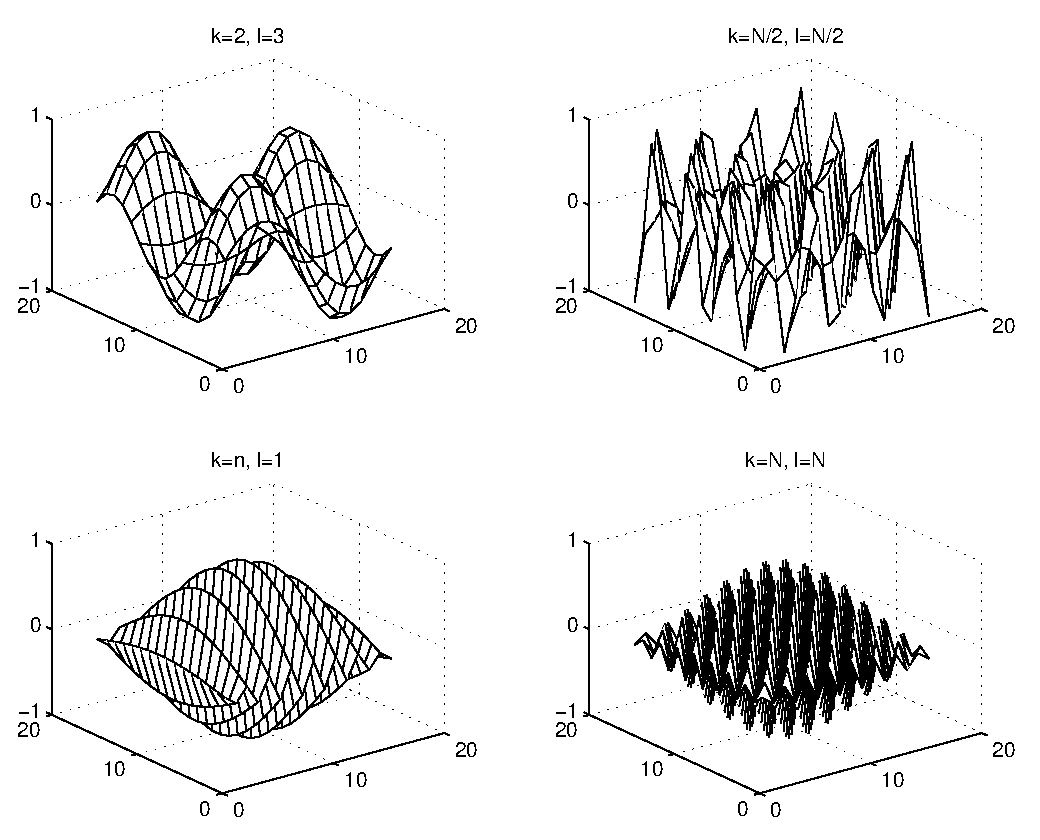
\includegraphics[scale=0.7]{eps/laplaceev}}
\caption{Ausgew\"ahlte Eigenvektoren f\"ur Modellproblem I}
\end{figure}

\subsection{Zweigitter-Verfahren}
Die Idee beim Zweigitter-Verfahren ist es jetzt, die L�sung f�r  $A_h$
durch eine L�sung f�r ein kleineres System
$A_{\hat h}$ mit gr\"o"serer Diskretisierungsweite $\hat{h}$ zu approximieren:
\begin{center}
\begin{picture}(125,85)
\drawline(0,80)(0,0)(120,0)(120,80)
\multiput(20,20)(40,0){3}{\circle{6}}
\multiput(40,20)(40,0){2}{\circle*{6}}
\multiput(20,40)(20,0){5}{\circle{6}}
\multiput(20,60)(40,0){3}{\circle{6}}
\multiput(40,60)(40,0){2}{\circle*{6}}
\end{picture}
\end{center}
Hier gilt $N=2\hat N+1$, also $\hat h=2\cdot h$.

\medskip

Wie Aufgabe~\ref{laplaceev_aufg} zeigt, gibt es Eigenvektoren, die einer starken Variation unterliegen, und Eigenvektoren, welche
eher "`glatt"' sind. Beim Verkleinern der Punktzahl jedoch k�nnen stark variierenden Eigenvektoren nur schlecht
approximiert werden. Darum unterteilen wir ($z^{(k,l)}$ seien Eigenvektoren f\"ur $A_h$)
\begin{align*}
X&:=\langle z^{(k,l)},\; k,\ l=1,\ \ldots,\ \hat N\rangle \quad (\text{"`glatte Vektoren"'} )\\
Y&:=\langle z^{(k,l)},\; k>\hat N \text{ oder } l>\hat N\rangle \quad (\text{"`oszillierende Vektoren"'} ).
\end{align*}

Es gilt dabei
\[
	\mathbb{R}^n=X\oplus Y \quad (n=N^2),
\]
weil die Eigenvektoren paarweise orthogonal zueinander sind.

\bigskip

Wir entwickeln nun ein Iterationsverfaren (�hnlich dem Schwarz-Verfahren) der folgenden Gestalt:

\fbox{\parbox{\linewidth-7pt}{
Gesucht ist der Fehler $e^k$ mit $x^*=x^k+e^k$. Statt dessen betrachten wir $r^k=b-A_h x^k$ (denn $A_he^k = A_h(x^*-x^k) = b - A_hx^k = r^k$).
\begin{enumerate}
\item Gl�tte $r^k$, d.h. bestimme $y^k$ so dass f\"ur $
s^k=b-A_hy^k$ gilt
\[
s^k \in X.
\]

\item Transportiere $s^k$ auf das grobe Gitter und bezeichne das Ergebnis mit $\hat s^k$. L�se
\[
A_{\hat h}\hat e^k=\hat s^k.
\]
Transportiere $\hat e^k$ auf das feine Gitter in $e^k$ und setze
\[
x^{k+1}=y^k+e^k.
\]
\end{enumerate}
}}

Anschaulichen entfernen wir aus $r^k$ die stark oszillierenden Komponenten.
\end{bsp}

\begin{defn}[Transportoperationen]
\begin{enumerate}
\item Die {\em Prolongation} $P$ (Abbildung von $\Omega_{\hat h}$ nach $\Omega_h$) ist als gewichtete Mittelung der acht Nachbar-Werte
definiert.
\begin{center}
\begin{picture}(190,160)
\multiput(20,0)(40,0){5}{\circle{6}}
\multiput(20,40)(80,0){3}{\circle{6}}
\multiput(60,40)(80,0){2}{\circle*{6}}
\multiput(20,80)(40,0){5}{\circle{6}}
\multiput(20,120)(80,0){3}{\circle{6}}
\multiput(60,120)(80,0){2}{\circle*{6}}
\multiput(20,160)(40,0){5}{\circle{6}}
\put(60,40){\vector(1,1){38}}
\put(140,40){\vector(-1,1){38}}
\put(60,120){\vector(1,-1){38}}
\put(140,120){\vector(-1,-1){38}}

\put(60,40){\vector(1,0){36}}
\put(140,40){\vector(-1,0){36}}

\put(75,110){$\frac{1}{4}$}
\put(120,110){$\frac{1}{4}$}

\put(59,50){$\frac{1}{4}$}
\put(135,50){$\frac{1}{4}$}

\put(80,25){$\frac{1}{2}$}
\put(115,25){$\frac{1}{2}$}
\end{picture}
\end{center}
bzw. in Sternform
\[
P=\left]\begin{array}{ccc}
\frac{1}{4}&\frac{1}{2}&\frac{1}{4}\\
\frac{1}{2}&1&\frac{1}{2}\\
\frac{1}{4}&\frac{1}{2}&\frac{1}{4}
\end{array}\right[ \quad  .
\]
$P$ ist eine $(\hat n\times n)$-Matrix, in welcher der Stern �ber die Zeilen verteilt ist. Dies ist eine bilineare Interpolation.

\item Die {\em Restriktion} $R$ als Abbildung von $\Omega_{ h}$
nach $\Omega_{\hat h}$ ist gegeben durch
\begin{center}
\begin{picture}(110,110)
\multiput(20,20)(40,0){3}{\circle{6}}
\multiput(20,60)(80,0){2}{\circle{6}}
\multiput(60,60)(80,0){1}{\circle*{6}}
\multiput(20,100)(40,0){3}{\circle{6}}

\put(20,20){\vector(1,1){38}}
\put(100,20){\vector(-1,1){38}}
\put(20,100){\vector(1,-1){38}}
\put(100,100){\vector(-1,-1){38}}

\put(20,60){\vector(1,0){36}}
\put(100,60){\vector(-1,0){36}}
\put(60,20){\vector(0,1){36}}
\put(60,100){\vector(0,-1){36}}

\put(8,97){$\frac{1}{16}$}
\put(8,57){$\frac{1}{8}$}
\put(8,17){$\frac{1}{16}$}

\put(105,97){$\frac{1}{16}$}
\put(105,57){$\frac{1}{8}$}
\put(105,17){$\frac{1}{16}$}

\put(65,97){$\frac{1}{8}$}
\put(65,17){$\frac{1}{8}$}
\put(70,60){$\frac{1}{4}$}
\end{picture}
\end{center}
bzw. in Sternform
\[
R=\frac{1}{4} \cdot \left]\begin{array}{ccc}
\frac{1}{4}&\frac{1}{2}&\frac{1}{4}\\
\frac{1}{2}&1&\frac{1}{2}\\
\frac{1}{4}&\frac{1}{2}&\frac{1}{4}
\end{array}\right[ \quad  .
\]
\end{enumerate}
Es gilt also $R=\frac{1}{4}\cdot P^T, \quad R\in\mathbb{R}^{\hat n \times n}, \quad P\in\mathbb{R}^{n \times \hat n},\ n=N^2,\ \hat n =\hat N^2$.
\end{defn}

\begin{bem}Die triviale Restriktion 
\[
R=
\left]\begin{array}{ccc}
0&0&0\\
0&1&0\\
0&0&0
\end{array}\right[
\]
ist f�r die Theorie und die Praxis weniger geeignet.
\end{bem}

Um die Frage des "`Gl�ttens"' zu behandeln, betrachten wir  das ged�mpfte Gesamschritt-Verfahren
\[
	y^{\nu+1}=y^\nu+\omega\cdot  D^{-1} r^\nu, \quad \omega \text{ D�mpfungsfaktor,}
\]
wobei $A=D-B,\ D=\diag(A),\ \nu=0,\ 1,\ \ldots$ Es gilt
\[
	r^{\nu+1}=((1-\omega ) I+\omega D^{-1}B)r^\nu.
\]
Setze $J_\omega:=(1-\omega ) I+\omega D^{-1}B$. Wir wissen: $J_\omega$ besitzt die Eigenvektoren $z^{(k,l)}$ mit den Eigenwerten
\[
	\mu_{k,l}^{(\omega)}=\frac{\omega}{2}\left(\cos(\pi\cdot k\cdot h)+\cos(\pi\cdot l\cdot h) \right)+(1-\omega).
\]
F�r die oszillierenden Eigenvektoren (d.h. $k>\frac{N-1}{2}$ oder $l>\frac{N-1}{2}$) gilt:
\[
	-2<\cos(\pi\cdot k\cdot h)+\cos(\pi\cdot l\cdot h)<1,
\]
also gilt f\"ur diese $k$ und $l$
\[
	|\mu_{k,l}^{(\omega)}|\le \max\left\{ \left|1-\frac{\omega}{2}\right|,\ |1-2\omega|\right \}, \quad  \omega>0.
\]
Die rechte Seite wird minimal f�r $\omega=\frac{4}{5}$ mit Wert $\frac{3}{5}$. 

\medskip

Wir halten fest:
\begin{lem} F�r $\omega\in\left[0,\frac{4}{5} \right]$ gilt
\begin{align*}
\frac{\omega}{2}\left(\cos(\pi\cdot k\cdot h)+\cos(\pi\cdot l\cdot h) \right)+(1-\omega)
	&\le  \max\left\{ \left|1-\frac{\omega}{2}\right|,\ |1-2\omega|\right \}\\
	&=1-\frac{\omega}{2}.
\end{align*}
\end{lem}

Damit haben wir alle Zutaten f�r ein Zweigitter-Verfahren beisammen.

\begin{defn} $y=S_{\nu,\omega}(x)$ bedeute $\nu$ Schritte der Gl�tterungsiteration angewendet auf $x$.
\end{defn}

\begin{alg}[Zweigitter-Verfahren]
~               % um "Algorithmus" aus dem Kasten rauszubekommen
\vspace*{-2\baselineskip}       % um den Leeraum zu entfernen
\begin{algorithm}
\begin{algorithmic}
\STATE w�hle $x^0$, setze $r^0=b-A_h x^0,\ \omega=\frac{4}{5}$
\FOR{$k=0,\ 1,\ \ldots$}
\STATE $y^k = S_{\nu,\omega}(x^k)$
\STATE $s^k = b-A_hy^k$ \COMMENT{$s^k$ ist glatt}
\STATE $\hat s^k = Rs^k$
\STATE l�se $A_{\hat h}\hat e^k = \hat s^k$
\STATE $e^k = P\hat e^k$
\STATE $x^{k+1} = x^k+e^k$
\ENDFOR
\end{algorithmic}
\end{algorithm}
\end{alg}

\begin{aufg}
Implementiere das Zweigitter-Verfahren f�r das Modellproblem I. Verwende direkten L�ser f�r $A_{\hat h}$ und messe
die Iterationszahlen abh�ngig von $\nu$ und $h$.
\end{aufg}

\begin{figure}[h!]
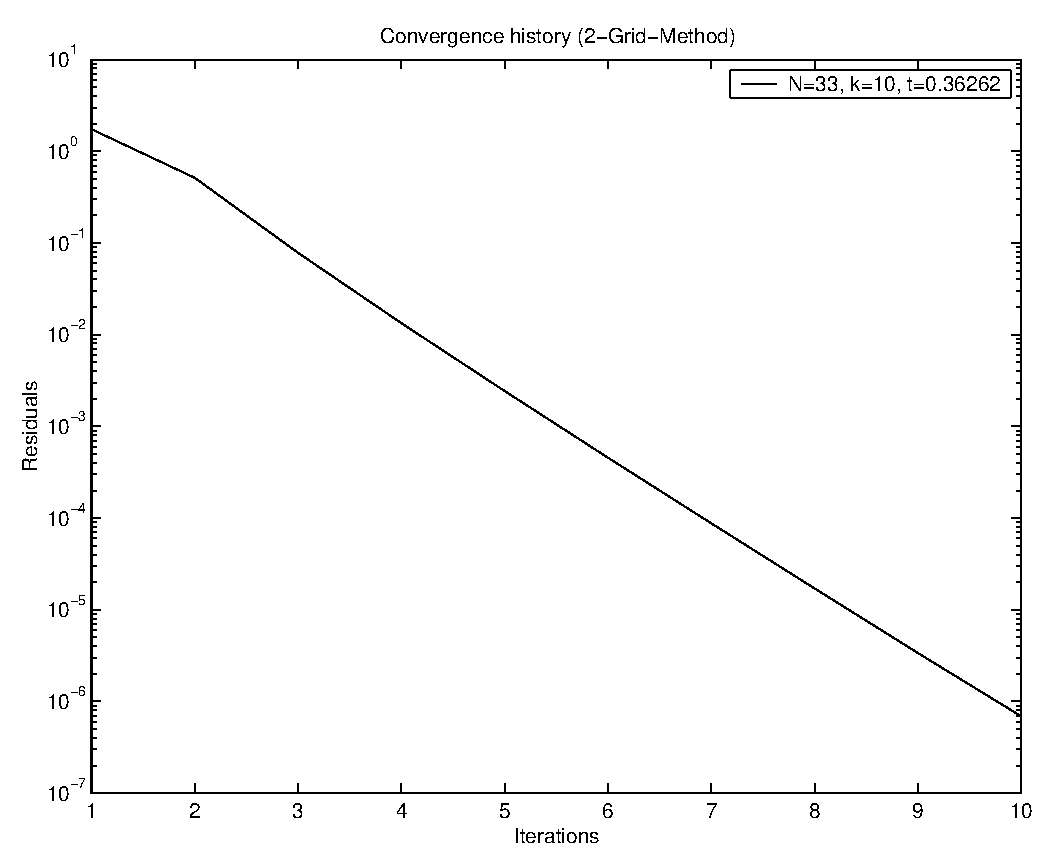
\includegraphics[scale=0.37]{eps/mp1mg2N33.eps}\hfill
\includegraphics[scale=0.37]{eps/mp1mg2N65.eps}
\caption{Zweigitterverfahrten f\"ur Modellproblem 1, $N=33$ (links), $N=65$ (rechts)}
\end{figure}

\subsection{Mehrgitter-Verfahren}
Die L�sung von $A_{\hat h}\hat e^k=\hat s^k$ kann auch rekursiv erfolgen. Man hat dann eine Hierachie: \\
$A_{0}$: zu l�sendes System \\
$A_{1}$: kleineres System mit zugeh�rigen Operatoren $P_1$ und $R_1$
\begin{center}
 $\vdots$
\end{center}
$A_{l_{max}}$: kleinstes System mit Operatoren $P_{l_{max}}$ und $R_{l_{max}}$ \\

Dem entspricht eine Hierachie von Gl�ttern: \\
$S^0_{\nu, \omega}$\\
\hspace*{0.25cm}$\vdots$ \\
$S^{l_{max}}_{\nu, \omega}$ \\

Das Mehrgitter-Verfahren ist dann gegeben durch:
\begin{alg}[Mehrgitter-Verfahren]
~               % um "Algorithmus" aus dem Kasten rauszubekommen
\vspace*{-2\baselineskip}       % um den Leeraum zu entfernen
\begin{algorithm}
\begin{algorithmic}
\STATE w�hle $x^0$, w"ahle $\gamma \in \{1,2,\ldots\}$ 
\FOR{$k=0,\ 1,\ \ldots$}
\item  $x^{k+1} = mgs(x^k, b, \gamma , 0 )$ \\
\ENDFOR
\end{algorithmic}
\end{algorithm}
\end{alg}

\begin{bem}
Dabei ist $mgs$ der noch zu definierende Mehrgitter-Schritt.
\end{bem}

\begin{alg}[Mehrgitter-Schritt $y = mgs(x, r,\gamma,l)$]
~               % um "Algorithmus" aus dem Kasten rauszubekommen
\vspace*{-2\baselineskip}       % um den Leeraum zu entfernen
\begin{algorithm}
\begin{algorithmic}[1]
%\IF{ $l=l_{max}$}
%\STATE l�se $A_{l_{max}} y = r$
%\ELSE
\STATE $x = S^l_{\nu, \omega}(x) $ \COMMENT{Vorgl\"attung}
\STATE $s = r - A_l x$
\STATE $\hat{s} = R_l s $
\STATE $\hat{x} = 0 $
\IF[auf gr"obstem Gitter, Rekursion beenden]{ $l+1=l_{max}$}
\STATE l�se $A_{l_{max}} \hat{x} = \hat{s}$
\ELSE
   \FOR{$\mu = 1, \ldots , \gamma $}
      \STATE $\hat x = mgs(\hat{x}, \hat{s}, \gamma, l+1)$
    \ENDFOR
\ENDIF
\STATE $e = P \hat{x}$
\STATE $y = x + e $
\end{algorithmic}
\end{algorithm}
\end{alg}

\begin{bem}
Je gr\"o"ser $\gamma$ gew\"ahlt wird, desto genauer wird die in der Schleife �ber $\mu$ berechnete
Approximation $\hat x$ f\"ur $A_{l+1}^{-1} \hat s$. �bliche Werte sind $\gamma = 1$ oder $\gamma = 2$.
Nach Zeile 11 kann noch ein "`Nachgl\"attungsschritt"' $e = S^l_{\mu, \omega}(e)$ eingeschaltet werden.
\end{bem}

\begin{figure}
\centerline{\includegraphics[scale=0.5]{eps/zyklen}}
\caption{V-Zyklus ($\gamma = 1$) und W-Zyklus ($\gamma = 2$) im Mehrgitterverfahren}
\end{figure}


\appendix

\section{L�sungs-Versuche}

\begin{aufg}
Finde ausgehend von Satz \nref{Minmaxkreis_sa} die L"osung von
\[
\underset{p_m\in \overline{\Pi}_m,}{\min}\ \underset{\lambda\in D(\gamma,\rho)}{\max}|p_m(\lambda)|.
\]
\end{aufg}
\textbf{Antwort:}
$p_m(z)=\frac{(z+\gamma)^m}{\gamma^m}$, wie man leicht mittels linearer Transformation $z\mapsto z-\gamma$
aus Satz \ref{Minmaxkreis_sa} einsieht.


\begin{aufg}
Bestimme jeweils die (im Sinne von Satz \nref{cmschranke_sa}) asymptotisch optimale L�sung der MinMax-Aufgabe
\[
\underset{p_m \in \overline{\Pi}_m }{\min} \quad \underset{\lambda \in E}{\max} |p(\lambda)|
\]
und den zugeh�rigen Wert des Minimums f�r die F�lle:
\begin{enumerate}
\item $E = a + bE_{\rho}$, wobei $a,b > 0$ und $ a - b\cdot \frac{1}{2}(\rho+1/\rho)  > 0 $
\begin{center}
\begin{picture}(200,100)
\put(150,50){\ellipse{80}{40}}
\put(150,30){\line(0,1){40}}
\put(0,50){\vector(1,0){200}}
\put(100,0){\vector(0,1){100}}
\end{picture}
\end{center}

\item $E = a+be^{i\frac{\pi}{2}}E_{\rho}$, wobei $a,b > 0$ und $ a - b \cdot \frac{1}{2}(\rho-1/\rho) > 0 $
\begin{center}
\begin{picture}(200,100)
\put(150,50){\ellipse{40}{80}}
\put(150,10){\line(0,1){80}}
\put(0,50){\vector(1,0){200}}
\put(100,0){\vector(0,1){100}}
\end{picture}
\end{center}

\item $E_\rho$ ist Geradenst�ck parallel zur reellen Achse von $-a$ bis $+a$ mit Achsenabschnitt b auf der imagin�ren Achse
\begin{center}
\begin{picture}(200,100)
\put(70,70){\line(1,0){60}}
\put(61,58){$-a$}
\put(121,58){$+a$}

\put(0,50){\vector(1,0){200}}
\put(100,0){\vector(0,1){100}}
\end{picture}
\end{center}
Sind in diesem Fall die Polynom auch optimal f"ur endliches $m$? 
\end{enumerate}
\end{aufg}
\textbf{Antwort:}
\begin{Blist}{1. und 2.}
\item[1. und 2.] wurden mit den Tschebyscheff-Polynomen behandelt.
\item[3.]
\end{Blist}

\begin{aufg}
Sei $A \neq A^H$, aber mit einer der folgenden speziellen Eigenschaften:
\begin{enumerate}
\item $A^H = \overline{A} \in \cnn$ (z.B. bei der Diskretisierung der Maxwell-Gleichungen in der Elektrodynamik)
\item $A^HJ = J^HA,\ J \in \cnn,\ J=J^H$ (man nennt $A$ dann auch {\em 
$J$-hermitesch})
\item $A^TJ = J^TA,\ J \in \cnn$ (man nennt $A$ dann auch {\em $J$-symmetrisch})
\end{enumerate}
Zeige jeweils: F�r geeignete Wahl von $\tilde{r}^0$ (bzw. $w^0$) kann man den unsymmetrischen Lanczos-Prozess mit nur einer MVM mit $A$
(und eventuell einer zus�tzlichen mit $J$) durchf�hren 
(dies �bertr�gt sich dann auch auf BiCG).
\end{aufg}
\begin{proof}
\begin{enumerate}
\item 
\[
AV^m = V^{m+1} T_{m+1,m} \quad \text{und} \quad A^H W^m = W^{m+1} \overline{T}_{m+1,m}
\]
$\Longrightarrow A \overline{W}^m = \overline{W}^{m+1} T_{m+1,m}$. W�hle also $w^0 = \overline{v}^0$, dann gilt: $w^m = \overline{v}^m \forall m$
\item
\[
AV^m = V^{m+1} T_{m+1,m} \quad \text{und} \quad A^H W^m = W^{m+1} \overline{T}_{m+1,m}
\]
Ansatz: $w^i = Jv^i$, dann gilt: \[A^H W_m = A^H J V_m = J A V_m = \underbrace{J V_{m+1}}_{=W_{m+1}}T_{m+1,m}.\] 
Es mu� also gelten das $T_{m+1,m} \in \mathbb{R}^{(m+1) \times m }$
\[
\alpha_m = \langle A v^m, w^m \rangle = \langle A v^m, J v^m \rangle = \langle J^H A v^m, v^m \rangle \in \mathbb{R}
\]
denn: $(J^H A)^H = A^H J=JA=J^HA$
\[
\delta_m = \langle \overline{v}^m, \overline{w}^m \rangle = \langle \overline{v}^m, J \overline{v}^m \rangle \in \mathbb{R}
\]
da $J=J^H$
\item analog zu 2 mit dem Ansatz: $w^i = \overline{J v^i}$
\end{enumerate}
\end{proof}

%\include{aufgabe7.8}
\end{document}
